\documentclass[11pt, twoside]{article}

\newif\ifincludeall\includealltrue


%%\usepackage{listings}
%%\usepackage{chngcntr}


%\addtotoclist[float]{lol}
%\renewcommand*\listoflistings{\listoftoc[{\listoflistingscaption}]{lol}}

% Erlaube einfaches copy & paste aus der generierten pdf
\usepackage[T1]{fontenc}
% Erlaube überall underscore zu benutzen ohne \_ schreiben zu müssen
% https://tex.stackexchange.com/questions/20890/define-an-escape-underscore-environment 
\catcode`\_=12
\usepackage[utf8]{inputenc}

% Deutsche Bezeichnungen wie etwa "Inhaltsverzeichnis", statt "Contents"
% ngerman ist neue Rechtschreibung: https://tex.stackexchange.com/questions/67549/whats-the-difference-between-ngerman-and-german-in-babel
\usepackage[ngerman]{babel}

\babelhyphenation[ngerman]{Me-tho-de}



\usepackage{scrextend}
\addto\captionsenglish{\renewcommand{\bibname}{References}}

%\renewcaptionname{ngerman}{\contentsname}{Inhalt}           %Table of contents
%\renewcaptionname{ngerman}{\listfigurename}{Abbildungen}    %Figures
%\renewcaptionname{ngerman}{\listtablename}{Tabellen}        %Tables
%\renewcaptionname{ngerman}{\figurename}{Abb.}               %Figure
%\renewcaptionname{ngerman}{\tablename}{Tab.}                %Table
%\renewcaptionname{ngerman}{\bibname}{Literatur}             %Bibliography
  \newcaptionname{ngerman}{\listlistingname}{Listingverzeichnis} 
  %\renewcaptionname{ngerman}{\listingname}{Quelltext}      %Listing

% Deutsche Absätze
\parindent 0pt

\renewcommand{\baselinestretch}{1.25}


% Dieses Package ermöglich einfügen von Bildern mittels \includegraphics
\usepackage{graphicx}

% Zwinge Latex zum einfügen von bildern dort wo man sie im tex 
% Dokument hinterlegt mittels \begin{figure}[H]   
\usepackage{float}

% Ändere Highlight Color
\usepackage{color}
\definecolor{insertedCode}{RGB}{190, 230, 190}
\definecolor{inlineCodeColor}{RGB}{244, 246, 248}
\definecolor{highPrioColor}{RGB}{255, 0, 0}
\definecolor{mediumPrioColor}{RGB}{0, 255, 255}

% Syntax Highlighting 
% newfloat macht, dass KOMA zusammen mit minted funktioniert und den Listings die Kapitelnummer voranstellt und sie gruppiert, so, wie auch mit den Abbildungen 
% newfloat macht auch, dass durch die Verwendung von KOMA nun Befehle wie  \renewcommand{\listoflistingscaption}{Listingverzeichnis} nicht mehr funktionieren
% umbennenen des List of Listings funktioniert dann anders:
% nämlich so: \newcaptionname{ngerman}{\listlistingname}{Listingverzeichnis} (https://tex.stackexchange.com/questions/82993/how-to-change-the-name-of-document-elements-like-figure-contents-bibliogr)
% Achtung wegen minted nicht lstlistlistingname sondern listlistingname
\usepackage[newfloat]{minted}
% Lösche rote Rahmen in minted Quelltext und nutze das Visual Studio Theme
\usemintedstyle{vs}
\ifIncludeFigures
  \setminted{autogobble=true, fontsize=\footnotesize, baselinestretch=1.0, mathescape, linenos, numbersep=8pt, breaklines, highlightcolor=insertedCode, breakafter=_@|.}
\fi
%\renewcommand{\listingscaption}{Code Snippet}
% Veringere Abstand zum Untertitel
%\AtEndEnvironment{listing}{\vspace{-14pt}} % <-
% Bei Syntaxfehler keine roten vierecke darum zeichnen
% https://tex.stackexchange.com/questions/343494/minted-red-box-around-greek-characters 

% rounded corners for minted listings
\usepackage[]{mdframed}
\BeforeBeginEnvironment{mintinline}{\begin{mdframed}}
    \AfterEndEnvironment{mintinline}{\end{mdframed}}

\usepackage{etoolbox}

% Kann das Weg? Habe ich im Anhang anders gelöst denke ich
\makeatletter
\AtBeginEnvironment{minted}{\dontdofcolorbox}
\def\dontdofcolorbox{\renewcommand\fcolorbox[4][]{##4}}
\makeatother



\usepackage[autostyle,german=quotes]{csquotes}

% Für Hintergrundbilder mittels \AddToShipoutPicture
\usepackage{eso-pic}

% Bilder transparent machen
\usepackage{transparent}

% Fallunterscheidungen wie etwa gerade und ungerade Seiten
\usepackage{ifthen}

% Einfügen von Tabellen
\usepackage{tabularx}

% Literaturverzeichnisse verwenden
% backref=true -- referenziert von Literaturverzeichnis zurück auf die Seite wo zitiert wurde
%\usepackage[style=authortitle, natbib, backend=biber, backref=true]{biblatex}
\usepackage[%
  style=authortitle, % sorgt dafür dass in der Fußnote der Autor und dann der Titel gelistet wird, welches hiervon aber?
  natbib, % sorgt dafür dass in der Fußnote der Autor und dann der Titel gelistet wird, welches hiervon aber?
  backref=true % sorgt dafür dass in der Fußnote der Autor und dann der Titel gelistet wird, welches hiervon aber?
  backend=bibtex8, % KOMA benutzt bibtex8 statt biber
]{biblatex}
% Nummer der Zitation nicht hochgestellt, sondern sondern mit
% normaler Textgröße und einem Punkt nach der Nummer
% Beispiel: 1. Teller,”Visibility computations in densely occluded polyhedral environments.“, S. 19
\makeatletter% 
\long\def\@makefntext#1{% 
  \parindent 1em\noindent \hb@xt@ 1.8em{\hss  \hbox {{\normalfont \@thefnmark }}. }#1}%
\makeatother

% Texte für die zurückreferenzierung definieren
\DefineBibliographyStrings{german}{%
  backrefpage = {Zitiert auf der Seite},% originally "cited on page"
  backrefpages = {Zitiert auf den Seiten},% originally "cited on pages"
}



% Referezieren von Kapiteln mit ihrem Titel
\usepackage{nameref}

% Einfügen von PDFs
\usepackage{pdfpages}

% Seitenränder
\ifInfinitePaperLength
\usepackage[paperwidth=500cm,paperheight=21cm,margin=1in]{geometry}
\else
\usepackage{geometry}
\geometry{a4paper, top=20mm, inner=40mm, outer=20mm, bottom=20mm, headsep=12mm, footskip=12mm}
\fi




% Absatzformat
%\parskip2ex		% Absatzabsstand	
%\parindent0ex		% Absatzeinzug

% Package zum hinzufügen eines Glossars
\usepackage{glossaries}
\setacronymstyle{long-short}
\newacronym{eler}{ELER}{Europäischer Landwirtschaftsfond für die Entwicklung des ländlichen Raum}


% Abbildungsunterschrift anpassen
% https://tex.stackexchange.com/questions/86120/font-size-of-figure-caption-header/86121
\usepackage[font=footnotesize,labelfont=bf]{caption}
% Abstand anpassen
% https://tex.stackexchange.com/questions/45990/how-can-i-modify-vertical-space-between-figure-and-caption
\setlength{\abovecaptionskip}{10pt plus 3pt minus 2pt}

% Nutze unterschiedliche fußnoten (1,2,3 und a,b,c)
\usepackage[para]{manyfoot}
% \footnoteL{https://google.com}
\DeclareNewFootnote{L}[Roman]
% \footnoteI{https://google.com}
\DeclareNewFootnote{I}[alph]

% fußnoten nacheinander mit Kommas
% \footnote{Einz}\footnote{Zwei}
\usepackage[multiple]{footmisc}



% https://tex.stackexchange.com/questions/50654/how-to-allow-line-breaks-after-forward-slashes-in-context?rq=1
% enables a break point after /, +, (, ) and -
% use hyphens option to break url
\usepackage{url}
% \def\UrlBreaks{%
%   \do\/%
%   %\do\a\do\b\do\c\do\d\do\e\do\f\do\g\do\h\do\i\do\j\do\k\do\l%
%   %   \do\m\do\n\do\o\do\p\do\q\do\r\do\s\do\t\do\u\do\v\do\w\do\x\do\y\do\z%
%   %\do\A\do\B\do\C\do\D\do\E\do\F\do\G\do\H\do\I\do\J\do\K\do\L%
%   %   \do\M\do\N\do\O\do\P\do\Q\do\R\do\S\do\T\do\U\do\V\do\W\do\X\do\Y\do\Z%
%  \do\*\do\-\do\~\do\'\do\"\do\-\do\\%
%  \do\_
%  \do\l
%  \do\n
%  \do0\do1\do2\do3\do4\do5\do6\do7\do8\do9\do=\do/\do.\do:%
% }

\usepackage{xurl}

% Links mit Sprungmarken
% hyperref muss nach \usepackage[hyphens]{url} kommen, sonst gibt es einen Option clash, denn hyperref läd url ohne hyphens option
% https://tex.stackexchange.com/questions/50654/how-to-allow-line-breaks-after-forward-slashes-in-context?rq=1
\usepackage{hyperref}
\hypersetup{
  colorlinks=true,
  linkcolor=black, % Setz die Farbe von Links im 
  % Inhaltsverzeichnis zurück auf schwarz
  citecolor=black, % Farbe von Literaturlinks = schwarz
  urlcolor=blue    % Farbe von URLs = blau     
}

% Auf gleiche footnote erneut verweisen mit cleveref
% Achtung: Wenn cleveref nicht zum ende geladen wird gibt es evtl. die Fehlermeldung: Package cleveref Error: cleveref must be loaded after amsmath!.
\usepackage{cleveref}
% Auf erneut verweisen
\crefformat{footnote}{#2\footnotemark[#1]#3}


% Installation manuell: 
% Download: https://perso.ensta-paris.fr/~kielbasi/tikzuml/index.php?lang=en&id=download
% Kopieren nach texlive\texlive\2021\texmf-dist\tex\latex
% texhash ausführen
% uml diagramme mit tikz
\ifIncludeFigures
\usepackage{tikz-uml}
\fi

% Blindtext einfügen
\usepackage{blindtext}

% hintergrund für listings (auch inline)

\usepackage{tcolorbox}

\xdefinecolor{inlineCodetXColor}{RGB}{244,246,248}

\newtcbox{\inlineCodetcbox}[1][inlineCodetXColor]{on line,
  arc=1pt,colback=inlineCodetXColor,colframe=inlineCodetXColor,
  before upper={\rule[-3pt]{0pt}{10pt}},boxrule=0pt,
  boxsep=0pt,left=2pt,right=2pt,top=2pt,bottom=0pt}

\newtcolorbox{codeFrame}{colback=inlineCodetXColor,
  colframe=inlineCodetXColor,on line,arc=4pt,boxrule=0pt,boxsep=0pt,left=4pt,right=4pt,top=4pt,bottom=4pt}

\BeforeBeginEnvironment{minted}{\begin{codeFrame}}
    \AfterEndEnvironment{minted}{\end{codeFrame}}

\newcommand{\alexlistingcaption}[3]{\caption[#2]{#2\ifIncludeFigures, Quelle: Eigenes Listing, Datei: \url{#3}\fi}}


% Code Snippet -> Listing
%\renewcommand{\listingscaption}{Listing}
% Eigener Befehl für Listings
\newenvironment{alexlisting}[4]
{%
  \begin{listing}[ht]%
    \ifIncludeFigures
    \begin{codeFrame}
        \inputminted[#4]{dart}{#3}%
    \end{codeFrame}
    \fi
    %\vspace{-18pt}
    \alexlistingcaption{#1}{#2}{#3}%
    }%
    {%
  \end{listing}%
}


\newenvironment{alexyamllisting}[4]
{%
  \begin{listing}[ht]%
    \ifIncludeFigures

    \begin{codeFrame}
        \inputminted[#4]{yaml}{#3}%
    \end{codeFrame}
    \fi

    %\vspace{-18pt}
    \alexlistingcaption{#1}{#2}{#3}%

    }%
    {%
  \end{listing}%
}

\newcommand{\fremdeslistingcaption}[4]{\caption[#1 #2]{#2, Quelle: #4, Datei: \url{#3}}}
% Eigener Befehl für fremde Listings
\newenvironment{fremdeslisting}[6]
{%
    \begin{listing}[ht]%
      \ifIncludeFigures
      \begin{codeFrame}

      \inputminted[#4]{#6}{#3}%

    \end{codeFrame}
    \fi
      %\vspace{-18pt}

      \ifIncludeFigures
      \fremdeslistingcaption{#1}{#2}{#3}{#5}%
      \else
      \caption[#1]{#2}
      \fi
            }%
      {%
    \end{listing}%
}

% Eigener Befehl für Bilder
\newenvironment{alexfigure}[4]
{%
    \begin{figure}[ht]
      \centering
      %\ifIncludeFigures
      \includegraphics[width=1.0\textwidth]{#1}
      %\fi

      \ifIncludeFigures
      \caption[#2]{#3, Quelle: Eigene Abbildung}
      \else
      \caption[#2]{#3}
      \fi

      }%
      {%
    \end{figure}%
}

% Eigener Befehl für Bilder
\newenvironment{alexfigurewithnotebook}[5]
{%
    \begin{figure}[ht]
      \centering
      \ifIncludeFigures
      \includegraphics[width=1.0\textwidth]{#1}
      \fi
      \caption[#2]{#3, Quelle: Eigene Abbildung, Notebook:\url{#4}, Daten-Quelle:#5}
      }%
      {%
    \end{figure}
}


% Eigener Befehl für Abbbildungsreferenz
\newcommand{\Abb}[1]{%
\ifForDuden%
%
\else%
(Abb. #1)%
\fi%
}

% Eigener Befehl für Abbbildungsreferenz mit Seite
\newcommand{\AbbS}[1]{%
\ifForDuden%
%
\else%
(Abb. \ref{#1}, S. \pageref{#1})%
\fi%
}

% Eigener Befehl für Listingreferenz
\newcommand{\Lst}[1]{%
\ifForDuden%
%
\else%
(Listing #1)%
\fi%
}

% Eigener Befehl für Zeilenreferenz
\newcommand{\Z}[1]{%
\ifIncludeLineNumbers%
(Z. #1)%
\else%
\fi%
}
% Eigener Befehl für Listingreferenz mit Zeilenreferenz
\newcommand{\LstZ}[2]{%
\ifForDuden%
%
\else%
(Listing #1, Z. #2)%
\fi%
}

% Eigener Befehl für Listingreferenz mit Zeilenreferenz
\newcommand{\LstSZ}[2]{%
\ifForDuden%
%
\else%
(Listing \ref{#1}, S. \pageref{#1}, Z. #2)%
\fi%
}

\newcommand{\LstS}[1]{%
\ifForDuden%
%
\else%
(Listing \ref{#1}, S. \pageref{#1})%
\fi%
}

\ifForDuden%
\renewcommand{\footcite}{}%
\else%
\fi%



% Eigener Befehl für inline Code

\newcommand{\IC}[1]{%
\ifDingsInsteadOfInlineCode%
Dings%
\else%
\inlineCodetcbox{\mintinline[breaklines, breakafter=_/.]{dart}{#1}}%
\fi%
}
\newcommand{\C}[1]{\mintinline{dart}{#1}}

\newcommand{\HP}[1]{\mintinline[breaklines, breakafter=_/.,bgcolor=highPrioColor]{dart}{#1}}
\newcommand{\MP}[1]{\mintinline[breaklines, breakafter=_/.,bgcolor=mediumPrioColor]{dart}{#1}}




\newcommand{\DartSpec}[1]{%
\ifForDuden%
%
\else%
\footcite[Vgl.][S. #1]{DartProgrammingLanguageSpecification5thedition}%
\fi%
}
\newcommand{\JavaSpec}[1]{%
\ifForDuden%
%
\else%
\footcite[Vgl.][S. #1]{TheJavaLanguageSpecificationJavaSE16Edition}%
\fi%
}
% Abstand zwischen itemize Punkten verringern
% https://stackoverflow.com/questions/2180567/change-parskip-only-inside-enumerate-itemize-environment

% Package inputenc: Unicode char ³ (U+B3) (inputenc)	not set up for use with LaTeX.
% https://tex.stackexchange.com/questions/83440/inputenc-error-unicode-char-u8-not-set-up-for-use-with-latex
\DeclareUnicodeCharacter{00A0}{ }
% https://tex.stackexchange.com/questions/435302/unicode-character-error-inputenc-package
\DeclareUnicodeCharacter{00B3}{\textsuperscript{3}}

% enquote wird auch immer kursiv gesetzt
\let\oldenquote\enquote
% \renewcommand{\enquote}[1]{\textit{\oldenquote{#1}}} % <--  mit Anfügrungsstrichen
\renewcommand{\enquote}[1]{%
\ifDingsInsteadOfEnqoute%
Dings%
\else%
\textit{#1}%
\fi%
}



% Anleitung zum Styling vom Kapitel Titel
% https://tex.stackexchange.com/questions/50448/how-to-place-the-chapter-number-behind-the-chapter-title-in-koma-script


% roman numbering
\renewcommand{\thepart}{\Roman{part}}
% remove dot after number
\renewcommand{\partformat}{\partname~\thepart}
% font for "Part X"
\setkomafont{partnumber}{\normalsize\rmfamily}
% font for part title
\definecolor{flutterDarkBlue}{RGB}{7, 89, 157}
\setkomafont{part}{\huge\rmfamily\color{flutterDarkBlue}\textsc}

% Multiple Choice boxes https://tex.stackexchange.com/questions/81938/multiple-choice-with-answers-at-the-end-of-the-chapter
\usepackage{enumitem,amssymb}


% pdf kommentare
\usepackage[author={Alexander Johr}]{pdfcomment}

% Tabellen, mit span
\usepackage{multirow,tabularx}
% Eigene Spalte
\newcolumntype{Y}{>{\centering\arraybackslash}X}
\renewcommand{\arraystretch}{1.5}

\usepackage{tabu}
\usepackage{longtable}
\usepackage{makecell}
\usepackage{multirow}


\ifIncludeFigures

\else
  \renewcommand{\cleardoublepage}{}
  \renewcommand{\clearpage}{}
\fi

\usepackage[all]{nowidow}


\usepackage{dirtytalk}
 

\addbibresource{Literatur/Literatur.bib}

\begin{document}

\setcounter{page}{0}
% todo high: uncomment 
%\newpage\null\thispagestyle{empty}\newpage
% todo high: uncomment
\begin{titlepage}
    \begin{center}


        %\includegraphics[width=0.5\paperwidth]{img/logo/hs_harz_logo.png}

        \vspace{30mm}


        \vfill
        \vfill




        \vfill


        \LARGE{\textsc{Entwicklung einer Formularanwendung mit Kompatibilitätsvalidierung der Einfach- und Mehrfachauswahl-Eingabefelder}}


        \vfill
        \vfill
        \vfill
        \vfill

        % https://pascalhertleif.de/artikel/richtlinien-fur-fallstudien-in-der-software-entwicklung/

        \normalsize
        Vorgelegt von:

        \textbf{Alexander Johr}

        Meine Adresse

        \vspace{20mm}

        \begin{tabular}{r c}
            Erstprüfer:  & Prof. Jürgen Singer Ph.D. \\
            Zweitprüfer: & Prof. Daniel Ackermann    \\
            Datum:       & 02.11.2020                \\
        \end{tabular}

        \vspace{5mm}

    \end{center}

\end{titlepage} 
% todo high: uncomment \newpage\null\thispagestyle{empty}\newpage
% todo high: uncomment \ifincludeall

    
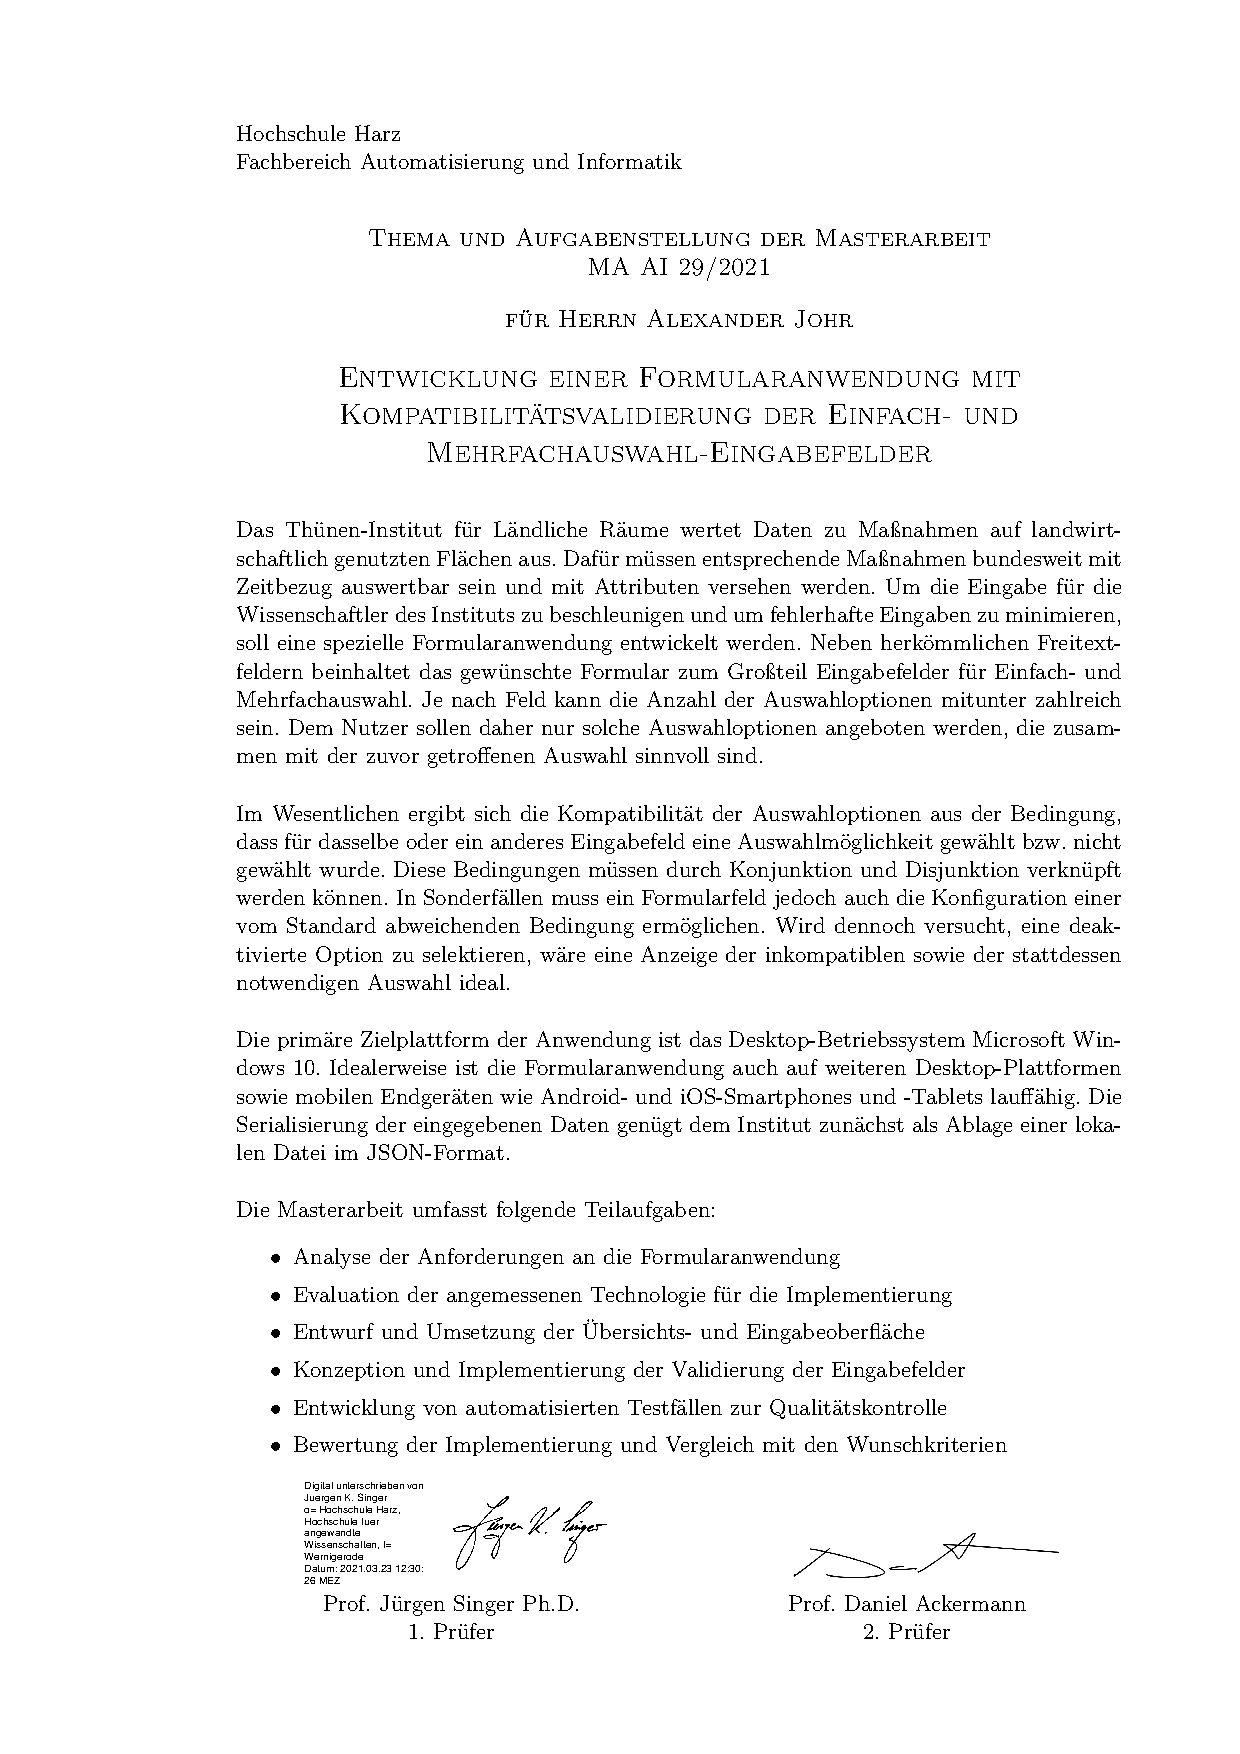
\includepdf[pages=-]{Inhalt/Expose/Masterarbeit-Expose-AJohr-27007.pdf}


    % 
\newpage
\thispagestyle{empty}

Hochschule Harz\newline
Fachbereich Automatisierung und Informatik
\vfill
\begin{center}

\large{\textsc{Thema und Aufgabenstellung der Masterarbeit}}

\large{\textsc{MA AI 29/2021}}

\vfill

\large{\textsc{für Herrn Alexander Johr}}

\vfill

%\vfill
\Large{\textsc{Entwicklung einer Formularanwendung mit Kompatibilitätsvalidierung der Einfach- und Mehrfachauswahl-Eingabefelder}}



\end{center}

\vfill

%gut darlegen könnendie methode spielt mehr die rolle


%andeuten nicht ins detail

%ich möchte mich testing


%kern des themas

%immer zurück kommen

%höhere eigen zum ergebis

%das liebesleben der tennisbällen unter einfluss des mondscheins

%größtmögliche unfall der passiert mal wahrscheinlichkeit 

%kompliziertheit komplexität

%werner von braun
%triebwerke geschrottet

%doku 
%arte 3 sat
%allgemein menschheit in den weltraum

%feindifferenziert


%Frage an Herr Ackermann / Singer: Vergleich mit Angular Dart, Angular allgemein, XAML WPF, evtl. etwas 

%Aber nicht alle

%Deshalb Fallstudie, richtig?

Das Thünen-Institut für Ländliche Räume wertet Daten zu Maßnahmen auf landwirtschaftlich genutzten Flächen aus. Dafür müssen entsprechende Maßnahmen
bundesweit mit Zeitbezug auswertbar sein und mit Attributen versehen werden.
Um die Eingabe für die Wissenschaftler des Instituts zu beschleunigen
 und um fehlerhafte Eingaben zu minimieren, soll eine 
 spezielle Formularanwendung entwickelt werden.
Neben herkömmlichen Freitextfeldern beinhaltet das gewünschte Formular zum Großteil Eingabefelder für Einfach- und Mehrfachauswahl.
Je nach Feld kann die Anzahl der Auswahloptionen mitunter zahlreich sein.
Dem Nutzer sollen daher nur solche Auswahloptionen angeboten werden,
die zusammen mit der zuvor getroffenen Auswahl sinnvoll sind.

\vspace{14pt}

Im Wesentlichen ergibt sich die Kompatibilität 
der Auswahloptionen aus der Bedingung, 
dass für dasselbe oder ein anderes Eingabefeld eine Auswahlmöglichkeit gewählt bzw.
nicht gewählt wurde. Diese Bedingungen müssen durch 
Konjunktion und Disjunktion verknüpft werden können.
In Sonderfällen muss ein Formularfeld jedoch auch 
die Konfiguration einer vom Standard abweichenden Bedingung
ermöglichen. 
Wird dennoch versucht,
eine deaktivierte Option zu selektieren, wäre eine Anzeige der
inkompatiblen sowie der stattdessen notwendigen Auswahl ideal.

\vspace{14pt}
Die primäre Zielplattform der Anwendung ist das Desktop-Betriebssystem
Microsoft Windows 10.
Idealerweise ist die Formularanwendung auch auf weiteren Desktop-Plattformen sowie
mobilen Endgeräten wie Android- und iOS-Smartphones und -Tablets
lauffähig. Die Serialisierung der eingegebenen Daten genügt dem Institut 
zunächst als Ablage einer lokalen Datei im JSON-Format. 
%Nach der Testphase des Eingabeformulars erfolgt der Import der Daten in das Relationale Datenbank-Management System ProstgreSQL. 

% Beim Versuch, eine inkompatible Auswahl zu selektieren,
% könnte die Visualisierung eines Mengendiagramms der erforderlichen und invaliden
% Auswahlfelder und die User Experience weiter verbessern.
% Als Ergebnis der Anforderungsanalyse wurde 
% ein UI-Framework ausgewählt,
% welches neben weiteren Auswahlkriterien 
% insbesondere ein hohes Maß an Flexibilität erlaubt: Flutter.





%Die freiheiten in der Oberflächenentwicklung 


%Ziel dieser Masterarbeit ist die Entwicklung der Formular-Anwendung 
%und dabei den Entwicklungsschitteprozess und die 

%Flutter bietet arbeitet mit funktionaler UI. Damit gibt Flutter die Wahl des Zustandsmanagements.


%Dies bietet einige Vorlteile. Koontrolle über die Performance.
%Vereinfachte Fehlersuche in der UI. Freiheiten in der Entwicklung der UI.
%Konfiguration von wiederverwendbaren Oberflächenkomponenten mithilfe des Strategy Entwurfsmusters.
%Doch es ergeben sich auch Nachteile: 
%Es gibt keine goto Methode für zustandsmanagement sondern eine Auswahl der 
%richtigen Methoe muss auf Grundlage der Anfforderungen gewählt werden.

%Zier der Arbeit ist es die Vorteile und Nachteile näher zubeleuchten.
%Dies soll mit der Entwicklung einer Anwendung in Flutter begleitet werden. Die Anwendung soll eine komplexes Eingabe-Formular für das Thünen institut in Braunschweig sein.



%Templates <-> Functional UI

%Exceptions <-> Hot Reload

%Stragety Pattern

%Reguläre ausdrücke

%Refactoring

%Programmgenerierung JSON AOT vs C\# Reflection


%Kontrolle

%Nachteile

%Provider BloC <-> Provider
%Eine  Data Binding

%Die zwei b Die beiden 

%Performance

%Die Produkte QlikView und Qlik Sense - Business Intelligence Software des Software\-unter\-nehmens Qlik - bieten ihren Anwendern mit einer Reihe an unterschiedlichen Diagramm\-typen einen Überblick über ihre Geschäftsdaten mittels Ad-hoc-Analysen. Nicht alle Wünsche der Anwender lassen sich über die Konfigurations\-möglich\-keiten dieser vorgefertigten Diagramme abdecken. Eine Alternative stellen die sogenannten Extension Objects und Document Extensions dar, die mit mithilfe von Webtechnologien wie JavaScript, HTML, CSS und XML entwickelt werden können. Die Entwicklung von Programmen mit JavaScript erweist sich jedoch gegenüber der Entwicklung mit anderen Programmiersprachen als sehr mühsam.


%Ziel dieser Bachelorarbeit ist es die Entwicklung dieser Extension Objects sowie Document Extensions mit der Programmiersprache Dart von Google umzusetzen, da sich diese für die Entwicklung skalierbarer und strukturierter Webanwendungen eignet. Die Arbeit bietet einen Leitfaden wie solche Extensions mit Dart entwickelt werden können und welche Vor- und Nachteile dies gegenüber der Entwicklung mit JavaScript bietet. 


%Die Bachelorarbeit beinhaltet folgende Teilaufgaben:
%\begin{itemize}
%	\itemsep0em
%	\item Analyse der Unterschiede von QlikView 11 und Qlik Sense bei der Entwicklung von Extension Objects sowie von Document Extensions
%	\item Analyse der Einschränkungen von Extensions Objects gegenüber der von QlikView 11 und Qlik Sense mitgelieferten Sheet Objects
%	\item Analyse der Auswirkungen der Extensions auf die Performance
%	\item Analyse der Vor- und Nachteile der Entwicklung von Extensions mit Dart im Vergleich zur Entwicklung von Extensions mit JavaScript
%	\item Entwicklung von zeitsparenden Methoden zur Entwicklung von Extensions
%	\item Bewertung der Ergebnisse
%\end{itemize}

\vspace{14pt}
Die Masterarbeit umfasst folgende Teilaufgaben:
\begin{itemize}
    \itemsep0em
\item Analyse der Anforderungen an die Formularanwendung
\item Evaluation der angemessenen Technologie für die Implementierung
\item Entwurf und Umsetzung der Übersichts- und Eingabeoberfläche
\item Konzeption und Implementierung der Validierung der Eingabefelder
\item Entwicklung von automatisierten Testfällen zur Qualitätskontrolle
\item Bewertung der Implementierung und Vergleich mit den Wunschkriterien
\end{itemize}


%Die Freiheiten der Oberflächenentwicklung in Flutter sollen genutzt werden, um 
%visuellen Komponenten zu erstellen, die durch Einsatz des Strategie-Entwurfsmusters
%im hohen Maße anpassbar sind.



%Da die Aktualisierung von Flutter-Views nicht automatisch erfolgt, muss ein angemessenes 
%Zustandsmanagement evaluiert und eingesetzt werden.
%Eine angemessene Technologie zur Serialisierung soll gewählt und 
%das Persistieren der eingegebenen Datensätze damit umgesetzt werden.
%Durch die Menge der Auswahlfelder ist bei Weiterentwicklung der APIs mit 
%hohem Migrationsaufwand der Codebasis zu rechnen. Der Einsatz von regulären Ausdrücken
%soll helfen, den Prozess zu automatisieren. Die Entwicklung automatisierter Testfälle
%soll weiterhin ermöglichen, Fehler bei der Weiterentwicklung zeitnah zu erkennen.



%Die Masterarbeit beinhaltet damit folgende Teilaufgaben:
%\begin{itemize}
%	\itemsep0em
%	\item Evaluation des Zustandsmanagements und Implementierung des View Models
%    \item Entwicklung von wiederverwendbarer Komponenten des Views und Anpassung dieser mit dem Strategie Entwurfsmuster
%    \item Auswahl der Technologie zur Serialisierung und Implementierung der Persistierung des Models
%	\item Migration der Codebasis auf aktualisierte APIs mittels Regulärer Ausdrücke
%	\item Entwicklung von Automatisierten Testfällen
%\end{itemize}

\vfill
\vfill
\vfill 
\vfill
\vfill

\begin{tabularx}{\textwidth}{@{} *2{>{\centering\arraybackslash}X}@{}}
Prof. Jürgen Singer Ph.D. & Prof. Daniel Ackermann \\
1. Prüfer                 & 2. Prüfer	 \\
\end{tabularx}	     



\fi   

% todo high: uncomment \newpage\null\thispagestyle{empty}\newpage 
% todo high: uncomment \tableofcontents
% todo high: uncomment \listoffigures 
% todo high: uncomment %List of Listings umbenennen
\renewcommand{\listoflistingscaption}{Listingsverzeichnis}

%Listingsverzeichnis
\addcontentsline{toc}{section}{Listingsverzeichnis}
\listoflistings

% todo high: Löschen!
% todo high: uncomment \section{Anforderungen}

Dieses Kapitel behandelt die Anforderungen

\begin{itemize}
    \item Performance: Hohe Anzahl Eingabefelder
    \item nested formulars
\end{itemize}


Wunsch
\begin{itemize}
	\item Alle Komponenten wiederverwendbar wie etwa Selection Caard nicht nur für Choices
	\item 
\end{itemize}

\begin{itemize}
	\item Strategy Entwurfsmuster für compute choice von viewModelType weil viewmodel nötig ist für nested formular
	\item 
\end{itemize}

% todo high: uncomment 
\part{Einleitung} 


\section{Problemstellung}

Das primäre Problem der Formular-Anwendung ist, dass sich die Auswahlfelder untereinander beeinflussen.
Wird eine Option in einem Auswahlfeld selektiert, so werden die möglichen Auswahlfelder von potenziell jedem anderen Auswahlfeld dadurch manipuliert.
Es muss eine Möglichkeit gefunden werden, die Abhängigkeiten in einer einfachen Art und Weise für jede Auswahloption zu hinterlegen und bei Bedarf abzurufen.


Das sekundäre Problem, welches sich vom primären Problem ableiten lässt, ist die  Laufzeit-Geschwindigkeit. 
Wenn die Auswahl in einem Auswahlfeld die Auswahlmöglichkeiten in potenziell allen anderen Auswahlfeldern manipuliert, so könnte dies zu einer hohen Last beim erneuten Zeichnen der Oberfläche zur Folge haben.
Wann immer der Nutzer eine Selektion tätigt, müsste das gesamte Formular neu gezeichnet werden, um sicherzustellen, dass invalide Auswahloptionen gekennzeichnet werden.
Bei einem  Formular mit wenigen Auswahlfeldern wäre das kein Problem.
Doch die nötigen Auswahlfelder für das Eintragen von Maßnahmen  des Europäischen Landwirtschaftsfonds für die Entwicklung des ländlichen Raums (ELER) sind zahlreich.
Ein  automatisierter Integrationstest, welcher im Formular Daten einer beispielhaften Maßnahme einträgt, zählt zum Zeitpunkt der Erstellung dieser Arbeit bereits 58 aufgerufene Auswahlfelder und 107 darin selektierte Auswahloptionen.
Das bedeutet, dass bei jedem dieser 107 Selektionen die 58 Auswahlfelder und all ihre Kinder neu gezeichnet werden müssten.
Es könnten also Wartezeiten nach jedem Auswählen einer Option entstehen.
Das Formular soll in Zukunft zudem noch erweitert und auch für die Eingabe ganz anderer Datensätze mit potenziell noch mehr Auswahlfeldern eingesetzt werden.
Es ist also erforderlich, dass ein Mechanismus gefunden wird,  der nur die Elemente neu zeichnet, die sich wirklich ändern.

\input{Inhalt/Einleitung/Abhängigkeiten-unter-den-Auswahlfeldern}


Für Form wurde Flutter gewählt

\section{Grundlagen}

Für die Formular Anwendung wurde die Programmiersprache Dart und das Oberflächen Framework Flutter gewählt. Kapitel Kapitel einfügen  erläutert die Entscheidungs-Grundlage dafür.

Nachfolgend soll auf  Grundlagen der beiden Technologien eingegangen werden.

\subsection{Flutter}

Flutter ist ein Framework zur Entwicklung von Oberflächen von Google.
Es unterstützt eine breite Anzahl an Ziel-Systemen.  Dazu gehören:

\begin{itemize}
  \item Desktop:\footcite[Vgl.][]{DesktopSupportForFlutter}
        \begin{itemize}
          \item Windows:
                \begin{itemize}
                  \item Win32,
                  \item Universal Windows Platform,
                \end{itemize}
          \item macOS,
          \item Linux,
        \end{itemize}
  \item Mobile Endgeräte\footcite[Vgl.][]{FlutterBeautifulNativeAppsInRecordTime}:
        \begin{itemize}
          \item Android,
          \item iOS,
        \end{itemize}
  \item und das Web\footcite[Vgl.][]{WebSupportForFlutter}.
\end{itemize}

Flutter ist inspiriert durch das Web-Framework react und deren Oberflächenelemente, die Components genannt werden \footcite[Vgl.][]{IntroductionToWidgets}. Die visuellen Oberflächen-Elemente in Flutter werden dagegen Widgets genannt. \enquote{react} \enquote{Components} verfügen über einen Zustand – \enquote{State} genannt – der bei Veränderung das Neuzeichnen der visuellen Repräsentation erwirkt. Flutter unterscheidet allerdings zwischen zwei Arten von Widgets: denen, die einen Zustand pflegen – den \enquote{Stateful Widgets} – und solchen, die keinen Zustand haben – den \enquote{Stateless Widgets}.

\enquote{Stateful Widgets} pflegen einen Zustand, der mittels der Methode \IC{setstate} gesetzt werden kann. Bei Aufrufen der Methode wird das gesamte Widget neu gezeichnet. Der Zustand selbst ist dabei im visuellen Baum als Vater der visuellen Elemente des Widgets verankert und bleibt erhalten, während die dazugehörigen Oberflächenelemente ausgetauscht werden.

\enquote{Stateless Widgets} haben dagegen keinen solchen Mechanismus. Wie alle Widgets werden sie neu gezeichnet, wenn es durch das Framework angeordnet wurde. Das kann unter anderem der Fall sein, wenn das Widget zum ersten Mal in der Oberfläche auftaucht, oder das Vater-Element und damit alle Kinder-Elemente neu gezeichnet werden.

\enquote{StatefulWidgets} sind nur eine von vielen Möglichkeiten den Zustand des Programms zu verwalten. Die Formular-Anwendung verwendet ausschließlich \IC{StatelessWidget}s, da die Verwaltung des Zustands über das sogenannte BloC Pattern umgesetzt wird. Mehr dazu im Kapitel \HP{Kapitel einfügen}.


\subsection{Dart}

Flutter-Anwendungen werden in der Programmiersprache Dart geschrieben. Nachfolgend soll auf eine Reihe von Besonderheiten von Dart im Vergleich zu anderen objektorientierten Programmiersprachen eingegangen werden.

Dart ist eine Hochsprache, die hauptsächlich für die Entwicklung von Oberflächen entwickelt wurde, sich jedoch ebenso dazu eignet, Programme für das Back-End zu entwickeln.

Ein Hauptaspekt bei dem Design der Sprache ist die Produktivität des Entwicklers. Mechanismen wie das \enquote{hot reload} verkürzen die Entwicklungszyklen erheblich. Das \enquote{hot reload} ermöglicht es, während eine Anwendung im Debug-Modus ausgeführt wird, Änderungen an dessen Quellcode vorzunehmen. Daraufhin werden nur die Teile der laufenden Applikation aktualisiert, die tatsächlich verändert wurden.  Währenddessen bleibt die Anwendung in der gleichen Ansicht, anstatt zum Hauptbildschirm zurückgesetzt zu werden, von der aus der Entwickler erneut zur gewünschten Ansicht zurücknavigieren müsste.

\subsubsection{AOT und JIT}
Nicht nur für die reibungslose Entwicklung sondern auch für das Laufzeitverhalten der finalen Applikation wurde die Sprache optimiert.
Für die Ziel-Architektouren ARM32, ARM64 und x86_64 wird Dart in Maschinencode kompiliert. \HP{\url{https://dart.dev/overview#native-platform}}

Dementsprechend kommt während der Entwicklung eine virtuelle Maschine - die Dart VM - über Just-in-time-Kompilierung (JIT) zum Einsatz. Für die Kompilierung in Maschinencode wird dagegen Ahead-of-time-Kompilierung (AOT) eingesetz.

\paragraph{tree shaking}
Für die Minimierung der Dateigröße des resultierenden Kompilats wird das sogenannte \enquote{tree shaking} eingesetzt. Das Hauptprogramm importiert über das Schlüsselwort \IC{import} Funktionalitäten aus  weiteren .dart-Dateien oder sogar ganzen Bibliotheken. Diese Dateien importieren wieder Weitere. Dadurch wird ein Baum aufgespannt. Das \enquote{tree shaking} identifiziert, welche Funktionalitäten tatsächlich vom Programm verwendet werden und welche nicht. Dies bringt aber einer wichtige Einschränkung mit sich. Die Metaprogrammierung (der Zugriff auf sprachinterne Eigenschaften, wie etwa Klassen und ihre Attribute) ist damit stark eingeschränkt.

\paragraph{Meta-Programmierung}
Bei der Kompilierung werden die Original-Bezeichner durch Symbole ersetzt, welche minimalen Speicher-Bedarf haben. Aber nicht nur das, denn durch das \enquote{tree shaking} werden auch etwaige Eigenschaften und Funktionalitäten entfernt, die nicht verwendet werden. Die sogenannte \enquote{Reflexion} oder \enquote{Introspektion} versucht auf solche Meta-Informationen während der Laufzeit zuzugreifen. Da die Eigenschaften aber nicht mehr verfügbar sind, ist \enquote{Reflexion} nicht anwendbar. Dart greift daher auf eine andere Variante der Meta-Programmierung zurück: die Quellcode Generierung.

\paragraph{Quellcode-Generierung}
Das Package \enquote{source_gen} erlaubt das Auslesen der Meta-Informationen und ermöglicht das Generieren von Quellcode, der von diesen Eigenschaften abgeleitet werden kann. So verwendet beispielsweise das Package \enquote{built_value} die Quellcode-Generierung. Zunächst werden Eigenschaften wie Klassennamen, Instanzvariablen mit ihren Bezeichnern und Datentypen gelesen. Die Eigenschaften können dann genutzt werden, um unveränderliche Werte-Typen und dazugehörige sogenannte \enquote{Builder}-Objekte des Erbauer-Entwurfsmusters, sowie Funktionen zum Serialisieren und Deserialisieren von Objekten zu generieren. \HP{Referenzen}

\subsubsection{Set und Map Literale}

Dart erlaubt es Listen (\IC{List}), Mengen (\IC{Set}) und Hashtabellen (\IC{Map}) als sogenannte Literale zu deklarieren. Ein Literal ist die textuelle Repräsentation eines Wertes eines speziellen Datentyps. Beispielsweise ist \IC{"Text"}  ein String-Literal für eine Zeichenkette mit den Elementen \enquote{T}, \enquote{e}, \enquote{x}, \enquote{t}. So ist auch \IC{\{"Text"\}}  ein Literal für eine Menge (\IC{Set}). Eine Menge mit den gleichen Werten könnte genauso auch wie in Listing \ref{lst:EinSet} erstellt werden.

\ifincludeall
  \begin{listing}[ht]
    \begin{minted}[]{dart}
var menge = Set();
menge.add("Text");
\end{minted}
    \caption[Ein Set]{Ein Set, Quelle: Eigenes Listing}
    \label{lst:EinSet}
  \end{listing}
\fi

Es entfällt also die Instanziierung einer Liste, einer Menge oder einer Hashtabelle über den Klassennamen und der darauffolgenden Zuweisung der einzelnen Werte. Stattdessen startet das \IC{Set} und \IC{Map} Literal mit einer öffnenden geschweiften Klammer und endet mit einer schließenden geschweiften Klammer. Innerhalb der Klammern werden die Werte im Fall eines Sets mit \IC{,} getrennt nacheinander aufgeführt ( \IC{\{1,2\}} ). Im Fall einer Map werden der Schlüssel und der Wert durch einen \IC{:} voneinander getrennt und die Schlüsse-Wertepaare wiederum durch \IC{,} getrennt nacheinander aufgelistet (\IC{\{1: "erster Wert",2:"zweiter Wert"\}}). Eine Liste wiederum wird mit eckigen Klammern geöffnet und geschlossen. Die Werte werden erneut mit, getrennt voneinander angegeben (\IC{[1,2]}).

\paragraph{Collection for} Dart erlaubt es Schleifen innerhalb von Listen-, Mengen- und Hashtabellen-Literalen zu verwenden. Dabei darf die Schleife jedoch keinen Schleifen-Körper besitzen. Ledig der Schleifen-Kopf wird dazu im Literal geschrieben. Darauf folgt der Wert, der bei jedem Schleifendurchlauf hinzugefügt werden soll. Dabei kann der Wert von der Schleifenvariable genutzt oder davon abgeleitet werden.
Listing \ref{lst:CollectionForInEinerMenge} geht beispielsweise durch die Liste von der Temperatur-Angaben 97.7,105.8, die in Fahrenheit gelistet sind. Für jeden Schleifendurchlauf wird die Schleifen-Variable f mit der entsprechenden Formel in Grad Celsius umgewandelt. Das Ergebnis ist somit äquivalent mit dem \IC{Set}-Literal \IC{{36.5, 38.5, 41}}.


\ifincludeall
  \begin{listing}[ht]
    \begin{minted}[]{dart}
var gradCelsiusTemperaturen = {
    for (var f in [97.7, 101.3, 105.8])
        (f - 32) * 5 / 9
};
\end{minted}
    \caption[Collection-for in einer Menge]{Collection-for in einer Menge, Quelle: Eigenes Listing}
    \label{lst:CollectionForInEinerMenge}
  \end{listing}
\fi

Gleiches gilt für Hashtabellen. Hierbei wird ein Schlüssel-Werte-Paar übergeben. Links vom einem \IC{:} ist der Schlüssel und rechts davon der Wert. In Listing \ref{lst:CollectionForInEinerHashtabelle}
wird durch  die gleiche Liste von Temperaturen in Fahrenheit iteriert.  Für jede Schleifen variable f wird für das resultierende Schlüsselwörter paar das Ergebnis in Grad Celsius als Schlüssel und das Ergebnis als Wert eingetragen. Das Ergebnis von \IC{celsiusUndFahrenheit} ist dementsprechend eine \IC{Map} mit dem Wert: \IC{{36.5: 97.7, 38.5: 101.3, 41: 105.8}}

\ifincludeall
  \begin{listing}[ht]
    \begin{minted}[]{dart}
var celsiusUndFahrenheit = {
    for (var f in [97.7, 101.3, 105.8])
        (f - 32) * 5 / 9 :  f
};
\end{minted}
    \caption[Collection-for in einer Hashtabelle]{Collection-for in einer Hashtabelle, Quelle: Eigenes Listing}
    \label{lst:CollectionForInEinerHashtabelle}
  \end{listing}
\fi

\paragraph{Collection-if}

Neben dem Collection-for ist auch die Nutzung von Fallunterscheidungen in Kollektionen erlaubt. Vor dem Wert, der in die Kollektion aufgenommen werden soll oder nicht,  kann  das Schlüsselwort \IC{if} mit einer darauffolgenden Bedingung in Klammern gesetzt werden. Listing \ref{lst:CollectionIfInEinerListe} iteriert durch eine Anzahl von Temperaturen in Grad Celsius. Nur in dem Fall, dass die Temperatur der Schleifen-Variable \IC{c} größer oder gleich 38,5 ist, wird die Temperatur der Liste zugefügt. Das Ergebnis der Liste \IC{fieberTemperaturen} Ergibt also \IC{[38.5, 41]}.

\ifincludeall
  \begin{listing}[ht]
    \begin{minted}[]{dart}
var fieberTemperaturen = [
    for (var c in [36.5, 38.5, 41])
        if (c >= 38.5) c
];
\end{minted}
    \caption[Collection-if in einer Liste]{Collection-if in einer Liste, Quelle: Eigenes Listing}
    \label{lst:CollectionIfInEinerListe}
  \end{listing}
\fi

\subsubsection{Typen ohne NULL-Zulässigkeit} Im Vergleich zu vielen anderen Programmiersprachen wie beispielsweise in Java wird in Dart zwischen gewöhnlichen Typen und nullable Typen unterschieden. In Sprachen wie Beispielsweise Java ist es nur bei atomaren Datentypen wie \IC{int} und \IC{float} vorgeschrieben einen Wert anzugeben. \IC{null} ist bei diesen primitiven Datentypen nicht als Wert erlaubt. Doch nicht atomare Datentypen erlauben immer die Angabe von \IC{null} als Wert. \IC{null} drückt dabei immer das Nichtvorhandensein von Daten aus. Ab Dart 2.12   kann allen Datentypen standardmäßig kein Null-Wert zugewiesen werden. Das hat den Vorteil, dass der Compiler sich darauf verlassen kann, das eine Variable niemals den Wert \IC{null} haben kann. Das ist besonders dann nützlich, wenn auf  Einem Objekt eine Methode aufgerufen wird. Ist die Referenz das Objekt ist in Wahrheit \IC{null} so gibt es erst zur Laufzeit einen Fehler, da die Methode auf der Referenz \IC{null} nicht aufgerufen werden kann. Damit ein Laufzeitfehler geworfen werden kann, muss vor jedem Aufruf einer Methode auf einer Referenz überprüft werden, ob die Referenzen nicht \IC{null} sind. Würde diese Überprüfung nicht stattfinden, so könnte kein Laufzeitfehler geworfen werden und das Programm würde ohne Fehlermeldung abstürzen. Handelt es sich allerdings um eine Referenz, die niemals den Wert \IC{null} annehmen kann, so kann der Compiler die Überprüfung auf Null-Werte für diese Referenzen überspringen. Damit erhört sich zusätzlich die Ausführungsgeschwindigkeit, da die Überprüfung Zeit in Anspruch nimmt. Vor allem aber ist es vorteilhaft für den Entwickler, da der Compiler  Fehlermeldungen und Warnungen mitteilen kann, wenn Operationen auf Variablen mit potenziellen Null-Werten verwendet werden. Die Abwesenheit von Daten ist jedoch bei der Entwicklung sehr wichtig. Nicht alle Variablen können immer einen Wert haben. Aus diesem Grund gibt es in Dart auch die Typen, die auch Null-Werte zulassen. Allerdings gelten besondere Regeln für diese Typen.

\subsubsection{Typen mit Null-Zulässigkeit}
\label{TypenMitNullZulaessigkeit}

Wird in Dart hinter einem Typen ein \IC{?} angegeben, so kann die Variable nicht nur  Werte annehmen, die dieser Datentyp zulässt sondern zusätzlich auch noch den Wert \IC{null}. Methoden auf Objekten mit Null-Zulässigkeit aufzurufen ist nicht ohne weiteres möglich.

Im Listing \ref{lst:printTemperatureInCelsius}
wird versucht die  auf die Variable \IC{fahrenheitTemperature} den Operator \IC{-} anzuwenden um sie mit \IC{32} zu subtrahieren. Der Compiler liefert jedoch einen Fehler, da der Wert der Variable \IC{null} sein kann, wie die Notation \IC{int?} anzeigt. Solange nicht feststeht, dass die Variable zur Laufzeit tatsächlich nicht \IC{null} ist, kann das Programm nicht kompiliert werden.

\ifincludeall
  \begin{listing}[ht]
    \begin{minted}[]{dart}
        void printTemperatureInCelsius(int? fahrenheitTemperature) {
            print((fahrenheitTemperature - 32) * 5 / 9);
        }
\end{minted}
    \caption[Collection-if in einer Liste]{Collection-if in einer Liste, Quelle: Eigenes Listing}
    \label{lst:printTemperatureInCelsius}
  \end{listing}
\fi

Zu diesem Zweck macht Dart von der sogenannten Type Promotion - deutsch Typ Beförderung - gebrauch. Mithilfe einer Fallunterscheidung kann vor Anwenden der Operation nachgesehen werden, ob der Wert der Variable nicht \IC{null} ist. Innerhalb des Körpers der Fallunterscheidung wird der Typ der Variable automatisch in einen Typ ohne Null-Zulässigkeit befördert. Der Code in Listing \ref{lst:printTemperatureInCelsiusWithIf} lässt sich daher wieder kompilieren.

\ifincludeall
  \begin{listing}[ht]
    \begin{minted}[]{dart}
void printTemperatureInCelsius(int? temperature) {
  if (temperature != null) {
    print((temperature - 32) * 5 / 9);
  }
}
\end{minted}
    \caption[Collection-if in einer Liste]{Collection-if in einer Liste, Quelle: Eigenes Listing}
    \label{lst:printTemperatureInCelsiusWithIf}
  \end{listing}
\fi

Eine Besonderheit stellen dabei allerdings Instanzvariablen dar. In Dart wird syntaktisch nicht zwischen dem Aufruf einer Getter-Methode oder einer Instanzvariable unterschieden. In Listing \label{lst:Patient}
könnte sich hinter den Aufrufen von \IC{temperature} in den Zeilen 6 und 7 die Instanzvariable verbergen, die in Zeile 2 deklariert ist.

\ifincludeall
  \begin{listing}[ht]
    \begin{minted}[]{dart}
class Patient {
  num? temperature;
  Patient({this.temperature});

  void printTemperatureInCelsius() {
    if (temperature != null) {
      print((temperature - 32) * 5 / 9);
    }
  }
}
    \end{minted}
    \caption[Collection-if in einer Liste]{Collection-if in einer Liste, Quelle: Eigenes Listing}
    \label{lst:PatientWithoutNullCheck}
  \end{listing}
\fi

Genauso könnte es aber auch sein, das eine Klasse von Patient erbt und das Feld \IC{temperature} mit einer gleichnamigen Getter-Methode überschreibt. Auch wenn es sehr unwahrscheinlich ist, könnte es trotzdem vorkommen, dass der Aufruf von \IC{temperature} in Zeile 6 einen Wert zurückgibt, der nicht \IC{null} ist und der darauffolgende Aufruf in Zeile 7 \IC{null} liefert. So provoziert es die Klasse \IC{UnusualPatient} im Listing \ref{lst:UnusualPatient}. Beim ersten Aufruf von \IC{temperature} wird die Zähl-Variable \IC{counter} von \IC{0} auf \IC{1} erhöht. Die Abfrage, ob es sich bei dem Wert von Counter um eine ungerade Zahl handelt ist erfolgreich \Z{6}, weshalb mit \IC{97,7} ein valider Wert zurückgegeben wird. Beim zweiten Aufruf erhöht sich \IC{counter} allerdings auf \IC{2}. Die gleiche Abfrage schlägt dieses Mal fehl. Deshalb liefert die Getter-Methode nun \IC{null} \Z{9}. Ein solches Szenario ist schon sehr unwahrscheinlich, doch die Typ-Überprüfung des Compilers arbeitet mit Beweisen. Im Fall von Instanzvariablen kann nicht bewiesen werden, das zur Laufzeit ein solcher Fall ausgeschlossen werden kann.

\ifincludeall
  \begin{listing}[ht]
    \begin{minted}[]{dart}
class UnusualPatient extends Patient {
  int counter = 0;

  num? get temperature {
    counter++;
    if (counter.isOdd) {
      return 97.7;
    } else {
      return null;
    }
  }
}
\end{minted}
    \caption[Collection-if in einer Liste]{Collection-if in einer Liste, Quelle: Eigenes Listing}
    \label{lst:UnusualPatient}
  \end{listing}
\fi


Sollte sich der Entwickler sicher sein, dass die Variable nicht \IC{null} sein kann, so kann er mit einem nachgestellten \IC{!} erzwingen, dass die Variable als nicht \IC{null} angesehen wird \LstZ{\label{lst:printTemperatureInCelsiusLocalVariableForceNullCheck}}{3}. Sollte es dann dennoch passieren, dass die Variable \IC{null} ist, so wird eine Fehlermeldung beim Aufruf der Variable geworfen.

\ifincludeall
  \begin{listing}[ht]
    \begin{minted}[]{dart}
  void printTemperatureInCelsius() {
    if (temperature != null) {
      print((temperature! - 32) * 5 / 9);
    }
  }
    \end{minted}
    \caption[Collection-if in einer Liste]{Collection-if in einer Liste, Quelle: Eigenes Listing}
    \label{lst:printTemperatureInCelsiusLocalVariableForceNullCheck}
  \end{listing}
\fi

Eine noch sicherere Variante ist es, die Instanzvariable zuvor in eine lokale Variable zu speichern \LstZ{\ref{lst:printTemperatureInCelsiusLocalVariable}}{2}. Die lokale Variable hat keine Möglichkeit zwischen den zwei Aufrufen einen unterschiedlichen Wert anzunehmen. Somit kann auch das Suffix \IC{!} weggelassen werden \Z{4}.

\ifincludeall
  \begin{listing}[ht]
    \begin{minted}[]{dart}
  void printTemperatureInCelsius() {
    num? temperature = this.temperature;
    if (temperature != null) {
      print((temperature - 32) * 5 / 9);
    }
  }
    \end{minted}
    \caption[Collection-if in einer Liste]{Collection-if in einer Liste, Quelle: Eigenes Listing}
    \label{lst:printTemperatureInCelsiusLocalVariable}
  \end{listing}
\fi

\subsubsection{Asynchrone Programmierung}

Wird auf eine externe Ressource zugegriffen - wie zum Beispiel das Abrufen einer Information von einem Webserver, oder das Lesen einer Datei im lokalen Dateisystem - so handelt es sich um asynchrone Operationen.

Im Sprachkern stellt Dart Schlüsselwörter und Datentypen für die asynchrone Programmierung bereit. Das sind unter anderem die Datentypen \IC{Future} und \IC{Stream} sowie die Schlüsselwörter \IC{async} und \IC{await}.

\paragraph{Future}
Ein \IC{Future}-Objekt repräsentiert einen potenziellen einmaligen Wert, der in der erst in der Zukunft bereit steht. Er gleicht damit dem sogenannten \IC{Promise} - deutsch Versprechen – in JavaScript. \HP{\url{https://developer.mozilla.org/de/docs/orphaned/Web/JavaScript/Reference/Global_Objects/Promise}}

Das Listing \ref{lst:fileReadAsString} zeigt mit dem Lesen einer Datei ein Beispiel für den Aufruf einer asynchronen Operation.

\ifincludeall
  \begin{listing}[ht]
    \begin{minted}[]{dart}
var fileContent = file.readAsString();
\end{minted}
    \caption[Collection-if in einer Liste]{Collection-if in einer Liste, Quelle: Eigenes Listing}
    \label{lst:fileReadAsString}
  \end{listing}
\fi

Anders als erwartet, befindet sich in der Variable \IC{fileContent} in Wahrheit kein Text mit dem Inhalt der Datei. Stattdessen hat die Variable den Datentyp \IC{Future<String>} und ist lediglich ein sogenannter \enquote{Handle} - deutsch Referenzwert - für das potenzielle und zukünftige Ergebnis der Operation.

Mit der Übergabe einer Funktion, die bei Vollendung der Operation aufgerufen wird, kann der Wert ausgewertet werden. Man nennt diese Operation auch \enquote{Callback-Funktion} - deutsch Rückruffunktion. Listing \ref{lst:fileContentThen}
zeigt, wie auf den Dateiinhalt zugegriffen werden kann. Über die Methode \IC{then} wird eine Funktion übergeben, die genau einen Parameter hat. In diesem Parameter wird der Text der gelesenen Datei bei Vollendung der Operation übergeben.

\ifincludeall
  \begin{listing}[ht]
    \begin{minted}[]{dart}
  fileContent.then((text) {
    print("Der Datei-Inhalt ist: $text");
  });
\end{minted}
    \caption[Collection-if in einer Liste]{Collection-if in einer Liste, Quelle: Eigenes Listing}
    \label{lst:fileContentThen}
  \end{listing}
\fi

Der Einsatz von \enquote{Callback-Funktionen} kann den Quellcode stark verkomplizieren.  Man spricht von der sogenannten \enquote{callback hell} - deutsch Rückruffunktionen-Hölle -, wenn solche \enquote{Callback-Funktionen} über etliche Level hinweg ineinander verschachtelt sind.

Um genau das zu verhindern, existieren in Dart die Schlüsselwörter \IC{async} und \IC{await}. Genauso heißen sie auch in anderen Sprachen wie etwa C\# ab Version 4.5 und JavaScript ab Version ES8. \HP{Referenz}


Listing \ref{lst:awaitFileReadAsString}
zeigt, dass durch das Anwenden des Schlüsselwortes \IC{await} vor der Operation \IC{file.readAsString} dafür sorgt, dass der zukünftige Wert direkt in \IC{fileContent} gespeichert wird. Ganz ohne \enquote{Callback-Funktion} kann der Dateiinhalt in der darauffolgenden Zeile ausgegeben werden.


\ifincludeall
  \begin{listing}[ht]
    \begin{minted}[]{dart}
printFileContent() async {
  var fileContent = await file.readAsString();
  print("Der Datei-Inhalt ist: $fileContent");
}
\end{minted}
    \caption[Collection-if in einer Liste]{Collection-if in einer Liste, Quelle: Eigenes Listing}
    \label{lst:awaitFileReadAsString}
  \end{listing}
\fi


Doch jede Funktion, die auf andere Funktionsaufrufe wartet, muss selbst als asynchron gekennzeichnet werden. Dazu dient das \IC{async} Schlüsselwort vor Beginn des Methoden-Körpers.

\paragraph{Streams}

\enquote{Streams} liefern nicht nur einen Wert – wie im Fall eines \IC{Future} – sondern eine Serie von Werten, die in der Zukunft geliefert werden.
Listing \ref{lst:countStream} zeigt wie auf einen solchen Stream gehorcht werden kann. \IC{countStream} liefert jede Sekunde einen neuen Wert, nämlich die aktuelle Sekunde - von 0 beginnent. Mit \IC{countStream.listen} kann eine Funktion übergeben werden, die immer dann ausgeführt wird, wenn dem \IC{countStream} ein neuer Wert hinzugefügt wurde. Der erste Parameter ist dabei der hinzugefügte Wert.

\ifincludeall
  \begin{listing}[ht]
    \begin{minted}[]{dart}
var countStream = Stream<num>.periodic(const Duration(seconds: 1), (count) {
    return count;
  });

  countStream.listen((count) {
    print("Gezählte Sekunden: $count");
  });
\end{minted}
    \caption[Collection-if in einer Liste]{Collection-if in einer Liste, Quelle: Eigenes Listing}
    \label{lst:countStream}
  \end{listing}
\fi

Es wird zwischen zwei Arten von Streams unterschieden. Solche, die genau einen Empfänger haben - \enquote{singe subscription streams} - und solche, die beliebig viele Empfänger haben können - \enquote{broadcast streams}.

Für die Formular Anwendung sind ausschließlich \enquote{broadcast streams} zu berücksichtigen. Die Streams sollen verwendet werden, um Änderungen in der Eingabemaske zu behandeln. Die  Oberflächenelemente horchen auf diese Änderungen. Teile der Oberfläche und damit die Oberflächenelemente, welche auf die Streams horchen, werden immer wieder neu gezeichnet. Dabei werden die Elemente entfernt und durch neu konstruierte ersetzt. Damit melden sich immer wieder Zuhörer vom \enquote{Stream} ab und neue Elemente melden sich an. Daher kommen nur \enquote{broadcast streams} infrage.



 

% todo high: uncomment \section{Technologie Auswahl}

Dieses Kapitel behandelt die Auswahl der Frontend-Technologie für die Umsetzung der Formular-Anwendung. Dazu  werden im ersten Schritt die dafür in Frage kommenden Technologien identifiziert.  Anschließend wird der Trend der Popularität dieser Technologien miteinander verglichen. Die daraus resultierenden Kandidaten sollen dann  detaillierter untersucht werden. In Hinblick auf die Anforderungen an die Formular-Anwendung soll dabei die angemessenste Frontend-Technologie ausgewählt werden.

\section{Trendanalyse}
\label{sec:Trendanalyse}


Zwei Quellen wurden für die Analyse der Technologie-Trends ausgewählt: die Ergebnisse der jährlichen \enquote{Stack Overflow}-Umfragen und das Such-Interesse von Google Trends.

\subsection{\enquote{Stack Overflow}-Umfrage}
Die Internet-Plattform \enquote{Stack Overflow} richtet sich an Softwareentwickler und bietet ihren Nutzern die Möglichkeiten, Fragen zu stellen, Antworten einzustellen und Antworten anderer Nutzer auf- und abzuwerten.

Besonders für Fehlermeldungen, die häufig während der Softwareentwicklung auftreten, findet man auf dieser Plattform rasch die Erklärung und den Lösungsvorschlag gleich mit.
So lässt sich auch die Herkunft des Domain-Namens herleiten:

\begin{quotation}
We named it Stack Overflow, after a common type of bug that causes software to crash -- plus, the domain name stackoverflow.com happened to be available. --- Joel Spolsky, Mitgründer von \enquote{Stack Overflow} \footnote{\cite{TheUnprovenPath}}
\end{quotation}

Aufgrund des Erfolgsrezepts von \enquote{Stack Overflow} ist die Plattform kaum einem Softwareentwickler unbekannt.
Dementsprechend nehmen auch jährlich tausende Entwickler an den von \enquote{Stack Overflow} herausgegebenen Umfragen teil.
Seit  2013 beinhalten die Umfragen auch die Angabe der aktuell genutzten und in Zukunft gewünschten Frontend-Technologien.
\enquote{Stack Overflow} erstellt aus diesen gesammelten Daten Auswertungen und Übersichten und die zugrundeliegenden Daten werden ebenfalls veröffentlicht.
\footnote{\cite{StackOverflowInsights}} 

Um den Trend der Beliebtheit der Frontend-Technologien aufzuzeigen, wurde ein Jupyter Notebook erstellt.
Es transformiert die Daten in ein einheitliches Format, da die  Umfrageergebnisse von Jahr zu Jahr in einer unterschiedlichen Struktur abgelegt wurden.
Anschließend erstellt es Diagramme, die im Folgenden analysiert werden.
Das Jupyter Notebook ist im  Anhang zu finden.

\subsection{Google Trends} Suchanfragen, die über die Suchmaschine Google abgesetzt werden, lassen sich  über den Dienst Google Trends  als Trenddiagramm visualisieren.
Die Ergebnisse werden normalisiert, um das relative Such-Interesse abzubilden und die Ergebnisse auf einer Skala von 0 bis 100 darstellen zu können.
\footnote{Vgl. \cite{GoogleTrendsHilfe}}

\begin{quotation}
Google Trends ist keine wissenschaftliche Umfrage und sollte nicht mit Umfragedaten verwechselt werden.
Es spiegelt lediglich das Suchinteresse an bestimmten Themen wider.
\footnote{\cite{GoogleTrendsHilfe}}
\end{quotation}

Genau aus diesem Grund wird Google Trends im Folgenden lediglich zum Abgleich der Ergebnisse der \enquote{Stack Overflow} Umfrage eingesetzt.

\subsection{Frameworks mit geringer Relevanz}

\enquote{NativeScript}, \enquote{Sencha} (bzw.
\enquote{Sencha Touch}) und \enquote{Appcelerator} spielen in den Umfrageergebnissen eine untergeordnete Rolle.
Dies ist in den aufsummierten Stimmen von 2013 bis 2020 für alle in der Umfrage auftauchenden Frontend-Technologien zu sehen (Abb.
\ref{fig:SummeDerStimmen}).

\begin{alexfigurewithnotebook}{Charts/Stack Overflow Umfrage/Summe der Stimmen.pdf}
	{Stimmen der Stack Overflow Umfrage von 2013 bis 2020}
	{Summe der Stimmen der \enquote{Stack Overflow}-Umfrage von 2013 bis 2020}
	{Charts/Stack Overflow Umfrage/Stack Overflow Umfrage.ipynb}
	{\HP{FEHLT!}}

	\label{lst:Schritt1MassnahmenDeserialisierenOhneFehlerUnitTest}

\end{alexfigurewithnotebook}

Auch das Suchinteresse auf Google ist für diese Frameworks äußerst gering.
In Abbildung \ref{fig:SuchinteresseGeringeRelevanz} werden \enquote{NativeScript}, \enquote{Sencha}, \enquote{Appcelerator} und auch \enquote{Adobe PhoneGap} mit \enquote{Apache Cordova} für das relative Suchinteresse verglichen.

\begin{alexfigurewithnotebook}{Charts/Google Trends/Suchinteresse geringe Relevanz.pdf}
	{Suchinteresse der Frameworks mit geringer Relevanz}
	{Suchinteresse der Frameworks mit geringer Relevanz}
	{Charts/Google Trends/Google Trends.ipynb}
	{Google Trends\footnote{\cite{FaqPhoneGapDocs}}}
	\label{fig:SuchinteresseGeringeRelevanz}

\end{alexfigurewithnotebook}

\subsubsection{Verwandte Technologien zu Apache Cordova} Das \enquote{Ionic}-Framework taucht in den Ergebnissen der \enquote{Stack Overflow}-Umfragen nicht auf.
Ein Grund dafür könnte sein, dass es auf \enquote{Apache Cordova} aufbaut\footnote{\cite{TheLastWordOnCordovaAndPhoneGap}}, welches bereits in den Ergebnissen vorkommt.
\enquote{Adobe PhoneGap} taucht zwar in den Ergebnissen von 2013 mit 1043 Stimmen auf (Siehe Abbildung \ref{fig:CordovaUndPhoneGapStimmen}), verliert jedoch in den Folgejahren mit weniger als 10 Stimmen abrupt an Relevanz.
Das stimmt nicht mit dem Suchinteresse auf Google überein, da \enquote{Adobe PhoneGap} dort erst ab 2014 anfängt, langsam an Relevanz zu verlieren, wie in Abbildung \ref{fig:SuchinteresseGeringeRelevanz} zu sehen ist. 2013 existierte PhoneGap noch als extra Mehrfachauswahlfeld in den Daten, während es ab 2014 nur noch in dem Feld für die sonstigen Freitext Angaben auftaucht \footnote{Vgl. \cite{StackOverflowInsights}}.
Auch \enquote{Adobe PhoneGap} baut auf \enquote{Apache Cordova} auf\footnote{Vgl.
\cite{FaqPhoneGapDocs}}.
Für diese Auswertung spielen diese verwandten Technologien eine untergeordnete Rolle, da sie auch in den Google Trends weit hinter \enquote{Apache Cordova} zurückbleiben (Abb.
\ref{fig:SuchinteresseGeringeRelevanz}).

\begin{alexfigurewithnotebook}{Charts/Stack Overflow Umfrage/\enquote{Cordova} und PhoneGap Stimmen.pdf}
	{Stimmen für \enquote{Cordova} und PhoneGap 2013 bis 2020}
	{Stimmen für \enquote{Cordova} und PhoneGap 2013 bis 2020}
	{Charts/Stack Overflow Umfrage/Stack Overflow Umfrage.ipynb}
	{\HP{FEHLT!}}
	\label{fig:CordovaUndPhoneGapStimmen}

\end{alexfigurewithnotebook}

Am Beispiel von \enquote{Adobe PhoneGap} wird deutlich, wie wichtig es ist, auf eine Technologie zu setzen, die weit verbreitet ist.
Im schlimmsten Fall wird die Technologie sogar vom Betreiber aufgrund zu geringer Nutzung komplett eingestellt, wie es bei PhoneGap bereits geschehen ist.
Adobe gab am 11.
August 2020 bekannt, dass die  Entwicklung an PhoneGap eingestellt wird und empfiehlt die Migration hin zu \enquote{Apache Cordova}.\footnote{Vgl. \cite{UpdateForCustomersUsingPhoneGapAndPhoneGapBuild}}

\subsection{Frameworks mit sinkender Relevanz}

Die Technologien \enquote{Xamarin} und \enquote{Cordova} zeigen bereits einen abfallenden Trend, wie in Abbildung \ref{fig:XamarinUndCordovaStimmen} ersichtlich ist.
Im Fall von \enquote{Xamarin} gibt es immerhin mehr Entwickler, die sich wünschen, mit dem Framework zu arbeiten, als Entwickler, die tatsächlich mit \enquote{Xamarin} arbeiten.
\enquote{Cordova} scheint in diesem Hinblick dagegen eher unbeliebt: Es gibt mehr Entwickler, die mit \enquote{Cordova} arbeiten, als tatsächlich damit arbeiten wollen.

\begin{alexfigurewithnotebook}{Charts/Stack Overflow Umfrage/Xamarin und Cordova Stimmen.pdf}
	{Stimmen für \enquote{Xamarin} und \enquote{Cordova} 2013 bis 2020}
	{Stimmen für \enquote{Xamarin} und \enquote{Cordova} 2013 bis 2020}
	{Charts/Stack Overflow Umfrage/Stack Overflow Umfrage.ipynb}
	{\HP{FEHLT!}}
	\label{fig:XamarinUndCordovaStimmen}

\end{alexfigurewithnotebook}


In Abbildung \ref{fig:SuchinteresseSinkendeUndSteigendeRelevanz} ist noch einmal zu sehen, dass Google Trends die Erkenntnisse aus der \enquote{Stack Overflow}-Umfrage reflektiert; und es wird auch sichtbar, welche beiden Technologien möglicherweise der Grund für den Rückgang von \enquote{Xamarin} und \enquote{Cordova} sind.

\begin{alexfigurewithnotebook}{Charts/Google Trends/Suchinteresse sinkende und steigende Relevanz.pdf}
	{Suchinteresse sinkende und steigende Relevanz}
	{Suchinteresse sinkende und steigende Relevanz}
	{Charts/Stack Overflow Umfrage/Stack Overflow Umfrage.ipynb}
	{\HP{FEHLT!}}
	\label{fig:SuchinteresseSinkendeUndSteigendeRelevanz}

\end{alexfigurewithnotebook}

\subsection{Frameworks mit steigender Relevanz}

Besser ist es, auf Technologien zu setzen, die noch einen steigenden Trend der Verbreitung und Beliebtheit zeigen.
In Abbildung \ref{fig:ReactNativeUndFlutterStimmen} wird sichtbar, dass es sich dabei um \enquote{Flutter} und -- immerhin im Hinblick auf die Verbreitung -- auch um \enquote{React Native} handelt.
Ungünstigerweise wird \enquote{React Native} in der \enquote{Stack Overflow}-Umfrage erst seit 2018 als tatsächliches Framework abgefragt.
Vorher erschien lediglich das Framework React, welches sich nicht für den Vergleich der \enquote{Cross-Plattform-Frameworks} eignet, da es sich um ein reines Web-Framework handelt.
Doch auch die Ergebnisse von Google Trends zeigen einen ähnlichen Verlauf für die Jahre 2019 und 2020 (Abb. \ref{fig:SuchinteresseSinkendeUndSteigendeRelevanz}).

\begin{alexfigurewithnotebook}{Charts/Stack Overflow Umfrage/React Native und Flutter Stimmen.pdf}
	{Stimmen für \enquote{React Native} und \enquote{Flutter} von 2013 bis 2020}
	{Stimmen für \enquote{React Native} und \enquote{Flutter} von 2013 bis 2020}
	{Charts/Stack Overflow Umfrage/Stack Overflow Umfrage.ipynb}
	{\HP{FEHLT!}}
	\label{fig:ReactNativeUndFlutterStimmen}

\end{alexfigurewithnotebook}

Im Vergleich des Jahres 2019 mit 2020 wird sichtbar, dass die Zahl der Entwickler, die sich wünschen, mit \enquote{React Native} zu arbeiten, gesunken ist.
Dennoch ist die Anzahl der Entwickler, die mit \enquote{React Native} arbeiten möchten, noch weit höher, als die der Entwickler, die tatsächlich mit \enquote{React Native} arbeiten.

Es ist möglich, dass der abfallende Trend daran liegt, dass die Zahl der Entwickler, die mit \enquote{Flutter} arbeiten möchten, im selben Jahr gestiegen ist.
React Native hat im Vergleich zu \enquote{Flutter} jedoch noch immer mehr aktive Entwickler und die Tendenz ist steigend.
Doch die Anzahl der aktiven \enquote{Flutter}-Entwickler zeigt einen noch stärker steigenden Trend.
So könnte es sein, das die Zahl der \enquote{Flutter}-Entwickler die der \enquote{React Native}-Entwickler in einem der nächsten Jahre überholt.
Im Such-Interesse hat sich diese Entwicklung bereits vollzogen (Abb. \ref{fig:SuchinteresseSinkendeUndSteigendeRelevanz}). 

Nichtsdestotrotz scheinen beide Technologien als Kandidaten für einen detaillierteren Vergleich für dieses Projekt in Frage zu kommen.
Im nächsten Kapitel soll evaluiert werden, welches Framework für die Entwicklung der Formularanwendung angemessener ist.






\section{Vergleich von React Native und Flutter}
\label{sec:Vergleich-React-Native-und-Flutter}

\subsection{Vergleich zweier minimaler Beispiele für Formulare und Validierung} \HP{verweise auf Listings Anhang, erstelle Tabelle mit Zusammenfassung}


Es soll eine Formularanwendung mit komplexer Validierung im Rahmen dieser These erstellt werden.
Es ist durchaus sinnvoll, die beiden Technologien anhand von  Beispielanwendungen, welche Formulare und die Validierung dieser  beinhalten,   zu vergleichen.  Deshalb soll nachfolgend  jeweils eine solche Beispielanwendung der jeweiligen Technologie gefunden werden. Die Anwendungen werden sich stark voneinander unterscheiden, weshalb sie im nächsten Schritt vereinfacht und aneinander angeglichen werden.  Anschließend wird ersichtlich werden, nach welchen Kriterien sich die Technologien im Hinblick auf die Entwicklung der Formularanwendung vergleichen lassen.

\subsubsection{React Native}

React native stellt nur eine vergleichsweise geringe Anzahl von eigenen Komponenten zur Verfügung und zu diesen gehören keine, welche die Validierung von Formularen ermöglichen.
Doch die im react.js Raum sehr bekannten Bibliotheken Formic, Redux Forms und React Hook Form sind alle drei kompatibel mit React Native.\footnote{Vgl. \cite{ReactNativeFormikDocs}}\footnote{Vgl. \cite{DoesReduxFormWorkWithReactNative}}\footnote{Vgl. \cite{ReactNativeReactHookFormGetStarted}}




Für die Formularanwendung ist die Validierung komplexer Bedingungen nötig.
Die Formular-Validierungs-Bibliotheken bieten in der Regel Funktionen an, welche überprüfen, ob ein Feld gefüllt ist oder der Inhalt einem speziellen Muster entspricht – wie etwa einem regulären Ausdruck.
Doch solche mitgelieferten Validierungs-Funktionen reichen nicht aus, um die Komplexität der Bedingungen abzubilden.
Stattdessen müssen benutzerdefinierte Funktionen zum Einsatz kommen.

Keiner der drei oben genannten Validierungs-Bibliotheken ist in dieser Hinsicht limitiert.
Sie alle bieten die Möglichkeit, eine JavaScript Funktion für die Validierung zu übergeben.
Diese Funktion gibt einen Wahrheitswert zurück – wahr, wenn das Feld oder die Felder valide sind, falsch, falls nicht.
In \enquote{React Hook Form} ist es die Funktion \enquote{register}, die ein Parameter-Objekt namens \enquote{RegisterOptions} erhält. Der Eigenschaft \enquote{validate} dieses Objekts kann eine JavaScript-Funktion für die Validierung übergeben werden.\footnote{Vgl. \cite{RegisterReactHookFormAPI}}
In Redux Form ist es die Initialisierungs-Funktion reduxForm, die ein Konfigurations-Objekt mit dem Namen config erhält, in welchem die Eigenschaft ebenfalls validate heißt.\footnote{Vgl. \cite{ReduxFormReduxFormAPI}}
Auch in Formic ist der Bezeichner validate, und ist als Attribut in der Formic Komponente  zu finden.\footnote{Vgl. \cite{FormikComponentFormikDocsAPI}}


Es ist also absehbar, dass die Formular-Anwendung in React Native entwickelt werden kann.
Die nötigen Funktionen werden von den Bibliotheken bereitgestellt.
Einziger Nachteil hierbei ist, dass es sich um Drittanbieter Bibliotheken handelt, welche im Verlauf der Zeit an Beliebtheit gewinnen und verlieren können.
Möglicherweise geht die Beliebtheit einer der Bibliotheken mit der Zeit zurück, weshalb es weniger Kontributionen wie etwa neue Funktionalitäten oder Fehlerbehebungen, sowie Fragen und Antworten und Anleitungen zu diesen Bibliotheken geben wird, da die Entwickler sich für andere Bibliotheken entscheiden.
Die Wahl der Bibliothek kann also schwerwiegende Folgen wie Mangel an Dokumentation oder Limitationen im Vergleich zu anderen Bibliotheken mit sich bringen.
Eine Migration von der einen Bibliothek zu einer anderen könnte in Zukunft notwendig werden, wenn diese Limitationen während der Entwicklung auffallen.
Aus dem Grund ist es in der Regel von Vorteil, wenn solche Funktionalitäten bereits im Kern der Frontend-Technologie integriert sind.
Der Fall, dass die Kernkomponenten an Relevanz verlieren und empfohlen wird, auf externe Bibliotheken zuzugreifen, ist zwar nicht ausgeschlossen, geschieht aber im Wesentlichen seltener.


\subsubsection{Flutter}
Die Flutter Dokumentation stellt in ihrer cookbook Sektion ein Beispiel einer minimalistischen Formularanwendung mit Validierung bereit.\footnote{Vgl. \cite{BuildAFormWithValidation}} Das Rezept ist Teil einer Serie von insgesamt fünf Anleitungen, welche Formulare in Flutter behandeln.\footnote{Vgl. \cite{FormsFlutter}}

\HP{Auf Listing im Anhang verweisen}

\subsection{Automatisiertes Testen}

\subsubsection{Automatisierte Tests in React Native} Die React Native Dokumentation führt genau eine Seite mit einem Überblick über die unterschiedlichen Testarten.
Dabei wird das Konzept von Unit Tests, Mocking, Integrations Tests, Komponenten Tests und Snapshot Tests kurz erläutert, jedoch ohne ein Beispiel zu geben oder zu verlinken.
Vier Quellcodeschnipsel sind auf der Seite zu finden: Ein Schnipsel zeigt den minimalen Aufbau eines Tests; zwei weitere Schnipsel veranschaulichen beispielhaft, wie Nutzerinteraktionen getestet werden können. Letzteres zeigt die textuelle Repräsentation der Ausgabe einer Komponente, die für einen Snapshottest verwendet wird.
Weiterhin wird auf die Jest API Dokumentation verwiesen, sowie auf ein Beispiel für einen Snapshot Test in der Jest Dokumentation.\footnoteL{\url{https://jestjs.io/docs/snapshot-testing}}

Um die notwendigen Anleitungen für das Erstellen der jeweiligen Tests ausfindig zu machen, ist es notwendig, die Dokumentation von React Native zu verlassen.

Die Dokumentation von Jest enthält mehr Details zum Einsatz der Testbibliothek, welche für mehrere Frontend-Frameworks kompatibel ist, die auf JavaScript basieren\footnoteL{\url{https://jestjs.io/docs/getting-started}}. Somit muss zum Erstellen der Unit-Tests immerhin nur dieses Framework studiert werden.

Zum Entwickeln von Tests von React Native Komponenten wird unter anderem auf die Bibliothek React Native Testing Library verwiesen.
Anders als der Name vermuten lässt, handelt es sich nicht um eine von React Native bereitgestellte Bibliothek.
Im Unterschied zur React Testing Library, von der sie inspiriert ist, läuft sie  ebenso  wie React Native selbst nicht in einer Browser-Umgebung.\footnote{Vgl. \cite{NativeTestingLibraryIntroduction}} Herausgegeben wird die React Native Testing Library vom Drittanbieter Callstack -- einem Partner im React Native Ökosystem.\footnote{Vgl. \cite{TheReactNativeEcosystem}}

Sie verwendet im Hintergrund den React Test Renderer\footnoteL{\url{https://reactjs.org/docs/test-renderer.html}}, welcher wiederum vom React Team angeboten wird und auch zum Testen von react.js Anwendungen geeignet ist. Der React Test Renderer wird ebenfalls empfohlen, um Komponententests zu kreieren, die keine React Native spezifischen Funktionalitäten nutzen.

Um Integrationstests zu entwickeln -- welche die Applikation auf einem physischen Gerät oder auf einem Emulator testen -- wird auf zwei weitere Drittanbieter-Bibliotheken verlinkt: Appium\footnoteL{\url{http://appium.io/}} und Detox\footnoteL{\url{https://github.com/wix/detox/}}. Es wird darauf hingewiesen, dass Detox speziell für die Entwicklung von React Native Integrationstests entwickelt wurde. Appium wird lediglich als ein weiteres bekanntes Werkzeug erwähnt.

Es lässt sich damit zusammenfassen, dass der Aufwand der Einarbeitung für automatisiertes Testen in React Native vergleichsweise hoch ist.
Die Dokumentation ist auf die Seiten der jeweiligen Anbieter verteilt.
Der Entwickler muss sich den Überblick selbst verschaffen und zusätzlich die für das Framework React Native relevanten Inhalte identifizieren.
Notwendig ist auch das Erlernen von mehreren APIs um alle Testarten abzudecken.
Für einen Anfänger kommt erschwerend hinzu, dass eine Entscheidung für die eine oder andere Bibliothek notwendig wird.
Um diese Entscheidung treffen zu können, ist eine Auseinandersetzung mit den Vor- und Nachteilen der Technologien im Vorfeld vom Entwickler zu leisten.

\subsubsection{Automatisierte Tests in Flutter} Die Flutter Dokumentation erklärt sehr umfangreich auf 11 Unterseiten die unterschiedlichen Testarten mit Quellcodebeispielen und verlinkt für jede Testart eine bis mehrere detaillierte Schritt-für-Schritt-Anleitungen, wie ein solcher Test erstellt wird.

Eine Seite erklärt den Unterschied zwischen Unit-Tests, Widget-Tests und Integrationstests\footnoteL{\url{https://flutter.dev/docs/testing}}. Eine weitere Seite erklärt Integrationstests detaillierter\footnoteL{\url{https://flutter.dev/docs/testing/integration-tests}}.

Ein sogenanntes Codelab führt durch die Erstellung einer minimalistischen App und der anschließenden Implementierung von zwei Unit-, fünf Widget- und zwei Integrationstests für diese App\footnoteL{\url{https://codelabs.developers.google.com/codelabs/flutter-app-testing}}.

Im sogenannten Kochbuch tauchen folgende Rezepte auf:

\begin{itemize}
    \item 2 Rezepte für Unit Tests
    \begin{itemize} 
       \item eine grundlegende Anleitung zum Erstellen von Unit-Tests \footnoteL{\url{https://flutter.dev/docs/cookbook/testing/unit/introduction}}
       \item Eine weitere Anleitung zum Nutzen von Mocks in Unit Test mithilfe der Bibliothek mockito \footnoteL{\url{https://flutter.dev/docs/cookbook/testing/unit/mocking}}
    \end{itemize}
    \item 3 Rezepte für Widget Tests
    \begin{itemize} 
        \item Eine grundlegende Anleitung zum Erstellen von Widget Tests \footnoteL{\url{https://flutter.dev/docs/cookbook/testing/widget/introduction}}
        \item Ein Rezept mit detaillierteren Beispielen zum Finden von Widgets  zur Laufzeit eines Widget Tests \footnoteL{\url{https://flutter.dev/docs/cookbook/testing/widget/finders}}
        \item Ein Rezept zum Testen vom Nutzerverhalten wie dem Tab, dem Drag und dem Eingeben von Text \footnoteL{\url{https://flutter.dev/docs/cookbook/testing/widget/tap-drag}}
     \end{itemize}
    \item 3 Rezepte für Integrationstests
    \begin{itemize} 
        \item Eine grundlegende Anleitung zum Erstellen eines Integrationstests \footnoteL{\url{https://flutter.dev/docs/cookbook/testing/integration/introduction}}
        \item eine Anleitung zum Simulieren des Scrollens in der Anwendung während der Laufzeit eines Integrationstests \footnoteL{\url{https://flutter.dev/docs/cookbook/testing/integration/scrolling}}
        \item eine Anleitung zum Performance Profiling \footnoteL{\url{https://flutter.dev/docs/cookbook/testing/integration/profiling}}
     \end{itemize}
\end{itemize}


% todo high: uncomment 

\part{Implementierung} 

% todo high: uncomment \subsection{Schritt 1 - Formular in Grundstruktur erstellen}

Im ersten Schritt soll die Formular-Anwendung in ihrer Grundstruktur entwickelt werden.  Das beinhaltet alle drei Oberflächen, welche in den darauf folgenden Schritten lediglich erweitert werden.  Das Formular erhält noch keine  Validierung. Somit sind alle Eingaben oder nicht kompatible Selektionen erlaubt.Die erste Ansicht, welche der Benutzer sieht, soll die Übersicht der bereits eingetragenen Maßnahmen sein \Abb{\ref{fig:Schritt1Uebersicht}}.

% TODO: rausgekürzt, doch wieder rein nehmen?
%Dort ist auch zu sehen, dass die Anwendung ohne Anpassungen zunächst einmal im sogenannten Material Design\footnoteI{Material Design umfasst eine Reihe von Prinzipien zur Auszeichnung von Benutzeroberflächen. Das ist Design-System wurde von Google Inc. entwickelt.  Der Name leitet sich daher ab, dass Objekte mit der Nachahmung physikalischer Eigenschaften - wie etwa dem Werfen eines Schattens - den Eindruck von tatsächlichen Materialien erwecken. \footnote{\cite{MaterialDesignIntroduction}}} gestylt ist.
\begin{figure}[H]
  \centering
  \includegraphics[width=1.0\textwidth]{Inhalt/Hauptteil/Implementierung/Schritt-1/Übersicht.png}
  \caption[Schritt 1 Übersicht]{Der Übersicht-Bildschirm zeigt in  Schritt 1 zunächst nur die Maßnahmen mit ihrem Titel und Bearbeitungsdatum in den Kategorien \enquote{Abgeschlossen} und \enquote{In Bearbeitung}. Quelle: Eigene Abbildung}
  \label{fig:Schritt1Uebersicht}
\end{figure}
Die Auflistung der Maßnahmen erfolgt in den Kategorien \enquote{In Bearbeitung} und \enquote{Abgeschlossen}. Innerhalb dieser Rubriken werden die Maßnahmen in einer Tabelle angezeigt. Mit einem Klick auf den Button unten rechts im Bild wird der Benutzer auf die zweite Ansicht weitergeleitet: die Eingabemaske \Abb{\ref{fig:Schritt1Eingabemaske}}.
\begin{figure}[H]
  \centering
  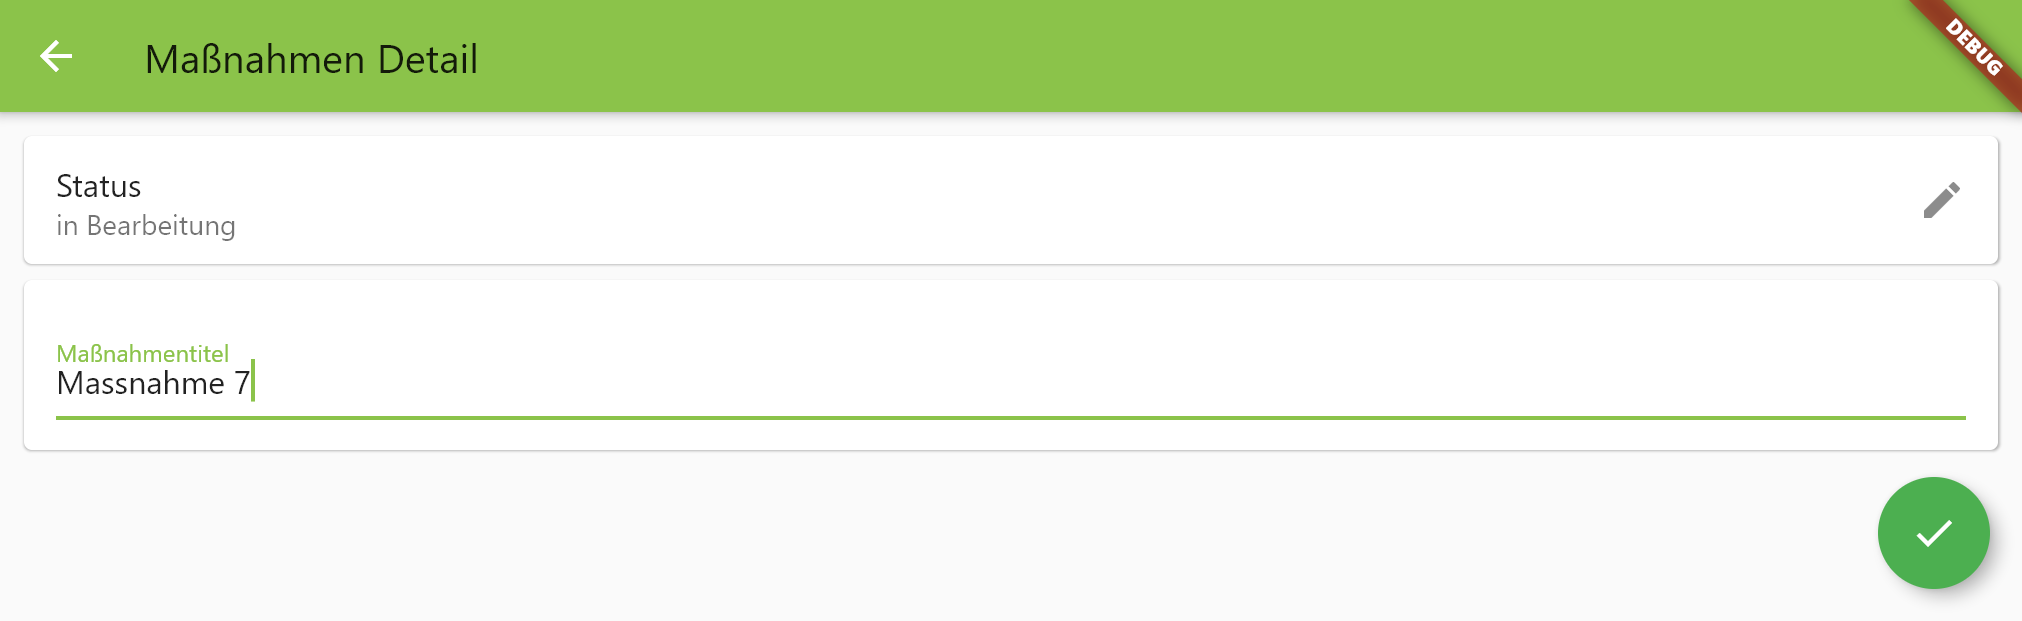
\includegraphics[width=1.0\textwidth]{Inhalt/Hauptteil/Implementierung/Schritt-1/Eingabemaske.png}
  \caption[Schritt 1 Eingabemaske]{Die Eingabemaske zeigt im Schritt 1 eine Karte zum Selektieren des Status und ein Eingabefeld für den Titel. Quelle: Eigene Abbildung}
  \label{fig:Schritt1Eingabemaske}
\end{figure}
Sie ermöglicht die Eingabe des Maßnahmen-Titels über ein simples Eingabefeld. Darüber hinaus ist die Selektions-Karte für den Status zu sehen. Mit einem Klick auf diese Karte öffnet sich der Selektions-Bildschirm. Er ermöglicht die Auswahl der Auswahloptionen, in diesem Fall die Optionen \enquote{in Bearbeitung} und \enquote{abgeschlossen}
\Abb{\ref{fig:Schritt1SelektionsBildschirmStatus}}.

\begin{figure}[H]
  \centering
  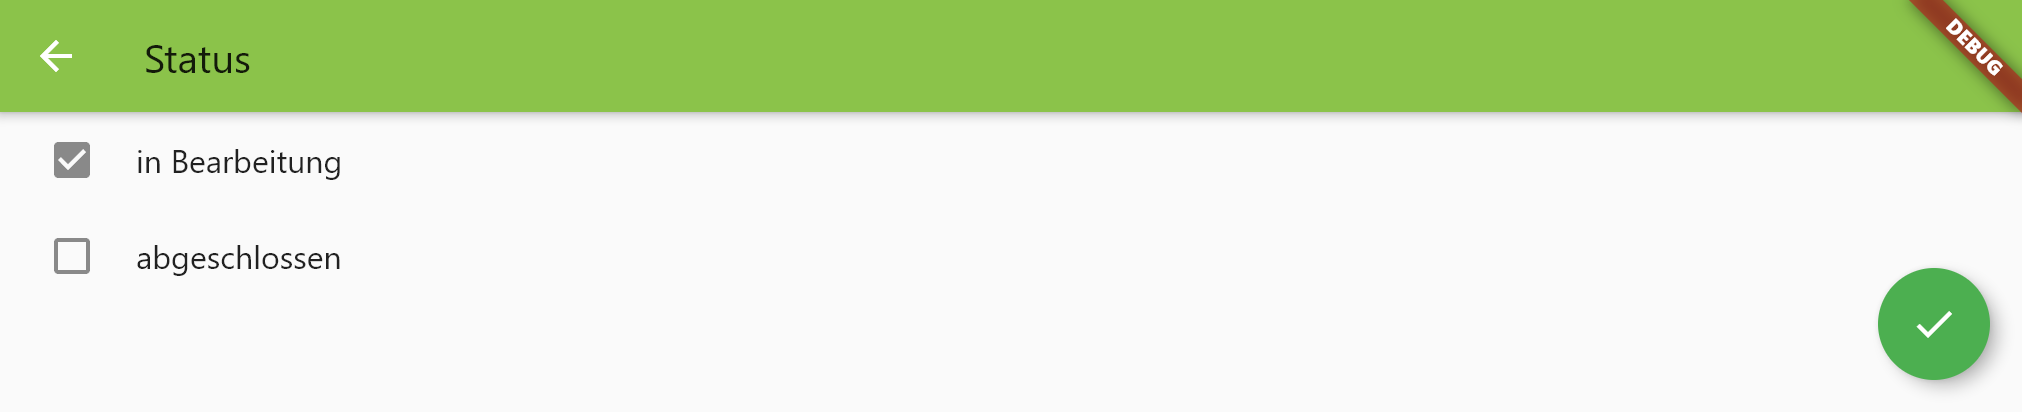
\includegraphics[width=1.0\textwidth]{Inhalt/Hauptteil/Implementierung/Schritt-1/Status Auswahl.png}
  \caption[Schritt 1 Selektions-Bildschirm für Status]{Der Selektions-Bildschirm für das Feld Status erlaubt die Auswahl der Optionen \enquote{in Bearbeitung} und \enquote{abgeschlossen}. Quelle: Eigene Abbildung}
  \label{fig:Schritt1SelektionsBildschirmStatus}
\end{figure}

% TODO: rausgekürzt, doch wieder rein nehmen?
%\footnoteI{Ein floating action button (FAB) ist im Material Design ein Button, der über der Benutzeroberfläche schwebt und daher dem Benutzer leicht ins Auge fällt. Aus diesem Grund wird er für primäre Aktionen genutzt - in diesem Fall dem Erstellen einer neuen Maßnahme. \footnote{\cite{MaterialDesignFloatingActionButton}}} ist in der unteren rechten Ecke der Ansicht zu finden. Mit einem Klick darauf wird der Benutzer auf die zweite Ansicht weitergeleitet: die Eingabemaske. 

\subsubsection{Auswahloptionen hinzufügen}

Dart verfügt – anders als beispielsweise Java\footcite[Vgl.][S. 321]{TheJavaLanguageSpecificationJavaSE16Edition} – nicht über Aufzählungstypen mit zusätzlichen Eigenschaften. Das Schlüsselwort \mintinline{dart}{enum} in Dart erlaubt lediglich die Auflistung konstanter Symbole\footcite[Vgl.][S. 74f.]{DartProgrammingLanguageSpecification5thedition}. Für die Auswahl Optionen ist es jedoch notwendig, dass es zwei Eigenschaften gibt:
\begin{itemize}
  \parsep 0pt
  \topsep 0pt
  \itemsep 0pt

  \item die Abkürzung, die in der resultierendem Datei gespeichert werden soll
  \item und der Beschreibungstext, welcher in der Oberfläche angezeigt wird.
\end{itemize}
Das hat den Hintergrund, dass die Abkürzungen weniger Speicherplatz einnehmen und die Beschreibung sich in Zukunft auch ändern darf. Würde anstatt der Abkürzung die Beschreibung als Schlüssel verwendet werden, so würde eine Datei, die mit einer älteren Version des Formulars erstellt wurde, nicht mehr von neueren Versionen der Applikationeingelesen werden können. Der alte Beschreibungstext würde nicht mehr mit dem Text übereinstimmen, der als Schlüssel in der Anwendung verwendet wird.


Die beiden Zustände \enquote{in Bearbeitung} und \enquote{abgeschlossen} werden daher in Listing \ref{Schritt1KlasseLetzterStatus} als statische Klassenvariablen deklariert \Z{6-7}. Die beiden Konstruktor-Aufrufe übergeben dabei als erstes Argument die Abkürzung und als zweites Argument die Beschreibung. Der Konstruktor selbst \Z{9-10} deklariert die beiden Parameter als positionale Parameter.

\begin{alexlisting}{Schritt 1}{Die Klasse LetzterStatus}
  {Quellcode/Schritt-1/conditional_form/lib/choices/choices.dart}
  {firstline=5, lastline=11}
  \label{lst:Schritt1KlasseLetzterStatus}
\end{alexlisting}

\paragraph{Positionale Parameter}

Im Vergleich zu den benannten Parametern ist bei den positionalen Parametern nur ihre Reihenfolge in der Parameterliste ausschlaggebend. Das Argument für die \IC{abbreviation} steht dabei also immer an erster Stelle und das Argument für \IC{description} immer an der zweiten \Z{6-7}. Positionale Parameter sind vorgeschrieben. Werden sie ausgelassen, so gibt es einen Compilerfehler. \DartSpec{74f.}

Die Klasse \IC{LetzterStatus} erbt von der Basisklasse \IC{Choice} \Z{5}. Der Konstruktor der Klasse \Z{9} übergibt beide Parameter als Argumente an den Konstruktor der Klasse \IC{Choice}. Genau wie in Java wird mithilfe des Schlüsselwortes \IC{super}\Z{10} der Konstruktor der Basisklasse aufgerufen. Doch anders als in Java erfolgt der Aufruf des super Konstruktors nicht in der ersten Zeile des Konstruktor-Körpers \JavaSpec{310}. Weil das Aufrufen des Konstruktors der Basisklasse zum statischen Teil der Objekt-Instanziierung gehört, muss der Aufruf von \IC{super} in der Initialisierungsliste erfolgen. Die Initialisierungsliste wird mit dem \IC{:} nach der Parameterliste eingeleitet \Z{10}\DartSpec{42}.

Die Basisklasse \IC{Choice} \Lst{\ref{lst:Schritt1KlasseChoice}} deklariert lediglich die beiden Felder \IC{description} und \IC{abbreviation} jeweils als \IC{String} \Z{4-5}. Beide sind mit \IC{final} gekennzeichnet, was sie zu unveränderlichen Instanzvariablen macht. Nach der Initialisierung, können sie keine anderen Werte annehmen. \DartSpec{S16} Die Initialisierung der beiden Variablen muss im statischen Kontext der Instanziierung erfolgen. Mit der abgekürzten Schreibweise \IC{this.abbreviation} und \IC{this} \IC{.description} im Konstruktor \Z{7} werden die Parameter den Feldern zugewiesen.

\begin{alexlisting}{Schritt 1}{Die Klasse Choice}
  {Quellcode/Schritt-1/conditional_form/lib/choices/base/choice.dart}
  {firstline=3, lastline=7}
  \label{lst:Schritt1KlasseChoice}
\end{alexlisting}

Dies erübrigt sowohl die Angabe des Parametertypes mittels \IC{(String abbreviation, String description)}, denn der Typ des Parameters kann bereits durch Angabe des Typs in der Instanzvariablen-Deklaration\Z{4-5} abgeleitet werden. Außerdem entfällt auch die Zuweisung, die man ansonstenin der Form \IC{this.abbreviation = abbreviation} und \IC{this.}\IC{description = description} in der Initialisierungsliste erreichen würde.\DartSpec{40f}
% Auch String description wird gespart


\begin{alexlisting}{Schritt 1}{Die Menge letzterStatusChoices}
  {Quellcode/Schritt-1/conditional_form/lib/choices/choices.dart}
  {firstline=13}
  \label{lst:Schritt1DieMengeLetzterStatusChoices}
\end{alexlisting}

Die Variable \IC{letzterStatusChoices} fasst die beiden statischen Klassenvariablen als eine Kollektion zusammen. Da es sich um eine solche Kollektion handelt, in der jedes Element nur ein einziges Mal vorkommen darf, ist hier von einer Menge zu sprechen. Auffällig hier ist, dass das Schlüsselwort new fehlt. In Dart ist das Schlüsselwort für die Konstruktion von Instanzen optional.  Die Klasse, die zur Konstruktion dieser Menge verwendet wird, ist die selbst erstellte Klasse choices. Über das Typargument LetzterStatus wird erreicht, das ausschließlich Variablen  dieses Typs in der Menge eingefügt werden dürfen. Wird stattdessen eine Variable eingefügt, die weder vom selben Typ, noch von einem Typ, der von letzter Status erbt, so gibt es einen Compilerfehler. Dies dient einzig und allein dem Zweck, dem  Fehler vorzubeugen, dass aus Versehen falsche Optionen in der Menge eingetragen werden. Über den Parameter name ist es möglich dieser Menge die Beschriftung “Status” hinzuzufügen.  Es handelt sich hier um einen  benamten Parameter.

Listing 4 zeigt die Klasse choices. Sie erbt von UnmodifiableSetView und erlaubt damit die Erstellung  einer eigenen Menge - auch Set genannt. Methoden, die man von einem Set erwartet,  lassen sich somit direkt auf  Instanzen der Klasse Choices aufrufen. Darunter unter anderem die contains Methode,  welche erlaubt, das Vorhandensein eines Objektes im Set zu überprüfen.
%   todo Referenz contains einfügen
%    todo Referenz UnmodifiableSetView
Instanzvariable name -  deklariert in Zeile 11 - wird im Konstruktor in Zeile 16 zugewiesen. Auffällig hierbei ist, dass der Parameter in geschweiften Klammern geschrieben steht und das Schlüsselwort required  vorangestellt ist. Das macht den Parameter zu einem vorgeschriebenen benannten Parameter.

\paragraph{Vorgeschriebene benamte Parameter}

Gewöhnlicher benannte Parameter sind optional. Wird ihnen das Schlüsselwort \IC{required} vorangestellt, so müssen sie gesetz werden, denn sonst gibt es einen Compilerfehler.  An dieser Stelle ist das \IC{required} Schlüsselwort sinnvoll, denn es handelt sich um den Datentyp String der nicht den  wert \IC{null} annehmender. Würde  der Parameter aber optional sein, so wäre es möglich, das programm zu kompilieren, auch wenn bei Aufrufen des Konstruktors kein Argument für den Parameter übergeben wurde. Doch in diesem Fall gäbe es keinen Initialwert für Name und somit müsste der  Instanzvariable null  zugewiesen werden. in der statischen Analyse wird daher sichergestellt, das Instanzvariablen durch benannte Parameter nur dann initialisiert werden dürfen, wenn dieser durch required  als vorgeschrieben gekennzeichnet sind und damit unter keinem Umstand ausgelassen werden können. Dürfte name den Wert Null annehmen, So würde es sich um den nullable Datentyp String  mit der Notation String? Handeln.

\paragraph{Typen ohne NULL-Zulässigkeit} Im Vergleich zu vielen anderen Programmiersprachen wie beispielsweise in Java wird in Dart zwischen gewöhnlichen Typen und nullable Typen unterschieden. In Sprachen wie Beispielsweise Java ist es nur bei atomaren Datentypen wie int und float vorgeschrieben einen Wert anzugeben. Null ist bei diesen primitiven Datentypen nicht als Wert erlaubt. Doch nicht atomare Datentypen erlauben immer die Angabe von Null als wert. Null drückt dabei immer das Nichtvorhandensein von Daten aus. Ab Dart 2.12   kann allen Datentypen standardmäßig keinen neuen Wert zugewiesen werden.  das hat den Vorteil, dass der Compiler sich darauf verlassen kann, das eine Variable niemals den Wert 0 haben kann. Das ist besonders dann nützlich, wenn auf  Einem Objekt eine Methode aufgerufen wird. Ist die Referenz das Objekt ist in Wahrheit 0 so gibt es erst zur Laufzeit einen Fehler, dass die Methode auf der Referenz \IC{null}nicht aufgerufen werden kann. Damit  ein Laufzeitfehler geworfen werden kann, muss vor jedem Aufruf einer Methode auf einer Referenz überprüft werden, ob die Referenzen nicht \IC{null} sind. Würde diese Überprüfung nicht stattfinden, so  könnte kein Laufzeitfehler geworfen werden und das Programm würde ohne Fehlermeldung abstürzen. Handelt es sich allerdings um eine Referenz, die niemals den Wert 0 annehmen kann, so kann der Compiler die Überprüfung auf 0 Wörter für diese Referenzen überspringen. Damit hört zusätzlich die Ausführungsgeschwindigkeit erhöht, da die  Überprüfung auf \IC{null}Zeit in Anspruch nimmt. Vor allem aber ist das forderheft für den Wickler, da der Compiler  Fehlermeldungen und Warnungen mitteilen kann, wenn  Operationen  mit Variablen mit potenziellen \IC{null}  Werten verwendet werden.

Neben Name wird mit  choiceByAbbreviation eine weitere Instanzvariable deklariert 12.
es handelt sich um den Datentyp map -  eine Kollektion die Daten mittels Schlüssel Wertepaaren ablegen kann.   als Schlüssel wird  die Abkürzung mit dem Datentyp String verwendet. Als wert ist der  generische typ Parameter t angegeben.  der typ Parameter ist in Zeile zehn deklariert und muss  mindestens von der Klasse Joyce erben. In choiceByAbbreviation werden also die Auswahlmöglichkeiten über  ihre Abkürzung abgelegt und können über dieselbe wieder referenziert werden.  Da es sich auch hier um eine unveränderliche Instanzvariable handelt, muss sie schon in der Initialisierungsliste initialisiert werden 17 bis 19. Dabei wird zunächst mit der öffnenden geschweiften Klammer 17 ein sogenanntes Map Literal begonnen, welches mit  schließenden geschweiften Klammer 19 endet.

\paragraph{Set und Map Literale}

Dart erlaubt es  setz und Maps als sogenannte literale zu deklarieren. es entfällt also die Instanziierung eines Sets oder einer Map über den Klassennamen und der darauffolgenden Zuweisung der einzelnen Werte. Stattdessen startet das literal mit einer öffnenden geschweiften Klammer und endet mit einer  schließenden geschweiften Klammer Punkt innerhalb der Klammern werden die Werte im Fall eines Sets  mit, getrennt nacheinander aufgeführt. Im Fall einer Map werden der Schlüssel und der Wert durch einen : voneinander getrennt und die Schlüsse Wertepaare wiederum durch, getrennt nacheinander aufgelistet.

Auffällig ist jedoch, dass In Zeile 18 dem Set lateral keine  einfache Auflistung von Werten übergeben wird. Stattdessen wird das mit dem sogenannte collection for eine wiederholung verwendet.

\paragraph{Collection for} Dart erlaubt es Schleifen innerhalb von Listen-, Set- und Map-Literalen zu verwenden. Dabei darf die Schleife jedoch keinen steifen Körper besitzen. Ledig der Schleifenkopf wird dazu in das literal selbstgeschrieben gefolgt von dem Wert, der bei jedem Schleifendurchlauf  dem literal hinzugefügt werden soll. Da wir kann der Wert von der Schleifen variable abgeleitet werden.  In Zeile 18 wird beispielsweise durch die  Menge aller Auswahloptionen choices iteriert und dabei in jedem Schleifendurchlauf  die Ausweise Option in die Variablen choice gespeichert. Während des Schleifendurchlauf wird dann ein Wertepaar gebildet wobei choice.abbreviation der Schlüssel ist und Das Objekt choice selbst  der Wert.

Die Map choiceByAbbreviation erlaubt es nach der Initialisierung mit Hilfe der Methode fromAbbreviation 14 über die Abkürzung das dazugehörigen Choice Objekt abzurufen. Beispielsweise gibt der Befehl letzterStatusChoices.fromAbbreviation(“fertig”) das Objekt LetzterStatus("fertig", "abgeschlossen")  zurück. Auffällig dabei ist das der Parameter abbreviation Mit dem Typen String? und der generische Rückgabetyp mit T? gekennzeichnet ist. Der Suffix ? macht beide zu Typen mit Null-Zulässigkeit.

\paragraph{Typen mit NULL-Zulässigkeit}

Wird in Dart hinter einem Typen ein \IC{?} Angegeben, so kann die Variable nicht nur  Werte annehmen, die dieser Datentyp zulässt sondern zusätzlich auch noch den Wert 0, der  ausdrückt, dass die Variable keinen Wert hat. Methoden auf Objekten mit nur Zulässigkeit aufzurufen ist nicht ohne weiteres möglich.  Der wird aus  solange nicht durch eine Fallunterscheidung zuvor überprüft wird, dass die Variable tatsächlich nicht \IC{null} ist oder der Aufruf der Methode  mit dem Suffix !  nach dem Objekt erzwungen wird.
% Todo high prio rferenz einfügen

Die Methode fromAbbreviation Soll für die Deserialisierung genutzt werden.  sollten in Formular Auswahlfelder leer gelassen worden sein, so haben  entsprechenden variablen den Wert \IC{null}. Wenn nun das Formular abgespeichert wird, so tauchen auch in der abgespeicherten json-datei keine  Werte für das fällt auf. Wird die Dateiendung gelesen wird die Methode fromAbbreviation  genutzt um aus der in der json-datei gespeicherten Abkürzung wieder die entsprechende Auswahl Option abzurufen.  Sollte jedoch kein Wert hinterlegt sein so wird \IC{letzterStatusChoices.fromAbbreviation(null)} aufgerufen werden. Dadurch wird klar, dass der Parameter \IC{null} zulassen muss. Es impliziert auch, dass potenziell \IC{null} zurückgeben werden kann, da für den Schlüssel \IC{null} kein Wert in der Map hinterlegt sein kann. Deshalb  erlaubt auch der Rückgabetyp \IC{null}-Werte.




\begin{alexlisting}{Schritt 1}{Die Klasse Choices}
  {Quellcode/Schritt-1/conditional_form/lib/choices/base/choice.dart}
  {firstline=10}
  \label{lst:Schritt1KlasseChoices}
\end{alexlisting}

\subsubsection{Serialisierung einer Maßnahme}

Damit die Daten angezeigt und verändert werden können, müssen sie zunächst serialisierbar sein, sodass sie auf einen Datenträger geschrieben und von dort auch wieder gelesen werden können.
% todo: Serialisierung erklären
Die zwei bekanntesten Bibliotheken zum Serialisieren in Dart heißen json_serializable und built_value.
% todo medium: Vgl. https://flutter.dev/docs/development/data-and-backend/json
% todo medium: Was ist flutter, Flutter nutzt Dart
% todo medium: Model View View Model
Beide haben gemeinsam, dass sie Quellcode generieren, welcher die Umwandlung der Objekte in JSON übernimmt.
% todo: json_serializable erklären
% todo: tree shaking erklären https://flutter.dev/docs/development/data-and-backend/json
built_value bietet im Gegensatz zu JSON Serializable jedoch die Möglichkeit unveränderbare Werte-Typen -  sogenannte immutable value types -  zu erstellen. Da diese  unveränderbaren Werte noch bei der Erstellung des sogenannten ViewModels -  Mehr dazu im Kapitel XXX - hilfreich werden, wurde sich für diese Bibliothek entschieden.
% todo high: Kapitel Referenz einfügen

Ein Werte-Typ für built_value erfordert etwas Boilerplate-Code,  um den generierten Quellcode mit der selbstgeschriebenen Klasse zu verknüpfen.  
Entwicklungsumgebungen wie Visual Studio Code und Android Studio erlauben solchen Boilerplate Code generieren zu lassen und dabei nur die erforderlichen Platzhalter einzugeben.
In Visual Studio Code werden diese Templates \enquote{Snippets} genannt, in Android Studio heißen sie \enquote{Live Templates}.  Listing \ref{lst:BuiltValueLiveTemplate} zeigt, wie das live Template für das Generieren eines Wertetyps  für built_value aussieht. Templates für built_value wie dieses und weitere müssen nicht vom Nutzer eingegeben werden, sondern existieren bereits als Plugin für die beiden Entwicklungsumgebungen\footnoteL{https://plugins.jetbrains.com/plugin/13786-built-value-snippets}, \footnoteL{https://marketplace.visualstudio.com/items?itemName=GiancarloCode.built-value-snippets}.


% todo medium: live template erklären
% todo ask medium: Kein Autor, nur git Name
% todo ask medium: Quelle nötig?

\begin{listing}[h]
  \begin{minted}[firstnumber=6]{dart}
part '$file_name$.g.dart';

abstract class $ClassName$ implements Built<$ClassName$, $ClassName$Builder> {
    $todo$
    
    $ClassName$._();
    factory $ClassName$([void Function($ClassName$Builder) updates]) = _$$$ClassName$;
}
\end{minted}
  \caption[built_value Live Template]{Live Template für die Erstellung von built_value Boilerplate-Code in Android Studio, Quelle: Jetbrains Marketplace Built Value Snippets Plugin}
  \label{lst:BuiltValueLiveTemplate}
\end{listing}

\IC{\$ClassName\$} Wird dabei jeweils durch den gewünschten Klassennamen ersetzt. Android Studio erlaubt, dass bei Einfügen des live templates der Klassenname einmalig eingegeben werden muss.  Anschließend wird mithilfe des live templates der Boilerplate Code generiert.

In Listing \ref{lst:Schritt1WerteTypMassnahme} ist der Werte-Typ \IC{Massnahme} zu sehen. Die Zeilen 11 bis 13, sowie 23 bis 28 wurden dabei automatisch erstellt. Die Zeilen 14 bis 21 wurden hinzugefügt. Zunächst soll die Maßnahme über die \IC{guid} eindeutig identifiziert werden können.

\begin{alexlisting}{Schritt 1}{Der Werte-Typ Massnahme}
  {Quellcode/Schritt-1/conditional_form/lib/data_model/massnahme.dart}
  {firstline=6, lastline=23}
  \label{lst:Schritt1WerteTypMassnahme}
\end{alexlisting}

\paragraph{Globally Unique Identifier} 
Ein GUID – Kurzform von Globally Unique IDentifier – ist  eine Folge von 128 Bits, die zur Identifikation genutzt werden kann. Eine solche GUID hat einer textuelle Repräsentation wie beispielsweise die folgende: \IC{'f81d4fae-7dec-11d0-a765-00a0c91e6bf6'}


%  todo - guid General unique identifier erklären
Die Attribute \IC{letzteBearbeitung} und \IC{identifikatoren} sind im Gegensatz zu dem String-Attribut guid zusammengesetzte Datentypen, die im Folgenden weiter beleuchtet werden.

Auffällig ist, dass es sich hier um eine abstrakte Klasse handelt und die drei Attribute jeweils Getter-Methoden ohne Implementierung sind. Eine solche Getter-Methode speichert keinen wert, sondern gibt lediglich den Wert eines Feldes zurück. Die dazugehörigen Felder,  Setter-Methoden, die konkrete Klasse und der restliche generierte Code ist in der gleichnamigen Datei mit der Endung \IC{.g.dart} (Zeile 11) zu finden.

Die Klassen-Methode \IC{_initializeBuilder} kann in jedem Werte-Typ hinterlegt werden, um Standardwerte für Felder festzulegen.
% todo medium: Vgl. https://pub.dev/packages/built_value/changelog
Die Methode wird intern von \enquote{built_value} aufgerufen. Bei dem Feld \enquote{guid} handelt es sich um einen String, der keine Null-Werte zulässt. Könnte das Feld auch Null-Werte annehmen, so wäre die Notation in Dart dafür stattdessen \IC{String? get guid;}. \enquote{built_value} erwartet also immer einen Wert für dieses Feld. Sollte die Datei gelesen werden, welche die Maßnahmen enthält, so enthält jede Maßnahme bei der Deserialisierung den abgespeicherten Wert für die \IC{guid} und somit wird das Feld gefüllt. Doch sollte eine leere Maßnahme über einen Konstruktor erstellt werden, so wäre das Feld \enquote{guid} leer und \enquote{built_value} würde einen Fehler auslösen. Aus diesem Grund wird in der Zeile 21 für das Feld \IC{guid} ein Standardwert festgelegt, nämlich eine zufällige generierte ID die dem Standard Uuid der Version 4 entspricht.
% todo high:  https://www.ietf.org/rfc/rfc4122.txt
Zu diesem Zweck wird das Builder-Objekt verwendet. Die Klasse \IC{MassnahmeBuilder} gehört dabei zu dem von \enquote{built_value} generierten Quellcode. Der Parametername wird hier – wie so häufig im builder pattern – mit einem b für Builder abgekürzt. Die Syntax \IC{=>} leitet  einen sogenannten \enquote{arrow function body} ein. Dabei handelt es sich schlicht um einen Funktions-Körper, der genau eine Anweisung ausführt und deshalb nicht in öffnenden und schließenden geschweiften Klammern gesetzt werden muss.\DartSpec{18f., 234} 
Auf dem Bilder-Objekt können dann die Eigenschaften so gesetzt werden, als wären sie die Eigenschaften von dem Objekt \IC{Massnahme}. In Wahrheit werden sie aber nur auf den Builder-Objekt angewendet.  Ebenfalls auffällig ist die Syntax \IC{b..guid}.  Statt dem Punkt zum Zugriff auf Attribute des Objektes wird hier der sogenannte Kaskadierungs-Operator benutzt.

\paragraph{Der Kaskadierungs-Operator}

Durch Eingabe von zwei aufeinanderfolgende Punkten \IC{..} statt nur einem \IC{.} können mehrere Operationen an einem Objekt ausgeführt werden, ohne  das Objekt zuvor einer Variable Zuzuweisen oder die Operationen über dessen Namen wiederholt aufzurufen.\DartSpec{149f.} Beispiel: die Aufrufe \IC{objekt.tueEtwas();} \IC{objekt.tueEtwasAnderes();} und \IC{objekt..tueEtwas()..tueEtwasAnderes();} sind äquivalent. 

Da der Kaskadierung-Operator jedoch dazu verwendet wird, mehrere Operationen auf einem Objekt auszuführen, hat er in Zeile 16 keine Funktion. Doch bei Änderung eines Objektes über das builder pattern werden für gewöhnlich mehrere Operationen am gleichen Builder Objekt ausgeführt, weshalb - der Stringenz halber - der Kaskadierung-Operator immer  im Zusammenhang mit dem Bilder Objekt verwendet wird. 

Die Attribute \IC{letzteBearbeitung} und \IC{identifikatoren} \Z{11, 13} erhalten dagegen ganz automatisch Standardwerte in Form von Instanzen der dazugehörigen Klassen. Diese wiederum konfigurieren ihre eigenen Felder und deren initialen Werte.



Der Werte-Typ \IC{Identifikatoren} ist in Listing \ref{lst:Schritt1WerteTypIdentifikatoren} zu sehen. Er enthält das Attribut \IC{massnahmenTitel}, welcher im Eingabeformular durch das Texteingabefeld gefüllt werden wird.

\begin{alexlisting}{Schritt 1}{Der Werte-Typ Identifikatoren}
  {Quellcode/Schritt-1/conditional_form/lib/data_model/massnahme.dart}
  {firstline=25, lastline=30}
  \label{lst:Schritt1WerteTypIdentifikatoren}
\end{alexlisting}

Schließlich enthält der Werte-Typ \IC{LetzteBearbeitung} in Listing \ref{lst:Schritt1WerteTypLetzteBearbeitung} noch die Attribute \IC{letztesBearbeitungsDatum} in Zeile 43 und \IC{letzterStatus} in Zeile 50. Im Eingabeformular wird der Selektions-Bildschirm den Inhalt des Feldes \IC{letzterStatus} Bestimmen. Der initiale Wert auf wird in Zeile 54 auf einen konstanten Wert gesetzt, der dem Zustand \IC{'in Bearbeitung'} entspricht - mehr dazu im Kapitel \HP{Kapitel einfügen}.
% todo high: Kapitel Choices einfügen

\begin{alexlisting}{Schritt 1}{Der Werte-Typ LetzteBearbeitung}
  {Quellcode/Schritt-1/conditional_form/lib/data_model/massnahme.dart}
  {firstline=41, lastline=54}
  \label{lst:Schritt1WerteTypLetzteBearbeitung}
\end{alexlisting}

Das Attribut \IC{letztesBearbeitungsDatum} ist dagegen nicht im Formular änderbar, sondern wird einmalig in Zeile 53 auf den aktuellen Zeitstempel gesetzt. Zugehörig zu diesem Attribut gibt es noch eine abgeleitete Eigenschaft namens \IC{formattedDate} \Z{45-48}.  Es ist eine Hilfsmethode, die das letzte Bearbeitungsdatum in ein für Menschen lesbares Datumsformat umwandelt. In dem Übersichts-Bildschirm Abbildung \ref{fig:Schritt1Uebersicht} ist das Datumsformat sichtbar.

Da diese Getter-Methode eine Implementierung besitzt, wird für sie von \enquote{built_value} kein Quellcode für die Serialisierung generiert.

Bevor die Werte-Typen serialisiert werden können, muss built_value jedoch noch mitgeteilt werden, für welche Werte-Typen Serialisierungs-Funktionen generiert werden sollen. Dazu werden über die Annotation \IC{@SerializersFor} die gewünschten Klassen aufgelistet \LstZ{\ref{lst:Schritt1Serialisierer}}{10}. Die Zeilen 11 und 12 sind dabei immer gleich, es sei denn, es ist ein anderer Serialisierung Algorithmus gewünscht. In diesem Fall wird das \IC{StandardJsonPlugin}verwendet. 

\begin{alexlisting}{Schritt 1}{Der Serialisierer für Massnahme und Storage}
  {Quellcode/Schritt-1/conditional_form/lib/data_model/serializers.dart}
  {firstline=10, lastline=12}
  \label{lst:Schritt1Serialisierer}
\end{alexlisting}


% Storage Klasse zeigen und beschreiben
% serializers Klasse zeigen und beschreiben
% Korrigieren (Unten)
Wird nun der Befehl  \IC{flutter pub run build_runner build} ausgeführt, so wird der Quellcode generiert und die Werte-Typen können für die Serialisierung genutzt werden.

\subsubsection{Test der Serialisierung einer Maßnahme}

Das Ergebnis der Serialisierung wird im dazugehörigen Unit-Test ersichtlich \Lst{\ref{lst:SerialisierungEinerMassnahmeUnittest}}.
In Zeile 8 wird ein Objekt der Klasse \IC{Massnahme} instanzieiert. Anders als bei gewöhnlichen Datentypen lassen sich bei diesem unveränderlichen Datentyp keine Attribute nach der Erstellung anpassen. Die einzige Möglichkeit besteht darin, ein neues Objekt  mit dem gewünschten Attributwert zu erstellen und die restlichen Werte des alten Objektes zu übernehmen. Dies ist mit Hilfe des sogenannten Builder-Entwurfsmuster es möglich, welches in built_value Anwendung findet. 

\paragraph{Erbauer-Entwurfsmuster} Das Erbauer-Entwurfsmuster - englisch builder pattern - ist ein Erzeugungsmuster, welches die Konstruktion komplexer Objekte von ihrer Repräsentation trennt. Es gehört zu der Serie von Entwurfsmustern der Gang of Four. \footcite[Vgl.][S. 119]{gamma2009entwurfsmuster}. Im Fall von built_value trennt es die unveränderlichen Objekte von ihrer Konstruktion. Über den Builder lassen sich Änderungen an diesen unveränderlichen Objekten vornehmen, wodurch eine Kopie dieses unveränderlichen Objekt mit der gewünschten Änderung, zurückgegeben wird.

In den Zeilen 9 bis 10 wird so ein neues Objekt von der Klasse Maßnahme mit Hilfe der Methode \IC{rebuild} erzeugt und anschließend der Referenz \IC{massnahme} zugewiesen, wodurch sie ihren alten Wert verliert. Über die generiertet Methode \IC{serializers} \IC{.serializeWith} kann das Objekt in Json übersetzt werden. Der erste Parameter \IC{Massnahme.serializer} gibt dabei an, wie diese Serialisierung erfolgen soll und auch dieses Objekt wurde von \enquote{built_value} generiert. Der zweite Parameter ist die tatsächliche \IC{massnahme}, die in Json umgewandelt werden soll. Die Zeilen 13 bis 21 erstellen das Json Dokument, mit dem das serialisierte Ergebnis am Ende verglichen werden soll. Dabei werden die gleichen Eigenschaften eingetragen. So etwa die \IC{guid}\Z{14}, welcher bei der Initialisierung der Maßnahme automatisch und zufällig erstellt wurde. Außerdem das letzte Bearbeitungsdatum, welches den Zeitstempel erhält, zudem die Maßnahme generiert wurde. Da built_value bei der Serialisierung die Datumswerte in Mikrosekunden umwandelt, muss für das erwartete Json-Dokument das gleiche passieren \Z{16-17}. Der \IC{'letzterStatus'} \Z{18} wird hierbei auf den Standardwert \IC{'bearb'} gesetzt und der \IC{'massnahmenTitel'} \Z{20} auf den gleichen Wert, der in Zeile 9 übergeben wurde. 
Schließlich vergleicht die Methode \IC{expect} das tatsächlich serialisierter Json-Dokument mit dem, welches zuvor zum Vergleich aufgebaut wurde. Der zweite Parameter ist ein sogenannter \IC{Matcher} und die Variante mit dem Namen \IC{equals} überprüft auf absolute Gleichheit. 

\begin{alexlisting}{Schritt 1}{Serialisierung einer Maßnahme Unittest}
  {Quellcode/Schritt-1/conditional_form/test/data_model/massnahme_test.dart}
  {firstline=6, lastline=23}
  \label{lst:SerialisierungEinerMassnahmeUnittest}
\end{alexlisting}

Analog zur Serialisierung testet der Unit-Test in Listing \ref{lst:DeserialisierungEinerMassnahmeUnittest} auch die Deserialisierung. Das Json-Dokument ist dabei sehr ähnlich und unterscheidet sich lediglich in zwei Details. Der \IC{'guid'} wird auf einen festen Wert festgelegt \Z{38}, statt - wie zuvor - durch den in dem Initialisierungs-Prozess der Maßnahme zufällig generiert zu werden. Außerdem wird auch das \IC{letztesBearbeitungsDatum} festgesetzt, nämlich auf die Microsekunde \IC{0} \Z{40}. 

\begin{alexlisting}{Schritt 1}{Deserialisierung einer Maßnahme Unittest}
  {Quellcode/Schritt-1/conditional_form/test/data_model/massnahme_test.dart}
  {firstline=36, lastline=56}
  \label{lst:DeserialisierungEinerMassnahmeUnittest}
\end{alexlisting}


Zum Vergleich wird in den Zeilen 46 bis 52 eine Maßnahme über das Builder-Entwurfsmuster generiert und die gleichen feste Werte werden für die Eigenschaften übergeben. 
Dabei ist darauf zu achten, dass die Instanzvariable \IC{letzteBearbeitung} keinen Wert über den Zuweisungs-Operator \IC{=} erhält, sondern stattdessen die Methode \IC{update} darauf aufgerufen wird.

Da es sich bei der Instanzvariable \IC{letzteBearbeitung} genauso um ein Object eines Wertetypen - handelt, ist sie ebenso unveränderlich. Deshalb kann sie nur über einen Builder manipuliert werden. Ein Blick in den generierten Quellcode offenbart, dass es sich in Wahrheit um einen Bilder handelt \LstZ{\label{lst:Schritt1InstanzvariableLetzteBearbeitungGibtEinenLetzteBearbeitungBuilderZurueck}}{224-225}.

\begin{alexlisting}{Schritt 1}{Instanzvariable \IC{letzteBearbeitung} gibt einen \IC{LetzteBearbeitungBuilder} zurück}
  {Quellcode/Schritt-1/conditional_form/lib/data_model/massnahme.g.dart}
  {firstline=216, lastline=227} 
  \label{lst:Schritt1InstanzvariableLetzteBearbeitungGibtEinenLetzteBearbeitungBuilderZurueck}
\end{alexlisting}

Außerdem müssen die Microsekunden für das Datum zunächst in ein Objekt von \IC{DateTime} umgewandelt werden muss. Dafür wird der benahmte Konstruktor \IC{DateTime} \IC{.fromMillisecondsSinceEpoch} \Z{51} aufgerufen.

\paragraph{Benanmte Konstruktoren} In Programmiersprachen wie beispielsweise Java können Methoden überladen werden, indem ihre Methodensignatur geändert wird. Beim Aufruf der Methode kann über die Anzahl und die Typen der übergebenen Argumente die gewünschte Methode gewählt werden. Das gleiche gilt für Konstruktoren. Wird ein weiterer Konstruktor für eine Klasse in Java benötigt, so besteht einzig und allein die Möglichkeit darin, den Konstruktor zu überladen. Sowohl überladene Methoden als auch überladene Konstruktoren existieren in Dart nicht. Wird also in dartein Alternative constructorgewünscht Komma so muss er einen Namen bekommen. Beim Aufruf des Konstruktors wird dieser Name dann mit einem \IC{.} nach dem Klassennamen angegeben, um den gewünschten Konstruktor zu benennen.


Ganz ähnlich wie bei der Serialisierung wird nun mit dem Befehl \IC{serializers} \IC{.} \IC{deserializeWith} unter Angabe des Objektes, welches die Deserialisierung übernehmen soll - nämlich wiederum \IC{Massnahme.serializer} - das Json-Dokument in ein Objekt das Werte-Typs \IC{Massnahme} deserialisiert \Z{53-54}. Schließlichh wird in Zeile 56 das Ergebnis der Deserialisierung mit dem gewünschten Ergebnis verglichen.

 

Gibt man in der Kommandozeile den Befehl \IC{flutter} \IC{test} \IC{test}\IC{/data_model}\IC{/massnahme _test.dart} ein, so werden die Tests in der Testdatei ausgeführt. Die Ausgabe \IC{00:01 +2: All tests passed!} teilt mit, dass beide Tests ausgeführt und beide Ergebnisse mit den verglichenen Werten übereinstimmten.


\subsubsection{Serialisierung der Maßnahmenliste}

Damit alle Maßnahmen - statt nur einer einzigen - in einer Datei zusammengefasst werden können, müssen die Maßnahmen zunächst zu einer Menge zusammengefasst werden, die ebenfalls serialisierbar ist.
Der Werte-Typ Storage ist dafür vorgesehen \Lst{\ref{lst:Schritt1WerteTypStorage}}.
Er deklariert allein das \IC{BuiltSet massnahmen} \Z{10}.
Ein BuiltSet ist die Abwandlung eines gewöhnlichen Sets, jedoch unter anderem mit der Möglichkeit, es mit einem Builder zu erstellen und das Set zu serialisieren.
% todo high Referenz einfügen
Die Übergabe des Typarguments \IC{<Massnahme>} gewährleistet, dass keine anderen Objekte Eingefügt werden können, die weder eine Instanz der Klasse \IC{Massnahme} sind, oder einer Klasse, die von \IC{Massnahmen} erbt.  

\begin{alexlisting}{Schritt 1}{Der Werte-Typ Storage}
  {Quellcode/Schritt-1/conditional_form/lib/data_model/storage.dart}
  {firstline=9, lastline=10}
  \label{lst:Schritt1WerteTypStorage}
\end{alexlisting}

Der Befehl  \IC{flutter pub run build_runner build} stößt erneut die Quellcodegenerierung für den Werte-Typen \IC{Storage} an. 

\subsubsection{Test der Serialisierung der Maßnahmenliste}

Nun soll noch überprüft werden, ob die Menge von Maßnahmen mit genau einer eingetragenen Maßnahme korrekt serialisiert. Auch das wird von einem Unit Test überprüft \Lst{\ref{lst:Schritt1MaßnahmenSerialisierenOhneFehlerUnitTest}}. In Zeile 8 wird das leere Objekt \IC{storage} erstellt. In Zeile 9 wird es dann wiederverwendet, um aufbauend auf der Kopie Änderungen mithilfe der \IC{rebuild}-Methode durchzuführen.

\begin{alexlisting}{Schritt 1}{Ein automatisierter Testfall überprüft}
  {Quellcode/Schritt-1/conditional_form/test/data_model/storage_test.dart}
  {firstline=7, lastline=31}
  \label{lst:Schritt1MaßnahmenSerialisierenOhneFehlerUnitTest}
\end{alexlisting}

Bei der Instanzvariable \IC{massnahmen} der Klasse \IC{Storage} handelt es sich um ein \IC{BuiltSet}.  Der Aufruf von \IC{b.massnahmen}  gibt allerdings nicht dieses \IC{BuiltSet} zurück. Wäre es so, so könnte die Operation \IC{add} nicht  darauf angewendet werden. Ein \IC{BuiltSet} stellt keine Methoden zur Manipulation des Sets zur Verfügung. In Wahrheit gibt der Ausdruck \IC{b.massnahmen} einen \IC{SetBuilder} zurück. Das kann im generierten Quellcode nachgesehen werden \LstZ{\ref{lst:Schritt1InstanzvariableMassnahmenGibtEinenSetBuilderZurueck}}. 

\begin{alexlisting}{Schritt 1}{Instanzvariable \IC{massnahmen} gibt einen \IC{SetBuilder} zurück}
  {Quellcode/Schritt-1/conditional_form/lib/data_model/storage.g.dart}
  {firstline=91, lastline=96} 
  \label{lst:Schritt1InstanzvariableMassnahmenGibtEinenSetBuilderZurueck}
\end{alexlisting}

Der \IC{SetBuilder} wiederum erlaubt es, Änderungen am Set vorzunehmen und stellt dafür die - für ein Set übliche - Methode \IC{add} bereit. Im Aufruf von \IC{add} wird dann ein Objekt des Werte-Typs Maßnahme konstruiert \Z{10}. Dazu wird dieses Mal die anonyme Funktion zum Konstruieren der Maßnahme gleich im Konstruktor übergeben. 


Diesmal konstruiert die Methode \IC{serializers.serializeWith} mit dem Serialisierer \IC{Storage.serializer} ein weiteres JSON-Object \Z{12}. Genau wie zuvor wird ein Json-Dokument vorbereitet \Z{14-30}, welches der \IC{Matcher} \IC{equals} gegen das serialisierte Dokument des soeben konstruierten Objects \IC{storage} vergleicht \Z{31}. Das Json-Dokument unterscheidet sich nur darin, dass es einen Knoten namens \IC{'massnahmen'} enthält, der als Wert eine Liste hat. Die Liste hat nur ein Element.  Weil dieses Mal das Objeckt des Typs \IC{Massnahme} nicht direkt zugreifbar ist, muss es zunächst über die Liste der Maßnahmen aus dem \IC{storage}-Object abgerufen werden. Das ist mit dem Befehl \IC{first} möglich, der das erste Objekt - und in diesem Fall einzige Objekt - der Kollektion zurückgibt \Z{17, 21}. Darüber kann erneut die \IC{guid}  und  das \IC{letztesBearbeitungsDatum} abgerufen werden.

Ein weiterer Unit-Test überprüft, ob auch die Deserialisierung eines \IC{storage}-Objects erfolgreich ist. Er ist in Listing {\ref{lst:Schritt1MaßnahmenDeserialisierenOhneFehlerUnitTest} im Anhang \ref{appendix:Schritt1Anhang} zu finden.









\begin{alexlisting}{Schritt 1}{Die Klasse MassnahmenJsonFile}
  {Quellcode/Schritt-1/conditional_form/lib/persistence/massnahmen_json_file.dart}
  {firstline=7, lastline=31}
  \label{lst:Schritt1KlasseMassnahmenJsonFile}
\end{alexlisting}

\begin{alexlisting}{Schritt 1}{Die Klasse MassnahmenPool}
  {Quellcode/Schritt-1/conditional_form/lib/data_access/massnahmen_pool.dart}
  {firstline=8}
  \label{lst:Schritt1KlasseMassnahmenPool}
\end{alexlisting}















\begin{listing}[htbp]
  \renewcommand\theFancyVerbLine{%
    \ifnum\value{FancyVerbLine}=32
    \setcounter{FancyVerbLine}{94}
    \tiny\ldots
    \else
    \tiny\arabic{FancyVerbLine}%
    \fi
  }
  \begin{minted}[firstnumber=13]{dart}
final createNewMassnahmeButtonKey = GlobalKey();

class MassnahmenMasterScreen extends StatelessWidget {
  static const routeName = '/massnahmen_master';

  const MassnahmenMasterScreen({Key? key}) : super(key: key);

  @override
  Widget build(BuildContext context) {
    final massnahmenPool = Provider.of<MassnahmenPool>(context, listen: false);

    return Scaffold(
      appBar: AppBar(
        title: const Text('Maßnahmen Master'),
      ),
      body: StreamBuilder<Storage>(
          stream: massnahmenPool.storageSubject,
          builder: (context, _) {
            return SingleChildScrollView(
              
            );
          }),
      floatingActionButton: FloatingActionButton(
          key: createNewMassnahmeButtonKey,
          child: const Icon(
            Icons.post_add_outlined,
            color: Colors.white,
          ),
          onPressed: () {
            final vm =
                Provider.of<MassnahmenFormViewModel>(context, listen: false);

            vm.model = Massnahme();
            Navigator.of(context).pushNamed(MassnahmenDetailScreen.routeName);
          }),
    );
  }
}

\end{minted}
  \alexlistingcaption{Schritt 1}{Die Struktur der Klasse MassnahmenMasterScreen} {Quellcode/Schritt-1/conditional_form/lib/screens/massnahmen_master.dart}
  \label{lst:Schritt1KlasseMassnahmenMasterScreenStruktur}
\end{listing}



\begin{listing}[htbp]
  \begin{minted}[firstnumber=31]{dart}
return SingleChildScrollView(
  child: Column(
    crossAxisAlignment: CrossAxisAlignment.start,
    children: [
      const Padding(
        padding: EdgeInsets.all(16.0),
        child: Text(
          "Abgeschlossen",
          style: TextStyle(fontSize: 20),
        ),
      ),
      SingleChildScrollView(
          scrollDirection: Axis.horizontal,
          child: Padding(
            padding: const EdgeInsets.all(16.0),
            child: MassnahmenTable(
                massnahmenPool.storage.massnahmen
                    .where((m) =>
                        m.letzteBearbeitung.letzterStatus ==
                        LetzterStatus.fertig.abbreviation)
                    .toSet(), onSelect: (selectedMassnahme) {
              final vm = Provider.of<MassnahmenFormViewModel>(
                  context,
                  listen: false);
              vm.model = selectedMassnahme.rebuild((m) => m
                ..letzteBearbeitung.letztesBearbeitungsDatum =
                    DateTime.now().toUtc());
              Navigator.of(context)
                  .pushNamed(MassnahmenDetailScreen.routeName);
            }),
          )),
        \end{minted}
  \caption[Schritt 1 Ausgabe der finalen Maßnahmen]{Die Ausgabe der finalen Maßnahmen, Quelle: Eigenes Listing, \newline Datei: Quellcode/Schritt-1/conditional_form/lib/screens/massnahmen_master.dart}

  \label{lst:Schritt1AusgabeDerFinalenMaßnahmen}
\end{listing}


\begin{listing}[htbp]
  \begin{minted}[firstnumber=48]{dart}
.where((m) =>
    m.letzteBearbeitung.letzterStatus == LetzterStatus.bearb.abbreviation)
\end{minted}
  \caption[Schritt 1 Bedingung der Entwurf-Maßnahmen]{Die Bedingung der Entwurf-Maßnahmen, Quelle: Eigenes Listing, \newline Datei: Quellcode/Schritt-1/conditional_form/lib/screens/massnahmen_master.dart}
  \label{lst:Schritt1BedingungDerEntwurfMaßnahmen}
\end{listing}

\begin{alexlisting}{Schritt 1}{Die Klasse MassnahmenTable}
  {Quellcode/Schritt-1/conditional_form/lib/widgets/massnahmen_table.dart}
  {firstline=4}
  \label{lst:Schritt1KlasseMassnahmenTable}
\end{alexlisting}





\begin{alexlisting}{Schritt 1}{Die Klasse MassnahmenFormViewModel}
  {Quellcode/Schritt-1/conditional_form/lib/screens/massnahmen_detail/massnahmen_form_view_model.dart}
  {firstline=5}
  \label{lst:Schritt1KlasseMassnahmenFormViewModel}
\end{alexlisting}







\begin{listing}[htbp]
  \begin{minted}[firstnumber=10]{dart}
const saveMassnahmeTooltip = "Validiere und speichere Massnahme";

class MassnahmenDetailScreen extends StatelessWidget {
  static const routeName = '/massnahmen-detail';

  const MassnahmenDetailScreen({Key? key}) : super(key: key);

  @override
  Widget build(BuildContext context) {
    final vm = Provider.of<MassnahmenFormViewModel>(context, listen: false);
    final massnahmenPool = Provider.of<MassnahmenPool>(context, listen: false);

    Future<bool> saveRecordAndGoBackToOverviewScreen() {...}

    Widget createMassnahmenTitelTextFormField(MassnahmenFormViewModel vm) {...}

    return Scaffold(
        appBar: AppBar(
          title: const Text('Maßnahmen Detail'),
        ),
        body: WillPopScope(
          onWillPop: () => saveRecordAndGoBackToOverviewScreen(),
          child: Stack(
            children: [
              SingleChildScrollView(
                child: Center(
                  child: Padding(
                    padding: const EdgeInsets.all(8.0),
                    child: Column(...),
                  ),
                ),
              ),
              Align(
                alignment: Alignment.bottomRight,
                child: Padding(
                  padding: const EdgeInsets.all(16.0),
                  child: Column(
                    mainAxisSize: MainAxisSize.min,
                    children: [
                      FloatingActionButton(
                        tooltip: saveMassnahmeTooltip,
                        heroTag: 'save_floating_action_button',
                        child: const Icon(Icons.check, color: Colors.white),
                        onPressed: () => saveRecordAndGoBackToOverviewScreen(),
                      )
                    ],
                  ),
                ),
              )
            ],
          ),
        ));
  }
}
\end{minted}
  \caption[Schritt 1 Klasse MassnahmenDetailScreen Struktur]{Die Struktur des Bildschirms MassnahmenDetailScreen, Quelle: Eigenes Listing, Datei: Quellcode/Schritt-1/conditional_form/lib/\newline screens/massnahmen_detail/massnahmen_detail.dart}
  \label{lst:Schritt1KlasseMassnahmenDetailScreenStruktur}
\end{listing}


\begin{alexlisting}{Schritt 1}{Die Ausgabe der Formularfelder}
  {Quellcode/Schritt-1/conditional_form/lib/screens/massnahmen_detail/massnahmen_detail.dart}
  {firstline=64, lastline=82}
  \label{lst:Schritt1AusgabeDerFormularfelder}
\end{alexlisting}

\begin{alexlisting}{Schritt 1}{Die Funktion createMassnahmenTitelTextFormField}
  {Quellcode/Schritt-1/conditional_form/lib/screens/massnahmen_detail/massnahmen_detail.dart}
  {firstline=34, lastline=50}
  \label{lst:Schritt1DieFunktionCreateMassnahmenTitelTextFormField}
\end{alexlisting}

\begin{alexlisting}{Schritt 1}{Die Funktion saveRecordAndGoBackToOverviewScreen}
  {Quellcode/Schritt-1/conditional_form/lib/screens/massnahmen_detail/massnahmen_detail.dart}
  {firstline=22, lastline=32}
  \label{lst:Schritt1SaveRecordAndGoBackToOverviewScreen}
\end{alexlisting}





\begin{alexlisting}{Schritt 1}{Die Funktion createMultipleChoiceSelectionScreen}
  {Quellcode/Schritt-1/conditional_form/lib/widgets/selection_card.dart}
  {firstline=69, lastline=126}
  \label{lst:Schritt1FunktionCreateMultipleChoiceSelectionScreen}
\end{alexlisting}

\begin{alexlisting}{Schritt 1}{Die Build Methode der SelectionCard}
  {Quellcode/Schritt-1/conditional_form/lib/widgets/selection_card.dart}
  {firstline=34, lastline=67}
  \label{lst:Schritt1BuildMethodeDerSelectionCard}
\end{alexlisting}

\begin{alexlisting}{Schritt 1}{Die Klasse SelectionCard}
  {Quellcode/Schritt-1/conditional_form/lib/widgets/selection_card.dart}
  {firstline=7, lastline=31}
  \label{lst:Schritt1KlasseSelectionCard}
\end{alexlisting}


\begin{alexlisting}{Schritt 1}{Der Integration Test Driver}
  {Quellcode/Schritt-1/conditional_form/integration_test/driver.dart}
  {firstline=3}
  \label{lst:Schritt1IntegrationTestDriver}
\end{alexlisting}


\begin{alexlisting}{Schritt 1}{Initialisierung des Integrations Tests}
  {Quellcode/Schritt-1/conditional_form/integration_test/app_test.dart}
  {firstline=18, lastline=28}
  \label{lst:Schritt1IntegrationsTestInitialisierung}
\end{alexlisting}


\begin{alexlisting}{Schritt 1}{Initialisierung des Widgets für den Integrations Tests}
  {Quellcode/Schritt-1/conditional_form/integration_test/app_test.dart}
  {firstline=30, lastline=49}
  \label{lst:Schritt1IntegrationsTestWidgetInitialisierung}
\end{alexlisting}

\begin{alexlisting}{Schritt 1}{Die Hilfsmethode tabSelectionCard}
  {Quellcode/Schritt-1/conditional_form/integration_test/app_test.dart}
  {firstline=51, lastline=68}
  \label{lst:Schritt1HilfsmethodeTabSelectionCard}
\end{alexlisting}



\begin{alexlisting}{Schritt 1}{Die Hilfsmethode tabOption}
  {Quellcode/Schritt-1/conditional_form/integration_test/app_test.dart}
  {firstline=76, lastline=97}
  \label{lst:Schritt1HilfsmethodeTabOption}
\end{alexlisting}



\begin{alexlisting}{Schritt 1}{Die Hilfsmethode fillTextFormField}
  {Quellcode/Schritt-1/conditional_form/integration_test/app_test.dart}
  {firstline=99, lastline=109}
  \label{lst:Schritt1HilfsmethodeFillTextFormField}
\end{alexlisting}




\begin{alexlisting}{Schritt 1}{Der Button zum Kreieren einer Maßnahme wird ausgelöst}
  {Quellcode/Schritt-1/conditional_form/integration_test/app_test.dart}
  {firstline=111, lastline=117}
  \label{lst:Schritt1ButtonKreierenMaßnahmeAusgeloest}
\end{alexlisting}

\begin{alexlisting}{Schritt 1}{Der letzte Status wird ausgewählt}
  {Quellcode/Schritt-1/conditional_form/integration_test/app_test.dart}
  {firstline=119, lastline=120}
  \label{lst:Schritt1LetzterStatusWirdAusgewählt}
\end{alexlisting}


\begin{alexlisting}{Schritt 1}{Der Maßnahmentitel wird eingegeben}
  {Quellcode/Schritt-1/conditional_form/integration_test/app_test.dart}
  {firstline=122, lastline=125}
  \label{lst:Schritt1MaßnahmentitelWirdEingegeben}
\end{alexlisting}



\begin{alexlisting}{Schritt 1}{Der Button zum Speichern wird ausgelöst}
  {Quellcode/Schritt-1/conditional_form/integration_test/app_test.dart}
  {firstline=127, lastline=129}
  \label{lst:Schritt1ButtonZumSpeichernWirdAusgelöst}
\end{alexlisting}

\begin{alexlisting}{Schritt 1}{Der Button zum Speichern wird ausgelöst}
  {Quellcode/Schritt-1/conditional_form/integration_test/app_test.dart}
  {firstline=131, lastline=143}
  \label{lst:Schritt1ErgebnisWirdVerglichen}
\end{alexlisting}


\clearpage

% todo high: uncomment \ifincludeall \clearpage \fi 

\subsection{Schritt 2}

In diesem Schritt sollen weitere Selektions-Karten für die Einzelauswahlfelder hinzugefügt werden.
Es handelt sich um die Einzelauswahlfelder für Förderklasse, Kategorie, Zielfläche, Zieleinheit und Zielsetzung. 

Darüber hinaus soll das Erstellen der Selektions-Karten in einer Methode abstrahiert werden.
Das ermöglicht die Konfiguration der Selektions-Karten in der aufrufenden Eingabemaske, ohne dafür die Klasse \IC{SelectionCard} ändern zu müssen.

\subsubsection{Integrationstest erweitern}

Noch vor der Implementierung der Änderungen soll zunächst der Integrationstest um die zusätzlichen Selektionen erweitert werden \Lst{\ref{lst:Schritt2IntegrationstestKlickt5WeitereKarten}}. Nach den letzten Eingaben und bevor der Button zum Speichern ausgelöst wird, erfolgt die Selektion der fünf Optionen \Z{106-119}.   

\begin{alexlisting}{Schritt 2}{Der Integrationstest klickt 5 weitere Karten}
  {Quellcode/Schritt-2/conditional_form/integration_test/app_test.dart}
  {firstline=106, lastline=123, highlightlines={106-119}}
  \label{lst:Schritt2IntegrationstestKlickt5WeitereKarten}
\end{alexlisting}

Nach der Auswahl und der anschließenden Serialisierung sollen die entsprechenden Werte auch in der Json-Datei auftauchen.
Die Json-Datei erhält ein neues Schlüssel-Werte-Paar mit dem Schlüssel \IC{'massnahmenCharakteristika'} und einem Objekt für die fünf neuen Werte \LstZ{\ref{lst:Schritt2ExpectedJson}}{135-141}.

\begin{alexlisting}{Schritt 2}{Der Integrationstest klickt 5 weitere Karten}
  {Quellcode/Schritt-2/conditional_form/integration_test/app_test.dart}
  {firstline=132, lastline=142, highlightlines={135-141}}
  \label{lst:Schritt2ExpectedJson}
\end{alexlisting}

Der Integrationstest ist damit aktualisiert.
Die Implementierung ist jedoch noch gar nicht erfolgt.
Die Selektions-Karten können nicht geklickt werden, da sie in der Oberfläche noch nicht auftauchen.
Die neuen Schlüssel-Werte-Paare können nicht in der Hash-Tabelle auftauchen, da sie dem entsprechenden Werte-Typ noch nicht hinzugefügt wurden.
Der Integrationstest kann also unmöglich erfolgreich sein.
Der Quellcode kann noch nicht einmal kompilieren, da die entsprechenden Symbole -- wie zum Beispiel \IC{FoerderklasseChoice} -- fehlen.
Das hier angewendete Vorgehensmodell wird Test-Driven Development -- deutsch Testgetriebene Entwicklung -- genannt.
 


\begin{quotation}
\textit{\enquote{Development is driven by tests.
You test first, then code.
Until all the tests run, you aren't
done.
When all the tests run, and you can't think of any more tests that would break, you
are done adding functionality.}}

\rightline{{\rm — Kent Beck\footcite[][S. 9]{beck2003test}}}

\end{quotation}

Es folgt das Hinzufügen der fehlenden Symbole, damit der Quellcode wieder kompiliert werden kann.
Anschließend erfolgt die Weiterentwicklung des Models, ViewModels und Views damit der Integrationstest erneut erfolgreich abschließt.


\subsubsection{Hinzufügen der Auswahloptionen}

Der Integrationstest selektiert unter anderem die Förderklasse mit der Abkürzung \IC{aukm_ohne_vns}. Sie wird den Auswahloptionen hinzugefügt, wie in Listing \ref{lst:Schritt2KlasseFoerderklasseChoice} zu sehen ist.
Die Liste aller hinzugefügten Auswahloptionen in diesem Schritt ist in Anhang \ref{appendix:Schritt2Anhang} auf den Seiten \pageref{lst:Schritt2FoerderklasseChoicesKategorieChoices} bis \pageref{lst:Schritt2hauptzielsetzungLandChoices} zu finden.

\begin{alexlisting}{Schritt 2}{Die Klasse FoerderklasseChoice}
  {Quellcode/Schritt-2/conditional_form/lib/choices/choices.dart}
  {firstline=11, lastline=12}
  \label{lst:Schritt2KlasseFoerderklasseChoice}
\end{alexlisting}

\subsubsection{Aktualisierung des Models}

Damit der Hash-Tabelle der Schlüssel \IC{'massnahmenCharakteristika'} hinzugefügt wird, muss der entsprechende Eintrag im Werte-Typ \IC{Massnahme} hinzugefügt werden.
Die Getter-Methode \IC{massnahmenCharakteristika}, die das Paket \enquote{built_value} dazu veranlaßt, den Quellcode für die Eigenschaft zu generieren, wird unterhalb der Getter-Methode \IC{identifikatoren} hinzugefügt \LstZ{\ref{lst:Schritt2massnahmenCharakteristikaWirdMMassnahmeHinzugefuegt}}{15}.

\begin{alexlisting}{Schritt 2}{massnahmenCharakteristika wird Massnahme hinzugefügt}
  {Quellcode/Schritt-2/conditional_form/lib/data_model/massnahme.dart}
  {firstline=13, lastline=15, highlightlines={15}}
  \label{lst:Schritt2massnahmenCharakteristikaWirdMMassnahmeHinzugefuegt}
\end{alexlisting}

Bei dem Datentyp handelt es sich um einen weiteren Werte-Typ: \IC{MassnahmenCharakteristika}, welcher in Listing \ref{lst:Schritt2WerteTypMassnahmencharakteristika} zu sehen ist.
Die darin enthaltenen Getter-Methoden sind dagegen lediglich gewöhnliche Zeichenketten, da sie die Abkürzungen der ausgewählten Optionen abspeichern.
Da sie auch im Entwurfsmodus auch nicht gefüllt sein können, wird ihnen mit dem Suffix \IC{?} erlaubt, auch Null-Werte anzunehmen \Z{70-74}.

\begin{alexlisting}{Schritt 2}{Der Werte-Typ Massnahmencharakteristika}
  {Quellcode/Schritt-2/conditional_form/lib/data_model/massnahme.dart}
  {firstline=67, lastline=74}
  \label{lst:Schritt2WerteTypMassnahmencharakteristika}
\end{alexlisting}

Der Werte-Typ wurde hinzugefügt.
Der Befehl \IC{flutter pub run build_runner build} generiert den Quellcode für die Serialisierung und die Builder-Methoden.

\subsubsection{Aktualisierung der Übersichtstabelle}

Der Übersichtsbildschirm bzw. die Übersichtstabelle können auf das Model ohne den Umweg über das ViewModel zugreifen. Der Tabellenkopf listet die Überschriften der hinzugefügten Werte auf \LstZ{\ref{lst:Schritt2MassnahmencharakteristikaEerdenDemTabellenkopfHinzugefuegt}}{23-27}. 

\begin{alexlisting}{Schritt 2}{Maßnahmencharakteristika werden dem Tabellenkopf hinzugefügt}
  {Quellcode/Schritt-2/conditional_form/lib/widgets/massnahmen_table.dart}
  {firstline=22, lastline=27, highlightlines={23-27}}
  \label{lst:Schritt2MassnahmencharakteristikaEerdenDemTabellenkopfHinzugefuegt}
\end{alexlisting}

Für jede Zeile der Tabelle werden weitere selektierbare Zellen generiert \LstZ{\ref{lst:Schritt2MassnahmencharakteristikaWerdenDemTabellenkoerperHinzugefuegt}}{33-42}. Im Unterschied zur Zelle des Maßnahmen-Titels können die Getter-Methoden der Maßnahmen-Charakteristika jedoch Null-Werte enthalten.
Doch das \IC{Text}-Widget akzeptiert keine Null-Werte als Argument. Deshalb wird der Operator \IC{??} verwendet. Dabei handelt es sich um die \enquote{If-null Expression}. 
Sie überprüft den Ausdruck links vom Operator \IC{??}. Ist er \IC{null}, so wird der Wert rechts vom Operator verwendet.
Ist der dagegen nicht \IC{null}, so wird der Wert links vom Operator \IC{??} genutzt. \DartSpec{165} Ist der Wert also nicht gefüllt, so wird in allen Fällen der leere String \IC{""} als Argument übergeben.

\begin{alexlisting}{Schritt 2}{Maßnahmencharakteristika werden dem Tabellenkörper hinzugefügt}
  {Quellcode/Schritt-2/conditional_form/lib/widgets/massnahmen_table.dart}
  {firstline=32, lastline=42, highlightlines={33-42}}
  \label{lst:Schritt2MassnahmencharakteristikaWerdenDemTabellenkoerperHinzugefuegt}
\end{alexlisting}

\subsubsection{Aktualisierung des ViewModels}

Damit die Eingabefelder die neuen Werte eintragen können, muss das ViewModel oder die beobachtbaren Subjects bereitstellen \LstZ{\ref{lst:Schritt2MassnahmencharakteristikaWerdenDemViewModelHinzugefuegt}}{12-17}. \HP{Subjects und Observer in Schritt 1 erklären} 

\begin{alexlisting}{Schritt 2}{Maßnahmencharakteristika werden dem ViewModel hinzugefügt}
  {Quellcode/Schritt-2/conditional_form/lib/screens/massnahmen_detail/massnahmen_form_view_model.dart}
  {firstline=5, lastline=17, highlightlines={12-17}}
  \label{lst:Schritt2MassnahmencharakteristikaWerdenDemViewModelHinzugefuegt}
\end{alexlisting}


Die Konvertierung des Models in das ViewModel erfolgt wie gewohnt über das heraussuchen des korrekten Objektes aus der Menge der Auswahloptionen über die Abkürzung \LstZ{\ref{lst:Schritt2KonvertierungDesModelsInDasViewModel}}{29-36}. 

\begin{alexlisting}{Schritt 2}{Konvertierung des Models in das ViewModel}
  {Quellcode/Schritt-2/conditional_form/lib/screens/massnahmen_detail/massnahmen_form_view_model.dart}
  {firstline=19, lastline=38, highlightlines={26-37}}
  \label{lst:Schritt2KonvertierungDesModelsInDasViewModel}
\end{alexlisting}

Wenn in jeder Zeile der Ausdruck \IC{model.massnahmenCharakteristika} stehen würde, wäre die Leserlichkeit stark eingeschränkt. Das wurde für weitere Zeilenumbrüche sorgen. Deshalb speichert die lokale Variable \IC{mc} den Ausdruck zwischen und kann in den folgenden Zeilen verwendet werden \Z{27}.
Damit die variable \IC{mc} jedoch nur Gültigkeit für die folgenden Zeilen hat, begrenzen die öffnenden und schließenden geschweiften Klammern den Sichtbarkeitsbereich \Z{26,37}.

Bei der Konvertierung des Models in das ViewModel wurde bereits beim letzten Schritt die Methode \IC{update} verwendet, um das Objekt des geschachtelten Wertetyps \IC{Identifikatoren} anzupassen \LstZ{\ref{lst:Schritt2KonvertierungDesViewModelsInDasModel}}{44}. So ist es auch für den geschachtelten Wertetyp \IC{MassnahmenCharakteristika} der Fall. Der Unterschied: Es handelt sich um Auswahloptionen, weshalb nur die Abkürzungen abgespeichert werden \Z{46-50}, so wie es auch schon bei \IC{letzterStatus} geschah \Z{42}.

\begin{alexlisting}{Schritt 2}{Konvertierung des ViewModels in das Model}
  {Quellcode/Schritt-2/conditional_form/lib/screens/massnahmen_detail/massnahmen_form_view_model.dart}
  {firstline=40, lastline=50, highlightlines={45-50}}
  \label{lst:Schritt2KonvertierungDesViewModelsInDasModel}
\end{alexlisting}

\subsubsection{Aktualisierung der Eingabemaske}

Nach der Anpassung des ViewModels kann schließlich die Eingabemaske erweitert werden.

Im letzten Schritt nahm die Selektionskarte für den letzten Status 11 Zeilen ein \HP{R}. 
Das wäre für jede weitere Karte nun auch der Fall.
Damit die Übersichtlichkeit darunter nicht leidet, soll nun zunächst eine Methode erstellt werden, welche die Erstellung der Selektionskarten abstrahiert und damit den Aufruf auf 3 Zeilen reduziert.
Dies erlaubt auch die Konfiguration der Selektionskarten außerhalb der Klasse \IC{SelektionCard}.
In den folgenden Schritten soll diese Konfigurationsmöglichkeit genutzt werden, um weitere Funktionalitäten hinzuzufügen, ohne die Klasse selbst zu manipulieren.
Die Methode \IC{buildSelectionCard} bekommt dazu nur die Argumente für die Liste aller Auswahloptionen \IC{allChoices} \LstZ{\ref{lst:Schritt2MassnahmencharakteristikaSelektionskartenWerdenErgaenzt}}{49} und das Subject \IC{selectionViewModel} \Z{50} übergeben.
Nun übernimmt die Methode die Übergabe der Argumente an den Konstruktor der \IC{SelectionCard}.
Dazu verwendet die \IC{SelectionCard} wie zuvor den Namen der Menge der Auswahloptionen als Titel \Z{52}.
Außerdem wird dieselbe Menge unverändert an die SelektionCard weitergegeben \Z{53}.

\begin{alexlisting}{Schritt 2}{Die Maßnahmencharakteristika Selektionskarten werden ergänzt}
  {Quellcode/Schritt-2/conditional_form/lib/screens/massnahmen_detail/massnahmen_detail.dart}
  {firstline=48, lastline=60, highlightlines={77-89, 82-99}}
  \label{lst:Schritt2MassnahmencharakteristikaSelektionskartenWerdenErgaenzt}
\end{alexlisting}

Der Grund, warum die Klasse \IC{SelectionCard} den Titel aus der Menge der Auswahloption nicht selbständig extrahiert ist, dass die Klasse auf diese Weise auch für mehrere Anwendungsgebiete genutzt werden kann.
Es muss nicht immer der Fall sein, dass der Titel auf diese Art und Weise ausgelesen werden kann.
Somit erlaubt die Methode \IC{buildSelectionCard} nun den Aufruf trotzdem zu vereinfachen und die Anwendbarkeit der Klasse \IC{SelectionCard} durch dessen direkte Veränderung nicht einzuschränken.

Das betrifft auch das ViewModel. Durch die Methode \IC{buildSelectionCard} muss lediglich das \IC{BehaviorSubject} übergeben werden. Die Methode kümmert sich bei Initialisierung der Selektionskarte um das Auslesen des aktuellen Wertes \Z{54-56} und die Aktualisierung dessen über die Methoden \IC{onSelect} \Z{57}  \IC{onDeselect} \Z{58}. Damit ist die Erstellung der Selektionskarte für den letzten Status mit 3 Zeilen \Lst{\ref{lst:Schritt2BuildSelectionCardLetzterStatusChoices}} nun deutlich kürzer als die ursprüngliche Variante mit 11 Zeilen (siehe Seite \pageref{lst:Schritt1AusgabeDerFormularfelder}).

\begin{alexlisting}{Schritt 2}{Die Maßnahmencharakteristika Selektionskarten werden ergänzt}
  {Quellcode/Schritt-2/conditional_form/lib/screens/massnahmen_detail/massnahmen_detail.dart}
  {firstline=77, lastline=79}
  \label{lst:Schritt2BuildSelectionCardLetzterStatusChoices}
\end{alexlisting}

Unterhalb des Eingabefeldes für den Maßnahmen-Titel können nun die weiteren Selektionskarten ergänzt werden, die jeweils ebenfalls bloß 3 Zeilen einnehmen und damit eine hohe Übersichtlichkeit gewährleisten \LstZ{\ref{lst:Schritt2MassnahmencharakteristikaSelektionskartenWerdenErgaenzt}}{82-98}.

\begin{alexlisting}{Schritt 2}{Die Maßnahmencharakteristika Selektionskarten werden ergänzt}
  {Quellcode/Schritt-2/conditional_form/lib/screens/massnahmen_detail/massnahmen_detail.dart}
  {firstline=80, lastline=98, highlightlines={82-98}}
  \label{lst:Schritt2MassnahmencharakteristikaSelektionskartenWerdenErgaenzt}
\end{alexlisting}

Auffällig hierbei sind Überschriften \Z{80, 82} und ine Zwischenüberschrift \Z{89} über den Selektionskarten. Sie sorgen für sichtbare Gruppierungen in der Oberfläche.

Die Hilfsmethode \IC{buildSectionHeadline} und \IC{buildSubSectionHeadline} bauen die Überschriften \LstZ{\ref{lst:Schritt2buildSectionHeadlineBuildSubSectionHeadline}}{131-134} bzw. Zwischenüberschriften \Z{136-139} mit unterschiedlichen Abständen zur Außenkante \Z{132, 137} und unterschiedlicher Schriftgröße \Z{133, 138}. Der benannte Konstruktor \IC{fromLTRB} der Klasse \IC{EdgeInsets} erlaubt die Abstände zur außenkante im Uhrzeigersinn für jede Seite festzulegen. Die Abkürzung \IC{LTRB} steht dabei für für left, top, right, bottom -- deutsch links, oben, rechts, unten.

\begin{alexlisting}{Schritt 2}{Die Maßnahmencharakteristika Selektionskarten werden ergänzt}
  {Quellcode/Schritt-2/conditional_form/lib/screens/massnahmen_detail/massnahmen_detail.dart}
  {firstline=131, lastline=140}
  \label{lst:Schritt2buildSectionHeadlineBuildSubSectionHeadline}
\end{alexlisting}

Damit ist die Implementierung für Schritt 2 beendet.

Der Integrationstest kann nun verifizieren, dass die Eingaben erfolgen und in der Json-Datei auftauchen werden.






\ifincludeall \clearpage \fi 


% todo high: uncomment \chapter{Schritt 3}
\label{chap:Schritt-3}


In diesem Schritt soll die grundlegende Validierungsfunktion hinzugefügt werden.
Maßnahmen, die als abgeschlossen markiert sind, dürfen keine leeren Eingabefelder enthalten und der Maßnahmentitel darf nicht doppelt belegt sein.
Auf Validierungsfehler wird in der Eingabemaske mit Benachrichtigungen in rot gefärbter Schrift hingewiesen \Abb{\ref{fig:Schritt3Eingabemaske}}.
  
  \begin{alexfigure}{Inhalt/Hauptteil/Implementierung/Schritt-3/D M F Rot.png}
    {Die Eingabemaske in Schritt 3}
    {Die Eingabemaske in Schritt 3}
  
    \label{fig:Schritt3Eingabemaske}
  
  \end{alexfigure}



\section{Einfügen des \enquote{Form-Widgets}}
\IC{Flutter} stellt das \enquote{Widget} \IC{Form} für die Validierung von Eingabefeldern bereit.
Das \enquote{Widget} \IC{Form} ist ein Container, welcher die Validierung für alle Kinderelemente des Typs \IC{FormField} ausführt.
Damit es alle Eingabefelder im Formular umgibt, wird es oberhalb des \IC{Stack} eingefügt \LstZ{\ref{lst:Schritt3Form}}{161}.
Das \IC{Form}-\enquote{Widget} muss über einen \IC{key} registriert werden \Z{162}, damit auf die Validierungsfunktionen zurückgegriffen werden kann.

\begin{alexlisting}{Schritt 3}{Einfügen des \enquote{Form-Widgets}}
    {Quellcode/Schritt-3/conditional_form/lib/screens/massnahmen_detail/massnahmen_detail.dart}
    {firstline=161, lastline=166, highlightlines={161-162}}
    \label{lst:Schritt3Form}
\end{alexlisting}
  
Die Erstellung des \IC{formKey} findet zu Beginn der \IC{build}-Methode des Eingabeformulars statt \LstZ{\ref{lst:Schritt3FormState}}{20}.
Der \IC{GlobalKey} identifiziert ein Element, welches durch ein \enquote{Widget} gebaut wurde, über die gesamte Applikation hinweg.
Es erlaubt darüber hinaus auf das \IC{State}-Objekt zuzugreifen, welches mit dem \IC{StatefulWidget} verknüpft ist.
Ohne Angabe eines Typparameters kann nur Zugriff auf Funktionen des Typs \IC{State} gewährt werden.
Doch die gewünschte Methode \IC{validate} ist nur Teil des Typs \IC{FormState}.
Damit das Element, welches über den \IC{GlobalKey} registriert wurde, auch den \IC{FormState} liefert, kann der entsprechende Typparameter \IC{<FormState>} bei der Erstellung des GlobalKey übergeben werden.

\begin{alexlisting}{Schritt 3}{Der \enquote{formKey} wird erstellt}
    {Quellcode/Schritt-3/conditional_form/lib/screens/massnahmen_detail/massnahmen_detail.dart}
    {firstline=17, lastline=20, highlightlines={20}}
    \label{lst:Schritt3FormState}
\end{alexlisting}

\section{Validierung des Maßnahmentitels}

Das Eingabefeld für den Maßnahmentitel ist ein \IC{TextFormField} \LstZ{\ref{lst:Schritt3createMassnahmenTitelTextFormFieldValidator}}{88}.
Es erbt vom Typ \IC{FormField} und wird daher mit dem Vaterelement \IC{Form} verknüpft.
Es beinhaltet bereits einen Parameter für die Validierungsfunktion namens \IC{validator} \Z{93}.
Die übergebene Funktion erhält im ersten Parameter den für das Textfeld eingetragenen Wert.
Die Funktion soll \IC{null} zurückgeben, wenn keine Fehler in der Validierung geschehen sind.
In jedem anderen Fall soll der Text zurückgegeben werden, der als Fehlermeldung angezeigt werden soll.

\begin{alexlisting}{Schritt 3}{Die Funktion \enquote{createMassnahmenTitelTextFormField} mit Validierung}
    {Quellcode/Schritt-3/conditional_form/lib/screens/massnahmen_detail/massnahmen_detail.dart}
    {firstline=83, lastline=116, highlightlines={84,89, 93-109}}
    \label{lst:Schritt3createMassnahmenTitelTextFormFieldValidator}
\end{alexlisting}

Sollte der Parameter \IC{null} sein oder aber ein leerer \enquote{String} \Z{94}, so wird die entsprechende Fehlermeldung \IC{'Bitte Text eingeben'} angezeigt \Z{96}.
Damit der Benutzer direkt zu dem fehlerhaften Eingabefeld geführt wird, kann ein Objekt der Klasse \IC{FocusNode} verwendet werden.
Er wird vor der Konstruktion der Karte erstellt \Z{84} und dem Parameter \IC{focusNode} des \IC{TextFormField} übergeben \Z{89}.
Sollte ein Fehler bei der Validierung gefunden werden, kann mit der Methode \IC{requestFocus} angeordnet werden, den Cursor in das betreffende Feld zu setzen \Z{95}.
Das sorgt auch dafür, dass das Eingabefeld in den sichtbaren Bereich gerückt wird.

Sollte das Textfeld nicht leer sein, so soll noch überprüft werden, ob der Maßnahmentitel bereits vergeben ist.
Über das \enquote{Model} kann die Liste der Maßnahmen angefordert werden \Z{99}.
Die Funktion \IC{any} akzeptiert als Argument eine Funktion, die für alle Elemente der Liste ausgeführt wird \Z{99-102}.
Wenn die Rückgabe der Funktion auch nur in einem Fall \IC{true} ist, so evaluiert auch \IC{any} mit \IC{true}.
Andernfalls ist die Rückgabe \IC{false}. 
Die anonyme Funktion schließt zunächst den Vergleich mit derselben Maßnahme aus, welche sich gerade in Bearbeitung befindet.
Der Vergleich der \IC{guid} ist dafür ausreichend \Z{100}.
Sollte es eine andere Maßnahme geben, welche den gleichen Titel hat \Z{101-102}, so wird die lokale Variable \IC{massnahmeTitleDoesAlreadyExists} auf \IC{true} gesetzt.
Der Benutzer bekommt die entsprechende Fehlermeldung \IC{'Dieser Maßnahmentitel ist bereits vergeben'} zu lesen \Z{106}.
Wenn keine der beiden Fallunterscheidungen das \IC{return}-Statement \Z{96, 106} auslöst, so erfolgt schließlich die Rückgabe von \IC{null}.
In dem Kontext der \IC{validator}-Funktion bedeutet die Rückgabe von \IC{null} \Z{108}, dass die Validierung erfolgreich war.
 
\section{Validierung der Selektionskarten}
 
Das \IC{Form}-\enquote{Widget} validiert lediglich Kindelemente vom Typ \IC{FormField}.
Dementsprechend wird das \enquote{Widget} \IC{SelectionCard} nicht in die Validierung miteinbezogen.
Es erbt nicht von \IC{FormField}.
Es wäre möglich, eine weitere Klasse zu erstellen, die von \IC{FormField} erbt und alle Parameter für die Erstellung einer Selektionskarte wiederverwendet.
Doch das würde bedeuten, dass für alle folgenden Schritte jeder weitere Parameter in beiden Konstruktoren der Klassen gepflegt werden müsste.
Um der Arbeit leichter folgen zu können, wurde sich für einen anderen, simpleren Weg entschieden: 
Die Selektionskarte kann ebenso von einem \IC{FormField} umgeben werden \LstZ{\ref{lst:Schritt3buildSelectionCardValidator}}{121-148},
welches die Selektionskarte in der \IC{builder}-Funktion erstellt und an den Parametern nichts ändert,
außer einen weiteren hinzuzufügen: der Text für die Fehlermeldung \Z{147}.
Der erste Parameter der \IC{builder}-Funktion ist das \IC{State}-Objekt \IC{FormField}.
Es enthält die \enquote{Getter}-Methode \IC{errorText}, die bei gegebenenfalls fehlgeschlagener Validierung die zurückgegebene Fehlermeldung enthält.

\begin{alexlisting}{Schritt 3}{Die Methode \enquote{buildSelectionCard} mit Validierung}
    {Quellcode/Schritt-3/conditional_form/lib/screens/massnahmen_detail/massnahmen_detail.dart}
    {firstline=118, lastline=145, highlightlines={121-133, 143-144}}
    \label{lst:Schritt3buildSelectionCardValidator}
\end{alexlisting}

Die anonyme Funktion, die als Argument dem Parameter \IC{validator} übergeben wird \Z{122-132}, erstellt eine temporäre Menge, die den Wert des \IC{selectionViewModel} enthält, wenn dieser nicht \IC{null} ist, andernfalls ist sie eine leere Menge \Z{123-125}.
Die \IC{validator}-Funktion gibt eine Fehlermeldung zurück, sollte die Menge leer sein \Z{127-129}.
Ist die Menge dagegen gefüllt, so gibt sie \IC{null} zurück, um mitzuteilen, dass die Validierung erfolgreich war \Z{131}.



Der \IC{errorText} wird im Konstruktor der Klasse \IC{SelectionCard} übergeben \LstZ{\ref{lst:Schritt3errorText}}{29}.
Da er \IC{null} sein darf, ist er mit dem Suffix \IC{?} als Typ mit Null-Zulässigkeit gekennzeichnet \Z{21}.

\begin{alexlisting}{Schritt 3}{\enquote{errorText} wird der \enquote{SelectionCard} hinzugefügt}
    {Quellcode/Schritt-3/conditional_form/lib/widgets/selection_card.dart}
    {firstline=19, lastline=30, highlightlines={21,29}}
    \label{lst:Schritt3errorText}
\end{alexlisting}

Durch Einfügen einer \IC{Column} zwischen der \IC{Card} \LstZ{\ref{lst:Schritt3ColumnErrorText}}{53} und dem \IC{ListTile} \Z{57} kann die visuelle Repräsentation der Selektionskarte in der Höhe erweitert werden.
Sollte der \IC{errorText} gesetzt sein \Z{65}, so erscheint unter dem Titel und dem Untertitel eine entsprechende Fehlermeldung \Z{66-71}.
 

\begin{alexlisting}{Schritt 3}{\enquote{errorText} wird ausgegeben}
    {Quellcode/Schritt-3/conditional_form/lib/widgets/selection_card.dart}
    {firstline=53, lastline=74, highlightlines={54-56,64-72}}
    \label{lst:Schritt3ColumnErrorText}
\end{alexlisting}

\section{Speichern der Eingaben im Entwurfsmodus}


Oberhalb des vorhandenen \IC{FloatingActionButton} wird nun ein weiterer eingefügt, der zum Speichern des Entwurfs mit der Funktion \IC{saveDraftAndGoBackToOverviewScreen} genutzt werden soll \LstZ{\ref{lst:Schritt3FloatingActionButton}}{207-216}.
Der ursprüngliche \IC{FloatingActionButton} speichert fortan ausschließlich dann, wenn die Maßnahme als \enquote{in Bearbeitung} markiert ist oder alle Eingabefelder valide sind.
Dazu nutzt er die Hilfsfunktion \IC{inputsAreValidOrNotMarkedFinal} \Z{222}.
Ist das der Fall, so folgt die Speicherung der Maßnahme mithilfe der bereits implementierten Funktion \IC{saveRecord} \Z{223}.
Diese funktioniert wie in den letzten Schritten, nur dass sie keinen Rückgabewert mehr hat (siehe Listing \ref{lst:Schritt3saveRecord} in Anhang \ref{appendix:Schritt3Anhang} auf Seite \pageref{appendix:Schritt3Anhang}).
Anschließend wird der Navigator erneut aufgefordert, zum Übersichtsbildschirm zurückzukehren \Z{224}.
Sollte es allerdings zur Ausführung des \IC{else}-Blocks führen \Z{225-227},
da die Maßnahme doch als \enquote{abgeschlossen} markiert wurde und nicht alle Eingabefelder valide waren,
so erhält der Benutzer eine Fehlermeldung. Die neu implementierte Hilfsfunktion \IC{showValidationError} wird dafür verwendet \Z{226}. 
   
\begin{alexlisting}{Schritt 3}{Der \enquote{FloatingActionButton} zum Speichern der Maßnahmen im Entwurfsmodus}
    {Quellcode/Schritt-3/conditional_form/lib/screens/massnahmen_detail/massnahmen_detail.dart}
    {firstline=206, lastline=230, highlightlines={207-216, 222, 225-227}}
    \label{lst:Schritt3FloatingActionButton}
\end{alexlisting} 

Auch der \IC{WillPopScope} erhält die gleiche Fehlerbehandlung \Lst{\ref{lst:Schritt3onWillPop}}.
Hier wird ebenfalls überprüft, ob die Maßnahme als \enquote{abgeschlossen} markiert wurde und ob alle Eingabefelder valide sind \Z{153}.
Falls ja, wird die Maßnahme direkt gespeichert und ein Objekt des asynchronen Typs \IC{Future} zurückgegeben, welches direkt zu \IC{true} evaluiert \Z{155}.
Das führt dazu, dass dem Zurücknavigieren zum Übersichtsbildschirm zugestimmt wird.
Sollte allerdings der \IC{else}-Block ausgeführt werden, so erscheint erneut die entsprechende Fehlermeldung \Z{157} und dieses Mal evaluiert das \IC{Future}-Objekt zu \IC{false}, um die Navigation zu unterbinden \Z{158}.

\begin{alexlisting}{Schritt 3}{Die Maßnahmencharakteristika Selektionskarten werden ergänzt}
    {Quellcode/Schritt-3/conditional_form/lib/screens/massnahmen_detail/massnahmen_detail.dart}
    {firstline=151, lastline=160, highlightlines={151-153, 155-160}}
    \label{lst:Schritt3onWillPop}
\end{alexlisting}

Die Funktion \IC{saveDraftAndGoBackToOverviewScreen} funktioniert ähnlich wie die nun ausgetauschte Funktion \IC{saveRecord}.
Sie zeigt dem Benutzer an, dass die Maßnahme im Entwurfsmodus gespeichert wird \Z{23-26}, speichert sie anschließend im \enquote{Model} ab \Z{31} und navigiert zur letzten Route zurück \Z{32}, welche der Übersichtsbildschirm ist.
Einer der beiden Unterschiede ist, dass die Maßnahme zuvor umgebaut wird.
Unerheblich dessen, welchen letzten Status sie aktuell besitzt, erhält sie den letzten Status \IC{"in Bearbeitung"} \Z{28-29}.
Der zweite der beiden Unterschiede ist, dass die Funktion nun keinen Rückgabewert hat, während \IC{saveRecord} einen Wert vom Typ \IC{Future<bool>} zurückgeben musste.
Der Grund dafür ist, dass die Funktion nur noch über den Aktionsbutton zum Speichern der Maßnahme im Entwurfsmodus ausgelöst wird. Der FloatingActionButton setzt keinen Rückgabewert der ausgelösten Funktion voraus.

\begin{alexlisting}{Schritt 3}{Die Funktion \enquote{saveDraftAndGoBackToOverviewScreen}}
    {Quellcode/Schritt-3/conditional_form/lib/screens/massnahmen_detail/massnahmen_detail.dart}
    {firstline=22, lastline=33}
    \label{lst:Schritt3saveDraftAndGoBackToOverviewScreen}
\end{alexlisting}

Die Hilfsfunktion \IC{inputsAreValidOrNotMarkedFinal} überprüft zunächst, ob der letzte Status ein anderer ist als \enquote{abgeschlossen} \LstZ{\ref{lst:Schritt3inputsAreValidOrNotMarkedFinal}}{71}.
Da in diesem Fall keine weiteren Überprüfungen notwendig sind, gibt die Funktion direkt \IC{true} zurück \Z{73}.
Andernfalls validiert das Formular die Eingabefelder \Z{76}.
Dazu muss das Element vom Typ \IC{Form} in den Vaterelementen gefunden werden.
Genauer gesagt wird dessen \IC{State}-Objekt benötigt.
Der Zugriff auf das Element ist einfach, da es über einen \IC{GlobalKey} registriert wurde.
Über \IC{formKey.currentState} kann das \IC{State}-Objekt des Elements abgerufen werden \Z{76}.
Die Funktion \IC{validate()} führt dann alle Funktionen aus, die jeweils als Argument dem Parameter \IC{validator} aller Kindelemente des Typs \IC{FormField} übergeben wurden.
Sollten alle \IC{validator}-Funktionen \IC{null} zurückgegeben haben -- was bedeutet, dass keine Fehler bei der Validierung geschehen sind -- so erfolgt die Rückgabe von \IC{true} \Z{77}.
Anderenfalls bleibt nur die Rückgabe von \IC{false} übrig \Z{80}.

\begin{alexlisting}{Schritt 3}{Die Funktion \enquote{inputsAreValidOrNotMarkedFinal}}
    {Quellcode/Schritt-3/conditional_form/lib/screens/massnahmen_detail/massnahmen_detail.dart}
    {firstline=71, lastline=81}
    \label{lst:Schritt3inputsAreValidOrNotMarkedFinal}
\end{alexlisting}

Sollte es zu einem Fehler kommen, so zeigt die Hilfsfunktion \IC{showValidationError} dem Benutzer die entsprechende Fehlermeldung an \Lst{\ref{lst:Schritt3showValidationError}}.
Sie bietet ihm darüber hinaus an, über einen Button die Maßnahme direkt als Entwurf zu speichern.
Das ist möglich, da die \IC{SnackBar} \Z{45} nicht nur die Anzeige von gewöhnlichem Text erlaubt, sondern auch von jedem beliebigen \enquote{Widget}.
Zunächst kommt dazu das \enquote{Widget} \IC{Row} zum Einsatz \Z{46}.
Ähnlich wie das \enquote{Widget} \IC{Column} erlaubt es Kinderelemente in einer Reihe aufzulisten.
Im Gegensatz zur \IC{Column} allerdings nun horizontal statt vertikal.
Als letztes Element der \IC{Row} wird der  \IC{ElevatedButton} verwendet.
Genauso wie bereits der \IC{FloatingActionButton} zum Speichern der Maßnahme im Entwurfsmodus verwendet nun auch dieser \IC{ElevatedButton} die Funktion \IC{saveDraftAndGoBackToOverviewScreen} \Z{52}.

\begin{alexlisting}{Schritt 3}{Die Funktion \enquote{showValidationError}}
    {Quellcode/Schritt-3/conditional_form/lib/screens/massnahmen_detail/massnahmen_detail.dart}
    {firstline=44, lastline=69}
    \label{lst:Schritt3showValidationError}
\end{alexlisting}


% todo high: uncomment \chapter{Schritt 4 - Kompatibilitätsvalidierung }
\label{chap:Schritt-4}

Die im letzten Schritt implementierte Validierung überprüft lediglich auf leere Eingabefelder.
Im Folgenden soll die Überprüfung der Kompatibilität der Auswahloptionen untereinander in die Validierung miteinbezogen werden.
Deaktivierte Auswahloptionen sind nicht anwählbar und werden im Selektionsbildschirm mit einem vorangestellten Kreuz gekennzeichnet \Abb{\ref{fig:Schritt4EingabemaskeDZWald}}.

\begin{alexfigure}{Inhalt/Hauptteil/Implementierung/Schritt-4/D Z Wald.png}
  {Der Selektionsbildschirm in Schritt 4}
  {Der Selektionsbildschirm in Schritt 4}

  \label{fig:Schritt4EingabemaskeDZWald}

\end{alexfigure}

Wenn eine Auswahloption selektiert ist und durch eine weitere Selektion in einem anderen Feld anschließend invalide geworden ist,
wird diese rot gekennzeichnet \Abb{\ref{fig:Schritt4EingabemaskeDZWaldRot}}.

\begin{alexfigure}{Inhalt/Hauptteil/Implementierung/Schritt-4/D Z Wald Rot.png}
  {Die Eingabemaske in Schritt 2 mit einem selektierten invaliden Wert}
  {Die Eingabemaske in Schritt 2 mit einem selektierten invaliden Wert}

  \label{fig:Schritt4EingabemaskeDZWaldRot}

\end{alexfigure}

\clearpage
In der Eingabemaske wird dann das gesamte Eingabefeld rot eingefärbt \Abb{\ref{fig:Schritt4EingabemaskeDDZWaldRot}}.

\begin{alexfigure}{Inhalt/Hauptteil/Implementierung/Schritt-4/D D Z Wald Rot.png}
  {Der Selektionsbildschirm in Schritt 4 mit einem selektierten invaliden Wert}
  {Der Selektionsbildschirm in Schritt 4 mit einem selektierten invaliden Wert}

  \label{fig:Schritt4EingabemaskeDDZWaldRot}

\end{alexfigure}

\section{Hinzufügen der Bedingungen zu den Auswahloptionen}

Es gibt einfache Bedingungen wie beispielsweise die der Zielfläche \enquote{AL},
deren Auswahl nur dann erfolgen kann,
wenn die \enquote{Kategorie} \enquote{Anbau Zwischenfrucht/Untersaat} nicht ausgewählt ist \Lst{\ref{lst:Schritt4al}}. 

\begin{alexlisting}{Schritt 4}{Der Klassenvariablen \enquote{al} des Typs \enquote{ZielflaecheChoice} wird eine Bedingung hinzugefügt}
  {Quellcode/Schritt-4/conditional_form/lib/choices/choices.dart}
  {firstline=79, lastline=80, highlightlines={80}}
  \label{lst:Schritt4al}
\end{alexlisting}

Doch es tauchen auch komplexe Bedingungen auf,
wie etwa die Abhängigkeit der Zielfläche \enquote{Wald/Forst} \Lst{\ref{lst:Schritt4wald}}.
Um sie auszuwählen,
muss die \enquote{Förderklasse} einen der drei folgenden Werte beinhalten:
\enquote{Erschwernisausgleich} \Z{97},
\enquote{Agrarumwelt-(und Klima)Maßnahme: nur Vertragsnaturschutz} \Z{98} oder
\enquote{Agrarumwelt-(und Klima)Maßnahmen, tw. auch mit Tierwohlaspekten, aber OHNE Vertragsnaturschutz} \Z{99}.

Gleichzeitig darf für die \enquote{Kategorie} weder
\enquote{Anbau Zwischenfrucht/Untersaat} \Z{100}
noch
\enquote{Förderung bestimmter Rassen/Sorten/Kulturen} \Z{101}
gewählt sein.

\begin{alexlisting}{Schritt 4}{Der Klassenvariablen \enquote{wald} des Typs \enquote{ZielflaecheChoice} wird eine Bedingung hinzugefügt}
  {Quellcode/Schritt-4/conditional_form/lib/choices/choices.dart}
  {firstline=95, lastline=101, highlightlines={96-101}}
  \label{lst:Schritt4wald}
\end{alexlisting}


Äußerst wichtig ist hier die Auswahl der richtigen logischen Operatoren.
Innerhalb des gleichen Typs -- wie etwa der \enquote{Förderklasse} -- muss das logische Oder \IC{||} verwendet werden \Z{97, 98, 100}.
Das logische Und würde hier keinen Sinn ergeben,
da es unmöglich ist,
in einem Einfachauswahlfeld gleichzeitig zwei Optionen ausgewählt zu haben.
Um Bedingungen unterschiedlichen Typs miteinander zu verknüpfen,
ist dagegen das logische Und \IC{&&} zu benutzen \Z{99},
denn die Bedingungen der \enquote{Förderklasse} und der \enquote{Kategorie} müssen gleichzeitig erfüllt sein.
Hier ist wiederum das Nutzen des logischen Oders nicht angemessen,
denn es wäre nicht ausreichend,
wenn nur die Bedingung eines der beiden Typen erfüllt wäre.
Sollte also beispielsweise für die \enquote{Förderklasse} die Option \enquote{Erschwernisausgleich} gewählt sein,
so wäre es völlig unerheblich,
welche Auswahl für die \enquote{Kategorie} selektiert ist.
Die Bedingung wäre trotzdem erfüllt,
auch wenn für die \enquote{Kategorie} die nicht erlaubte Option \enquote{Anbau Zwischenfrucht/Untersaat} gewählt ist.
Für die Liste aller hinzugefügten Bedingungen siehe Anhang \ref{appendix:Schritt4Anhang} auf den Seiten \pageref{lst:Schritt4KategorieChoice} bis  \pageref{lst:Schritt4ZieleinheitChoice}.

Bei der Bedingung handelt es sich um eine Funktion,
die einen Wahrheitswert \IC{bool} zurückgibt und als Parameter die Menge aller bisher ausgewählten Auswahloptionen vom Typ \IC{Set<Choice>} übergeben bekommt.
Die Signatur dieser Funktion wird als Typdefinition mit dem Namen \IC{Condition} deklariert \LstZ{\ref{lst:Schritt4Choice}}{3}.
Über diese Typdefinition kann sie als Instanzvariable in der Klasse \IC{Choice} deklariert werden \Z{8}.
Der Konstruktor erhält einen weiteren Parameter für die Bedingung \Z{12}.
Er ist optional,
da es Auswahloptionen gibt,
die keine Bedingung haben.
Deshalb wird mit der Notation \IC{Condition?} erreicht,
dass die Bedingung auch ausgelassen werden kann und in diesem Fall \enquote{null} ist.
Sollte das der Fall sein,
so soll eine Standardfunktion verwendet werden.
Diese Standardfunktion ist \IC{_conditionIsAlwaysMet} \Z{15}.
Unerheblich davon,
 welche Auswahloptionen in Vergangenheit gewählt wurden,
gibt diese Funktion immer \IC{true} zurück.
Denn eine Auswahloption,
die keine Bedingung hat,
ist immer auswählbar.
\begin{alexlisting}{Schritt 4}{Der Klasse \enquote{Choices} wird die Instanzvariable \enquote{condition} hinzugefügt}
  {Quellcode/Schritt-4/conditional_form/lib/choices/base/choice.dart}
  {firstline=3, lastline=16, highlightlines={3,8,10,12-13,15 }}
  \label{lst:Schritt4Choice}
\end{alexlisting}


Sollte die übergebene Bedingung ausgelassen worden und damit \enquote{null} sein,
so wählt die \enquote{if-null Expression} den Ausdruck rechts von dem \IC{??} und damit die Standardfunktion \IC{_conditionIsAlwaysMet} aus,
welche der Instanzvariablen \IC{condition} zugewiesen wird \Z{13}.
Ansonsten speichert der Konstruktor die übergebene Funktion.
Aus diesem Grund ist es nicht möglich,
dass die Instanzvariable \IC{condition} den Wert \enquote{null} erhält.
Da der Ausdruck rechts von dem \IC{??} nicht \enquote{null} sein kann,
so kann auch der gesamte Ausdruck der vorliegenden \enquote{if-null Expression} nicht zu \enquote{null} evaluieren.
Damit ist es möglich,
die Instanzvariable \IC{condition} ohne das Suffix \IC{?} als Variable ohne Null-Zulässigkeit zu deklarieren \Z{8}.
Die Instanzmethode \IC{conditionMatches} ruft die übergebene Funktion für die Bedingung über die Methode \IC{call} auf \Z{10}.
Das erlaubt es, den Ausdruck vereinfacht darzustellen.
Der Ausdruck \IC{wald.condition(priorChoices)} kann daraufhin durch die explizitere Schreibweise \IC{wald.conditionMatches(priorChoices)} ersetzt werden.



\section{Hinzufügen der Momentaufnahme aller ausgewählten Optionen im gesamten Formular}

Die Menge der bisherigen Auswahloptionen setzt sich aus den aktuellen Inhalten der Auswahlfelder zusammen.
Sie ist also die Momentaufnahme aller Werte,
die jeweils über die \enquote{Getter}-Methode \IC{value} von allen \IC{BehaviorSubject}-Objekten im \enquote{ViewModel} abgerufen werden kann.
Doch genau diese Momentaufnahme muss immer dann neu erstellt werden,
wenn sich auch nur ein Auswahlfeld ändert.
Genau darum kümmert sich das \IC{BehaviorSubject} \IC{priorChoices} im \enquote{ViewModel} \Lst{\ref{lst:Schritt4priorChoices}}.



Es wird mit dem Typparameter \IC{Set<Choice>} deklariert \Z{20} und mit einer Momentaufnahme initialisiert: einer leeren Menge \IC{{}} \Z{21}.
Im Konstruktor des \enquote{ViewModels} wird dann auf Änderung aller \enquote{Subjekte} gehorcht.
Dies wird durch die Funktion \IC{combineLatest} des Pakets \IC{RxDart} ermöglicht \Z{24}.
Sie erlaubt die Übergabe einer Kollektion von \enquote{Streams}.
In diesem Fall sind das alle \enquote{Subjekte} des \enquote{ViewModels} \Z{25-29}.
Wenn auch nur einer dieser \enquote{Streams} ein neues Ereignis sendet,
so emittiert auch der kombinierte \enquote{Stream} ein neues Ereignis.
Dem zweiten Parameter der Funktion \IC{combineLatest} kann als Argument eine Funktion übergeben werden,
die das zu emittierende Ereignis konstruiert \Z{30-38}.
Der erste Parameter dieser Funktion enthält alle letzten Ereignisse der übergebenen \enquote{Streams}.
Doch der vorliegende Aufruf hat keine Verwendung für den Parameter.
Statt eines Variablennamens wird hier ein Unterstrich \IC{_} verwendet \Z{30}.
In Sprachen wie etwa \enquote{JavaScript} und \enquote{Python} ist dies gängige Praxis für die Benennung von Parametern,
die nicht genutzt werden.
In \enquote{Kotlin} und \enquote{Dart} wurde diese Praxis zur Konvention gemacht
\footcite[Vgl.][]{DartEffectiveDartStylePREFERusingUnderscore}
\footcite[Vgl.][]{KotlinHighOrderFunctionsAndLambdasUnderscoreForUnusedVariables}.

Die anonyme Funktion gibt eine Menge zurück,
in welcher alle Werte der \enquote{Subjekte} integriert werden \Z{31-37}.
Das \enquote{collection if} Statement schließt dabei jeweils den Wert \IC{null} aus \Z{32-36}.
Somit tauchen keine Null-Werte in der Menge auf und damit kann der \enquote{Stream} mit dem Typargument \IC{Set<Choice>} ohne Null-Zulässigkeit deklariert werden \Z{24}.
Sind alle Auswahlfelder nicht belegt,
so ist die Menge leer.
Doch der kombinierte \enquote{Stream} \IC{choicesStream} liefert immer nur die neuen Ereignisse und speichert nicht den zuletzt übermittelten Wert zwischen.
Deshalb wird das \IC{BehaviorSubject} \IC{priorChoices} verwendet.
Die Methode \IC{listen} horcht auf Änderungen des \IC{choicesStream}-Objektes und fügt das übertragene Ereignis immer \IC{priorChoices} hinzu \Z{40}. 
Damit existiert immer ein Wert für die Momentaufnahme der aktuell ausgewählten Auswahloptionen.
Sie ist ursprünglich die leere Menge \IC{{}} und nachfolgend immer das zuletzt übermittelte Ereignis des \IC{choicesStream}.

\begin{alexlisting}{Schritt 4}{Das \enquote{BehaviorSubject} \enquote{priorChoices}}
  {Quellcode/Schritt-4/conditional_form/lib/screens/massnahmen_detail/massnahmen_form_view_model.dart}
  {firstline=20, lastline=41}
  \label{lst:Schritt4priorChoices}
\end{alexlisting}

\clearpage
\section{Reagieren der Selektionskarte auf die ausgewählten Optionen}

Dadurch,
dass \IC{priorChoices} nun im \enquote{ViewModel} verfügbar ist,
kann es im Eingabeformular bei der Konstruktion der \IC{SelectionCard} als Argument übergeben werden \LstZ{\ref{lst:Schritt4builderSelectionCard}}{143}.

\begin{alexlisting}{Schritt 4}{Dem Konstruktor der \enquote{SelectionCard} wird das \enquote{BehaviorSubject} \enquote{priorChoices} übergeben}
  {Quellcode/Schritt-4/conditional_form/lib/screens/massnahmen_detail/massnahmen_detail.dart}
  {firstline=140, lastline=143, highlightlines={143}}
  \label{lst:Schritt4builderSelectionCard}
\end{alexlisting}

Die Klasse \IC{SelectionCard} deklariert die \IC{priorChoices} als Instanzvariable \LstZ{\ref{lst:Schritt4SelectionCardPriorChoices}}{19}
und initialisiert sie direkt bei der Übergabe im Konstruktor,
ohne sie zu modifizieren \Z{28}.
Dadurch, dass das \IC{BehaviorSubject} ein \enquote{Stream} ist,
kann die Selektionskarte auf Änderungen reagieren,
die sich an \IC{priorChoices} vollziehen,
obwohl diese Änderungen außerhalb der Klasse geschehen.
Würde stattdessen eine Liste der bisherigen Auswahloption übergeben werden,
so wäre diese eine Kopie.
Diese Kopie hätte den Zustand einer Momentaufnahme aller bisherigen Auswahloptionen zum Zeitpunkt der Konstruktion der Selektionskarte.
Alle Änderungen,
die nach diesem Zeitpunkt an den Auswahloptionen geschehen sind,
würden sich nicht darin widerspiegeln.
Eine Selektionskarte würde daher auch keinen Fehler anzeigen,
wenn ihre ausgewählten Optionen durch Änderungen von außen invalide werden würden.
Der Grund dafür ist,
dass sie noch eine alte Kopie der bisherigen Auswahloptionen verwendet.

Eine andere Möglichkeit wäre,
eine \enquote{Setter}-Methode zu implementieren,
die den Wert der bisherigen Auswahloptionen neu setzt.
Doch das Programm verwaltet keine Referenzen auf alle gebauten Selektionskarten.
Somit kann auch nicht über eine Referenz eine \enquote{Setter}-Methode aufgerufen werden,
denn eine solche Referenz existiert nicht. 
Die übliche Vorgehensweise wäre in \enquote{Flutter},
das gesamte \enquote{Widget} neu zu zeichnen.
Bei Einsatz eines \enquote{StatefulWidgets} und Zustandsänderungen über die \enquote{setState}-Methode würde dies das Neuzeichnen des gesamten Formulars bedeuten.


\begin{alexlisting}{Schritt 4}{Die Klasse \enquote{SelectionCard} erhält die Instanzvariable \enquote{priorChoices}}
  {Quellcode/Schritt-4/conditional_form/lib/widgets/selection_card.dart}
  {firstline=15, lastline=32, highlightlines={19,28}}
  \label{lst:Schritt4SelectionCardPriorChoices}
\end{alexlisting} 


Performanter ist es dagegen,
wenn nur die Inhalte der Selektionskarten ausgetauscht werden.
Anstatt ausschließlich auf die Änderungen der eigenen Auswahloptionen zu reagieren,
horcht der \IC{StreamBuilder} nun auf den \enquote{Stream} \IC{priorChoices} \LstZ{\ref{lst:Schritt4StreamBuilderpriorChoices}}{52}
und damit auf die Änderungen aller Auswahlfelder.

Vor der Konstruktion der Karte wird nun überprüft,
ob eine der ausgewählten Auswahloptionen in \IC{selectedChoices} eine invalide Auswahl enthält \Z{55-56}.
Das kann über die Funktion \IC{any} herausgefunden werden,
indem  für jede ausgewählte Option die Methode \IC{conditionMatches} mit der Menge aller ausgewählten Optionen im gesamten Formular aufgerufen wird \Z{56}. 

Die rote Farbe der Selektionskarte wurde bereits bei der Validierung im letzten Schritt verwendet,
wenn dem Konstruktor ein \IC{errorText} übergeben wurde.
Nun wird diese Bedingung erweitert.
Sollte es auch nur eine falsche Selektion geben
oder aber der \IC{errorText} gesetzt sein,
so ist die Karte rot.
Anderenfalls wird dem Parameter \IC{tileColor} \IC{null} übergeben \Z{70}.
\IC{null} bedeutet, dass keine Farbe übergeben und damit die Standardfarbe verwendet wird.

\begin{alexlisting}{Schritt 4}{Die \enquote{SelectionCard} reagiert auf Änderungen des Streams \enquote{priorChoices}}
  {Quellcode/Schritt-4/conditional_form/lib/widgets/selection_card.dart}
  {firstline=51, lastline=70, highlightlines={52, 55-56,69-70}}
  \label{lst:Schritt4StreamBuilderpriorChoices}
\end{alexlisting} 

\clearpage
\section{Reagieren des Auswahlbildschirms auf die ausgewählten Optionen}



Der Auswahlbildschirm wird im Folgenden um zwei weitere Funktionalitäten erweitert:
\begin{itemize}[topsep=0pt,itemsep=-1ex,partopsep=1ex,parsep=1ex]
  \item Sollten durch neue Selektionen im Formular bereits selektierte Optionen im Auswahlbildschirm nun invalide sein,
  so werden diese rot gefärbt.
  \item Weiterhin erscheinen invalide Optionen,
  die nicht ausgewählt sind,
  am Ende der Liste ohne Checkbox zum Auswählen.
  Außerdem erhält die Option ein Kreuz-Icon als Indikator dafür,
  dass sie nicht angewählt werden kann.
\end{itemize}




Zu diesem Zweck konstruiert der \IC{StreamBuilder} vor der Rückgabe des \IC{ListView} zwei Mengen \Lst{\ref{lst:Schritt4selectedAndSelectableChoices}}.
Die Menge \IC{selectedAndSelectableChoices} \Z{95} beinhaltet alle Auswahloptionen,
die entweder selektiert oder selektierbar sind.
Dies beinhaltet auch Optionen,
die invalide und trotzdem selektiert sind.
Die zweite Menge \IC{unselectableChoices} \Z{96} dagegen beinhaltet alle Optionen,
die invalide
und nicht selektiert sind.
Eine Schleife iteriert über alle verfügbaren Optionen,
welche der Selektionsbildschirm anzeigt  \Z{98-105}.
Sollte die Option in den selektierten Optionen enthalten \Z{99}
oder aber mit den Selektionen aller anderen Auswahlfelder kompatibel sein \Z{100},
so wird sie der Menge \IC{selectedAndSelectableChoices} hinzugefügt \Z{101}.
In jedem anderen Fall wird die Option Teil der Menge \IC{unselectableChoices} \Z{103}.

Für die Konstruktion der \IC{CheckboxListTile}-Elemente wurde zuvor die Menge aller Auswahloptionen verwendet.
Nun wird stattdessen nur die Menge der selektierbaren und selektierten Auswahloptionen genutzt \Z{108}.
Neben dem Vergleich,
ob die Option selektiert ist \Z{109},
erfolgt nun noch ein weiterer Vergleich,
ob die Option mit den ausgewählten Optionen aller anderen Auswahlfelder inkompatibel ist \Z{111}.
Das Ergebnis des Vergleiches wird in der lokalen Variablen \IC{selectedButDoesNotMatch} gespeichert \Z{110}.

Sollte diese Variable wahr sein,
so erscheint das \IC{CheckboxListTile}-Element mit einem rot eingefärbten Hintergrund \Z{118}.
Der Benutzer hat über die Checkbox dann die Möglichkeit,
diese Auswahl zu deselektieren.
Da das hinterlegte \enquote{ViewModel} durch diese Deselektion direkt aktualisiert wird \Z{122},
baut der \IC{StreamBuilder} auch den \IC{ListView} neu.
Die deselektierte Option wird dann Teil von der Menge \IC{unselectableChoices} \Z{103} sein.
So erscheint sie dann
-- ganz genau wie alle anderen unselektierbaren Auswahloptionen --
ohne roten Hintergrund, aber auch ohne anklickbare Checkbox am Ende der Liste \Z{134-141}.
Solche unselektierbaren Auswahloptionen werden schlicht als \IC{ListTile}-Element statt als \IC{CheckBoxListTile} gezeichnet \Z{135-139}.
Damit fehlt ihnen die Checkbox zum Selektieren.
Über den Parameter \IC{leading} kann jedoch anstelle der Checkbox ein beliebiges \enquote{Widget}
-- in diesem Fall ein \IC{Icon} --
eingefügt werden \Z{139}.
\IC{Icons.close} zeichnet ein Kreuz-Symbol,
um zu signalisieren,
dass diese Option nicht anwählbar ist. 

\begin{alexlisting}{Schritt 4}{Der Selektionsbildschirm in Schritt 4}
  {Quellcode/Schritt-4/conditional_form/lib/widgets/selection_card.dart}
  {firstline=90, lastline=141, highlightlines={95-105, 108, 110-111, 118, 134-141}}
  \label{lst:Schritt4selectedAndSelectableChoices}
\end{alexlisting} 

\clearpage
\subsection{Hinzufügen der Momentaufnahme zur Validierung}

Alle bisher eingefügten Vergleiche hatten lediglich den Zweck,
die invaliden Optionen einzufärben und von der Selektion durch den Benutzer auszuschließen.
Doch noch sind sie nicht Teil der Validierung des Formulars.
Sollte der Benutzer die aktuell eingetragene Maßnahme im abgeschlossenen Status abspeichern wollen,
so kann dies auch mit invaliden Optionen erfolgen.
Um das zu verhindern,
wird noch ein Vergleich zu der anonymen Funktion hinzugefügt,
welche als Argument dem Parameter \IC{validator} des \IC{FormField} übergeben wird \Lst{\ref{lst:Schritt4validator}}.

\begin{alexlisting}{Schritt 4}{Die \enquote{validator} Funktion von \enquote{FormField} in Schritt 4}
  {Quellcode/Schritt-4/conditional_form/lib/screens/massnahmen_detail/massnahmen_detail.dart}
  {firstline=121, lastline=140, highlightlines={131-136}}
  \label{lst:Schritt4validator}
\end{alexlisting}

Sollte auch nur eine der selektierten Optionen \IC{choices} die ihr hinterlegte Bedingung nicht erfüllen \Z{132},
so speichert die lokale Variable \IC{atLeastOneValueInvalid} den Wert \enquote{true} ab \Z{131}.
In diesem Fall gibt die Funktion die entsprechende Fehlermeldung an den Benutzer zurück \Z{135}.
Somit ist es nun auch nicht mehr möglich,
eine Maßnahme abzuspeichern,
wenn sie invalide Auswahloptionen enthält.
Erst wenn alle Auswahlfelder gefüllt sind
und die gewählten Optionen die jeweils hinterlegten Bedingungen erfüllen,
so wird die \IC{validator}-Funktion jeweils \IC{null} statt einer Fehlermeldung zurückgeben \Z{138}.
Nur dann kann eine Maßnahme mit dem Status \enquote{abgeschlossen} gespeichert werden.





% todo high: uncomment \chapter{Schritt 5}
\label{chap:Schritt-5}

Im letzten Schritt wurde das primäre Problem der Formularanwendung gelöst:
Auswahloptionen sollen nur dann anwählbar sein,
wenn sie die ihr hinterlegte Bedingung erfüllen.
Darüber hinaus können nur Maßnahmen gespeichert werden,
deren Auswahloptionen untereinander kompatibel sind.

Durch das Lösen dieses Problems ist ein neues Problem entstanden:
Alle Selektionskarten müssen bei einer Selektion neu gezeichnet werden.
Bei einer geringen Anzahl von Auswahlfeldern sollte das noch keine gravierenden Auswirkungen auf das Laufzeitverhalten der Applikation haben.
Doch je zahlreicher die Auswahlfelder werden,
desto länger dauert die Aktualisierung der Oberfläche.

Das Problem kann folgendermaßen entschärft werden:
Noch bevor das \enquote{Widget} \IC{SelectionCard} den \IC{StreamBuilder} in der \IC{build}-Methode zurückgibt,
wird ein neuer \enquote{Stream} namens \IC{validityChanged} erstellt \LstZ{\ref{lst:Schritt5needsRepaint}}{51-54}.

Es handelt sich um eine sogenannte Transformation des \enquote{Streams} \IC{priorChoices}, welcher die Momentaufnahme aller ausgewählten Optionen im gesamten Formular übermittelt.
Immer dann, wenn der \enquote{Stream} \IC{priorChoices} ein neues Ereignis sendet,
geschieht für die Abwandlung dieses \enquote{Streams} folgendes:
Die Methode \IC{map} wandelt jedes Ereignis in ein neues Objekt um \Z{52}.
Die aktuelle Momentaufnahme der Auswahloptionen im Formular wird dazu im Parameter \IC{choices} gespeichert.
Bei der Umwandlung des Ereignisses werden die ausgewählten Optionen der aktuellen Selektionskarte über \IC{selectionViewModel.value} abgerufen.
Sollte es sich beispielsweise bei der aktuellen Selektionskarte um das Auswahlfeld der \enquote{Kategorie} handeln,
so könnte der ausgewählte Wert \enquote{Düngemanagement} sein.
Für den Wert oder die Werte wird nun überprüft, ob sie mit der neuen Momentaufnahme der Selektionen im Formular kompatibel sind.
Wurde also beispielsweise bei der neuen Selektion in der \enquote{Förderklasse} nun \enquote{Ökolandbau} ausgewählt,
so würde die Option \enquote{Düngemanagement} nun invalide werden,
da sie nur mit der Förderklasse \enquote{Agrarumwelt-(und Klima)Maßnahme: nur Vertragsnaturschutz} bzw. \enquote{Agrarumwelt-(und Klima)Maßnahmen, tw. auch mit Tierwohlaspekten, aber OHNE Vertragsnaturschutz} kompatibel ist.
Die Methode \IC{map} wandelt also das neue Ereignis der Momentaufnahme aller Selektionen im Formular in einen einzigen Wahrheitswert um.
Ist der Wahrheitswert \IC{true},
bedeutet dies,
dass alle ausgewählten Optionen in der aktuellen Selektionskate valide sind.
Ist er dagegen \IC{false}, so ist wenigstens eine der Auswahloption mit den restlichen Auswahloptionen der anderen Auswahlfelder im Formularen nicht kompatibel.

Der resultierende \enquote{Stream} wird weiter transformiert: Durch die Funktion \IC{distinct} \Z{54} werden nur Ereignisse gesendet,
sofern sie sich von dem letzten Ereignis unterscheiden.
Ein Beispiel: Für die \enquote{Kategorie} ist \enquote{Düngemanagement} ausgewählt.
Für die \enquote{Förderklasse} ist \enquote{Erschwernisausgleich} im letzten Ereignis ausgewählt worden.
\enquote{Düngemanagement} ist mit \enquote{Erschwernisausgleich} nicht kompatibel, weshalb das letzte Ereignis des durch \IC{map} transformierten \enquote{Streams} \IC{false} war.
Nun wird für die \enquote{Förderklasse} eine weitere Selektion vorgenommen: \enquote{Ökolandbau} wird ausgewählt.
Auch diese Option ist mit \enquote{Düngemanagement} nicht kompatibel.
Der durch \IC{map} transformierten \enquote{Stream} wird also erneut ein Ereignis mit dem Wert \IC{false} senden.
Doch bereits das letzte Ereignis war \IC{false}.
Die Methode \IC{distinct} verhindert,
dass dieses redundante Ereignis weitergeleitet wird.
Nun erfolgt noch eine weitere Selektion: Für die \enquote{Förderklasse} wird \enquote{Agrarumwelt-(und Klima)Maßnahme: nur Vertragsnaturschutz} selektiert.
Nun ist die \enquote{Kategorie} \enquote{Düngemanagement} mit der neuen Selektion kompatibel.
Der aus der Methode \IC{map} resultierende \enquote{Stream} liefert dieses Mal den Wert \IC{true}.
Das letzte Ereignis hatte den Wert \IC{false}.
Die Werte der beiden letzten Ereignisse unterscheiden sich also,
was dazu führt,
dass die Methode \IC{distinct} das veränderte Ereignis nicht filtert sondern weiterleitet.

Der \enquote{Stream} \IC{validityChanged} sendet also immer genau dann Ereignisse,
wenn sich etwas an der Validität der Auswahloptionen der aktuellen Selektionskarte ändert.
Doch dieser \enquote{Stream} kann nicht für den \IC{StreamBuilder} benutzt werden.
Denn wenn sich die Auswahl in der aktuellen Selektionskarte ändert
und die Validität dadurch unverändert bleibt,
so erfolgt kein neues Zeichnen der Selektionskarte.
Deshalb ist eine Kombination der \enquote{Streams} \IC{validityChanged} und \IC{selectionViewModel} erforderlich.
Das \IC{BehaviorSubject} \IC{needsRepaint} soll als diese Kombination fungieren \Z{56}.
Es wird mit dem Wert \Z{true} initialisiert.
Es ist unerheblich, welcher Wert in dem \enquote{Stream} aktuell gespeichert ist.
Lediglich dass ein neues Ereignis hinzugefügt wird,
um die Aktualisierung der Oberfläche auszulösen,
ist wesentlich.
Mit der Methode \IC{listen} wird nun sowohl auf den \enquote{Stream} \IC{validityChanged} \Z{57} als auch auf \IC{selectionViewModel} \Z{58} gehorcht. 
Jedes empfangene Ereignis wird dabei dem \IC{BehaviorSubject} \IC{needsRepaint} hinzugefügt.

Dadurch,
dass \IC{needsRepaint} für den \IC{StreamBuilder} verwendet wird \Z{61},
zeichnet sich die Selektionskarte immer dann neu,
wenn sich die beinhaltenden Auswahloptionen oder aber dessen Validität ändert.


\begin{alexlisting}{Schritt 5}{Der \enquote{Stream} \enquote{validityChanged} in Schritt 5}
  {Quellcode/Schritt-5/conditional_form/lib/widgets/selection_card.dart}
  {firstline=51, lastline=71, highlightlines={51-58,61}}
  \label{lst:Schritt5needsRepaint}
\end{alexlisting} 

Dieses Verhalten kann auch bei Ausführung der Applikation im Debugmodus in \enquote{Android Studio} beobachtet werden.
Der \enquote{Flutter Performance}-Tab gibt eine Übersicht über die Anzahl der im letzten \enquote{Frame} neu gezeichneten \enquote{Widgets} \Abb{\ref{fig:Schritt51rebuild}}. 
\begin{alexfigure}{Inhalt/Hauptteil/Implementierung/Schritt-5/1rebuild.png}
  {Das \enquote{Card}-\enquote{Widget} wird einmal neu gezeichnet}
  {Das \enquote{Card}-\enquote{Widget} wird einmal neu gezeichnet}

  \label{fig:Schritt51rebuild}

\end{alexfigure}
Angenommen für die \enquote{Förderklasse} ist \enquote{Agrarumwelt-(und Klima)Maßnahme: nur Vertragsnaturschutz} und für die \enquote{Kategorie} ist \enquote{Düngemanagement} ausgewählt.
Wenn nun für die \IC{Förderklasse} die Option \enquote{Agrarumwelt-(und Klima)Maßnahmen, tw. auch mit Tierwohlaspekten, aber OHNE Vertragsnaturschutz}  selektiert wird,
so ist im \enquote{Flutter Performance}-Tab zu beobachten,
dass das \enquote{Widget} \IC{Card} nur einmal neu gezeichnet wurde.



Das ergibt Sinn, denn es hat sich nichts an der Validität eines anderen Auswahlfeld geändert.
Lediglich die Selektionskarte für die Förderklasse muss neu gezeichnet werden,
da sich seine Selektion angepasst hat.
Wird nun aber die \enquote{Förderklasse} \enquote{Ökolandbau} ausgewählt,
so ist zu beobachten,
dass das \IC{Card}-\enquote{Widget} zweimal gebaut wurde:
Einmal für die Selektionskarte der \enquote{Förderklasse}, da sich dessen \enquote{ViewModel} änderte;
Ein weiteres Mal für die Selektionskarte der \enquote{Kategorie},
da die Auswahl \enquote{Düngemanagement} nicht länger valide ist
und die Karte deshalb mit einem roten Hintergrund eingefärbt werden muss \Abb{\ref{fig:Schritt52rebuilds}}.

\begin{alexfigure}{Inhalt/Hauptteil/Implementierung/Schritt-5/2rebuilds.png}
  {Das \enquote{Card}-\enquote{Widget} wird zweimal mal neu gezeichnet}
  {Das \enquote{Card}-\enquote{Widget} wird zweimal mal neu gezeichnet}

  \label{fig:Schritt52rebuilds}

\end{alexfigure}

Ohne die Änderungen in diesem Schritt zeigt der \enquote{Flutter Performance}-Tab, dass sich bei jeder Auswahl einer Option sechs \IC{Card}-Elemente aktualisieren \Abb{\ref{fig:Schritt56rebuilds}}.
Das ist der Fall, weil es in Summe sechs Auswahlfelder gibt.

\begin{alexfigure}{Inhalt/Hauptteil/Implementierung/Schritt-5/6rebuilds.png}
  {Das \enquote{Card}-\enquote{Widget} wird siebenmal neu gezeichnet}
  {Das \enquote{Card}-\enquote{Widget} wird siebenmal neu gezeichnet}

  \label{fig:Schritt56rebuilds}

\end{alexfigure}


% todo high: uncomment
\ifincludeall \clearpage \fi

\section{Schritt 6}


\begin{alexfigure}{Inhalt/Hauptteil/Implementierung/Schritt-6/Ü.png}
  {Schritt 6 Eingabemaske}
  {XXX Die Eingabemaske zeigt im Schritt 1 eine Karte zum Selektieren des Status und ein Eingabefeld für den Titel}

  \label{fig:Schritt4Eingabemaske}

\end{alexfigure}

\begin{alexfigure}{Inhalt/Hauptteil/Implementierung/Schritt-6/D.png}
  {Schritt 6 Eingabemaske}
  {XXX Die Eingabemaske zeigt im Schritt 1 eine Karte zum Selektieren des Status und ein Eingabefeld für den Titel}

  \label{fig:Schritt4Eingabemaske}

\end{alexfigure}


\begin{alexfigure}{Inhalt/Hauptteil/Implementierung/Schritt-6/D Z.png}
  {Schritt 6 Eingabemaske}
  {XXX Die Eingabemaske zeigt im Schritt 1 eine Karte zum Selektieren des Status und ein Eingabefeld für den Titel}

  \label{fig:Schritt4Eingabemaske}

\end{alexfigure}

In diesem Schritt soll das Formular um Mehrfachauswahlfelder erweitert werden.
Im Speziellen handelt es sich um das Auswahlfeld Nebenziele.
Es beinhaltet die gleichen Auswahloptionen wie das Auswahlfeld Hauptzielsetzung.

\subsection{Integrationstest erweitern}

Zunächst wird der Integrationstest um die Auswahl der Nebenziele erweitert \Lst{\ref{lst:Schritt6tabSelectionCard}}.

\begin{alexlisting}{Schritt 6}{XXXX}
  {Quellcode/Schritt-6/conditional_form/integration_test/app_test.dart}
  {firstline=118, lastline=127, highlightlines={121-123}}
  \label{lst:Schritt6tabSelectionCard}
\end{alexlisting}

Zu diesem Zweck löst der Test nach der Auswahl der Hauptzielsetzung \Z{118-119} nun einen Klick auf die Selektionskarte für die Nebenzielsetzung aus \Z{121}.
Dadurch öffnet sich der Auswahlbildschirm,
in welchem die Option \enquote{Bodenschutz} \Z{122} und anschließend die Option \enquote{Klima} \Z{123} gewählt wird.
Mit Auswahl der letzten Option
und durch die damit verbundene Übergabe des Arguments \IC{true} für den optionalen Parameter \IC{tabConfirm} wird der Auswahlbildschirm umgehend wieder geschlossen.
Anschließend erfolgt erneut das Speichern der Maßnahme \Z{125-126}.



Anders als bei den bisherigen Schlüssel-Werte-Paaren innerhalb des Objektes \IC{'massnahmenCharakteristika'} kann der Wert der Nebenziele nicht als einzelner String gespeichert werden \Lst{\ref{lst:Schritt6expectedJson}}.

\begin{alexlisting}{Schritt 6}{XXXX}
  {Quellcode/Schritt-6/conditional_form/integration_test/app_test.dart}
  {firstline=136, lastline=150, highlightlines={140-143}}
  \label{lst:Schritt6expectedJson}
\end{alexlisting}

Bei dem Inhalt der Mehrfachauswahlfelder handelt es sich schließlich um eine Auflistung mehrerer Werte.
Sie wird im erwarteten JSON-Dokument als Array-Literal codiert \Z{140-143}.



\subsection{Hinzufügen der Menge der Nebenziele}

Für die Menge der Nebenziele müssen keine weiteren Auswahloptionen hinzugefügt werden.
Es werden die gleichen Optionen verwendet,
die auch bei der Menge  mit dem Namen \enquote{Hauptzielsetzung Land} zum Einsatz kommen \LstZ{\ref{lst:Schritt6nebenzielsetzungLandChoices}}{123-124}.

\begin{alexlisting}{Schritt 6}{XXXX}
  {Quellcode/Schritt-6/conditional_form/lib/choices/choices.dart}
  {firstline=219, lastline=224, highlightlines={223-224}}
  \label{lst:Schritt6nebenzielsetzungLandChoices}
\end{alexlisting}

\subsection{Aktualisierung des Models}

Um die Liste der Nebenziele im Wertetyp \IC{MassnahmenCharakteristika} einzufügen,
kann der Datentyp \IC{BuiltSet} verwendet werden \LstZ{\ref{lst:Schritt6MassnahmenCharakteristika}}{77}.
\begin{alexlisting}{Schritt 6}{XXXX}
  {Quellcode/Schritt-6/conditional_form/lib/data_model/massnahme.dart}
  {firstline=68, lastline=77, highlightlines={77}}
  \label{lst:Schritt6MassnahmenCharakteristika}
\end{alexlisting}
Die Getter-Methode \IC{nebenziele} bedarf keiner Null-Zulässigkeit,
da das Nicht-Vorhandensein von Werten darüber erreicht werden kann,
dass die Menge leer ist.




\subsection{Aktualisierung der Übersichtstabelle}

Für das Einfügen der Überschrift in der Übersichtstabelle gibt es keine Unterschiede zum bisherigen Vorgehen.
Die Überschrift wird nach der Spaltenüberschrift für die \enquote{Hauptzielsetzung} eingefügt \LstZ{\ref{lst:Schritt6buildColumnHeader}}{28}.

\begin{alexlisting}{Schritt 6}{XXXXX}
  {Quellcode/Schritt-6/conditional_form/lib/widgets/massnahmen_table.dart}
  {firstline=27, lastline=28, highlightlines={28}}
  \label{lst:Schritt6buildColumnHeader}
\end{alexlisting}

Die Anzeige der Werte in den TabellenZellen ist dagegen unterschiedlich \Lst{\ref{lst:Schritt6buildSelectableCell}}.
Dieses Mal handelt es sich um die Aufzählung von mehreren Werten,
weshalb ein \IC{Column}-Widget die einzelnen Einträge untereinander auflistet \Z{46-49}.
Jedes Element des \IC{BuiltSet} \IC{nebenziele} \Z{47} wird über die Methode \IC{map} jeweils in ein Element des Widgets \IC{Text} konvertiert \Z{48}.

\begin{alexlisting}{Schritt 6}{XXXXX}
  {Quellcode/Schritt-6/conditional_form/lib/widgets/massnahmen_table.dart}
  {firstline=42, lastline=50, highlightlines={44-50}}
  \label{lst:Schritt6buildSelectableCell}
\end{alexlisting}

\subsection{Aktualisierung des ViewModels}

Die Nebenziele werden -- erneut Mit dem Datentyp BuiltSet -- im ViewModel hinzugefügt \Lst{\ref{lst:Schritt6BehaviorSubjectNebenziele}}.
\begin{alexlisting}{Schritt 6}{XXXX}
  {Quellcode/Schritt-6/conditional_form/lib/screens/massnahmen_detail/massnahmen_form_view_model.dart}
  {firstline=18, lastline=21, highlightlines={20-21}}
  \label{lst:Schritt6BehaviorSubjectNebenziele}
\end{alexlisting}

Der benannte Konstruktor \IC{seeded} initialisiert die Instanzvariable mit  einer leeren Menge \Z{20}.
Dafür wird der parameterlose Konstruktor von \IC{BuiltSet} aufgerufen \Z{21}.
Dadurch unterscheidet sich das \IC{BehaviorSubject} von den anderen im ViewModel
und muss dementsprechend bei der Konvertierung zwischen Model in ViewModel gesondert behandelt werden.

Bei Konvertierung von Model in ViewModel sind für alle Auswahloptionen -- genau wie in den Schritten zuvor -- jeweils nur die Abkürzungen verfügbar.
Die Liste der gespeicherten Abkürzungen der Nebenziele muss dementsprechend zuerst in eine Menge von Auswahloptionen konvertiert werden,
bevor sie dem \IC{BuiltSet} übergeben werden kann \Lst{\ref{lst:Schritt6setModel}}.
Die Methode \IC{map} löst das Problem,
indem sie die ihr als Argument übergebene Funktion für jede Abkürzung in der Menge \enquote{Nebenziele} aufruft \Z{65}.
Die übergebene anonyme Funktion konvertiert die Abkürzung in die zugehörige Auswahloption.
Die resultierende Menge kann dem Konstruktor von \IC{BuiltSet} übergeben werden \Z{64-65}.

\begin{alexlisting}{Schritt 6}{XXXX}
  {Quellcode/Schritt-6/conditional_form/lib/screens/massnahmen_detail/massnahmen_form_view_model.dart}
  {firstline=46, lastline=67, highlightlines={64-65}}
  \label{lst:Schritt6setModel}
\end{alexlisting}


Ähnlich verhält es sich bei der Umwandlung des ViewModels in das Model \Lst{\ref{lst:Schritt6nebenzieleSetBuilder}}.

\begin{alexlisting}{Schritt 6}{XXXX}
  {Quellcode/Schritt-6/conditional_form/lib/screens/massnahmen_detail/massnahmen_form_view_model.dart}
  {firstline=69, lastline=81, highlightlines={80-81}}
  \label{lst:Schritt6nebenzieleSetBuilder}
\end{alexlisting}

In diesem Fall muss die Menge der Auswahloptionen der \enquote{Nebenziele} in die entsprechenden Abkürzungen umgewandelt werden,
bevor sie im \enquote{Model} gespeichert wird.
Die Methode \IC{map} er hält zu diesem Zweck erneut eine anonyme Funktion,
welche die Abkürzung der Auswahloptionen abfragt \Z{81}.
Die resultierende Menge wird als Parameter dem Konstruktor \IC{SetBuilder} übergeben \Z{80-81}.
Der \IC{SetBuilder} wiederum kümmert sich um das Bauen des \IC{BuiltSet}, sobald ein Objekt des Typs Massnahme gebaut wird.



\subsection{Aktualisierung der Eingabemaske}

Unterhalb des Auswahlfeldes für das Hauptziel wird die Selektionkarte für die Nebenziele eingefügt \Lst{\ref{lst:Schritt6buildMultiSelectionCardnebenzielsetzungLandChoices}}.
\begin{alexlisting}{Schritt 6}{XXXX}
  {Quellcode/Schritt-6/conditional_form/lib/screens/massnahmen_detail/massnahmen_detail.dart}
  {firstline=212, lastline=217, highlightlines={215-217}}
  \label{lst:Schritt6buildMultiSelectionCardnebenzielsetzungLandChoices}
\end{alexlisting}

Allerdings handelt es sich dieses Mal um ein Mehrfachauswahlfeld,
weshalb eine neue Methode namens \IC{buildMultiSelectionCard} aufgerufen wird \Z{215-217}.

Da nun zwei Methoden zum Erstellen von Elementen des Widgets \IC{SelectionCard} existieren,
ist es sinnvoll,
den Quellcode zu refaktorisieren,
um redundanten Code zu vermeiden.



Innerhalb der bereits vorhandenen Methode \IC{buildSelectionCard} wird die Routine,
welche für die Validierung das Formulares genutzt wird,
in eine neue Methode namens \IC{validateChoices} \LstZ{\ref{lst:Schritt6buildSelectionCard}}{123-128} ausgelagert.
\begin{alexlisting}{Schritt 6}{XXXX}
  {Quellcode/Schritt-6/conditional_form/lib/screens/massnahmen_detail/massnahmen_detail.dart}
  {firstline=119, lastline=129, highlightlines={123-128}}
  \label{lst:Schritt6buildSelectionCard}
\end{alexlisting}

Sie bekommt die Attribute für den Namen der Menge \Z{124},
die zu validierenden Optionen \Z{125-127}
und schließlich die bisher ausgewählten Optionen aller Auswahlfelder \Z{128} übergeben.
Die ausgelagerte Funktion ist in Anhang \ref{appendix:Schritt6Anhang} in Listing \ref{lst:Schritt6validateChoices} auf Seite \pageref{lst:Schritt6validateChoices} zu finden.


Für die Erstellung der Mehrfachauswahlfelder ist die Methode \IC{buildMultiSelectionCard} zuständig \Lst{\ref{lst:Schritt6buildMultiSelectionCard}}.

\begin{alexlisting}{Schritt 6}{XXXX}
  {Quellcode/Schritt-6/conditional_form/lib/screens/massnahmen_detail/massnahmen_detail.dart}
  {firstline=144, lastline=166}
  \label{lst:Schritt6buildMultiSelectionCard}
\end{alexlisting}

Das übergebene \IC{selectionViewModel} unterstützt mit dem Typometer \IC{BuiltSet} die Auswahl von mehreren Auswahloption \Z{146}.
Bei \IC{selectionViewModel} handelt es sich bereits um eine Menge. Für die Validierung \IC{150} sowie für die Übergabe des initialen Wertes an den Konstruktor der \IC{SelectionCard} \Z{157} ist eine Umwandlung in eine Menge daher nicht mehr nötig.
Dem Konstruktor \IC{SelectionCard} wird weiterhin über den Parameter \IC{multiSelection} mitgeteilt, dass mehr als eine Auswahl zum gewählt werden darf \Z{154}.
Die Methoden \IC{onSelect} und \IC{onDeselect} ersetzen nun nicht mehr den aktuell gespeicherten Wert über eine einfache Zuweisung.
Sie nutzen stattdessen die Methode \IC{rebuild} des \IC{BuiltSet} um ein Element mit Hilfe von \IC{add} hinzuzufügen \Z{160} bzw. mit \IC{remove} Elemente zu entfernen \Z{163}.
Der Methodenaufruf \IC{rebuild} sorgt jedoch nicht für das Hinzufügen oder Löschen am Original-Objekt, sondern erstellt eine Kopie der Liste mit der gewünschten Änderungen.
Deshalb erfolgt eine Zuweisung der Kopie zum Wert des \IC{BehaviorSubject}-Objekts, was wiederum das Auslösen eines neuen Ereignisses bewirkt \Z{158,161}.

\subsection{Aktualisierung der Selektionskarte}


Diese Selektionskarte wird um die Instanzvariable \IC{multiSelection} erweitert \LstZ{\ref{lst:Schritt6SelectionCard}}{17},
dessen Wert im Konstruktor übergeben wird \Z{27} aber auch ausgelassen werden kann, da der Standardwert \IC{false} angegeben ist.

\begin{alexlisting}{Schritt 6}{XXXX}
  {Quellcode/Schritt-6/conditional_form/lib/widgets/selection_card.dart}
  {firstline=15, lastline=27, highlightlines={17,27}}
  \label{lst:Schritt6SelectionCard}
\end{alexlisting}


Die Rückruffunktion \IC{onChanged} des CheckboxListTile unterscheidet schließlich zwischen Mehrfach- und Einzel-Selektion.
Sollte \IC{multiSelection} mit \IC{true} gesetzt sein \Z{133}, so erstellt die Methode \IC{rebuild} von \IC{BuiltSet} eine Kopie des aktuellen ViewModels der Selektionen.
In der anonymen Funktion,
welche für die Manipulationen an der Kopie genutzt wird,
wird in einer Fallunterscheidung überprüft,
ob das angewählte Element bereits selektiert ist \Z{136}.
Sollte das der Fall sein,
so wird diese bereits selektierte Option, die nun erneut angewählt wurde, mit der Methode \IC{remove} des Builder-Objekts aus dem \IC{BuiltSet} entfernt \Z{137}.
Anderenfalls war die Option nicht selektiert, weshalb sie mit der Methode \IC{add} hinzugefügt wird. 


\begin{alexlisting}{Schritt 6}{XXXX}
  {Quellcode/Schritt-6/conditional_form/lib/widgets/selection_card.dart}
  {firstline=124, lastline=154, highlightlines={133-142, 147}}
  \label{lst:Schritt6XXXX}
\end{alexlisting}

\ifincludeall \clearpage \fi


% todo high: uncomment
\chapter{Schritt 7}
\label{chap:Schritt-7}

\begin{alexfigure}{Inhalt/Hauptteil/Implementierung/Schritt-7/D H BioDiv.png}
  {Im Selektionsbildschirm für das \enquote{Hauptziel} ist \enquote{Biodiversität} ausgewählt}
  {Im Selektionsbildschirm für das \enquote{Hauptziel} ist \enquote{Biodiversität} ausgewählt}

  \label{fig:Schritt4Eingabemaske}

\end{alexfigure}

\begin{alexfigure}{Inhalt/Hauptteil/Implementierung/Schritt-7/D N Biodiv.png}
  {Im Selektionsbildschirm für die \enquote{Nebenziele} kann \enquote{Biodiversität} nicht ausgewählt werden}
  {Im Selektionsbildschirm für die \enquote{Nebenziele} kann \enquote{Biodiversität} nicht ausgewählt werden}

  \label{fig:Schritt4Eingabemaske}

\end{alexfigure}


\begin{alexfigure}{Inhalt/Hauptteil/Implementierung/Schritt-7/D N Biodiv Rot.png}
  {Im Selektionsbildschirm für die \enquote{Nebenziele} wird die selektierte invalide Option \enquote{Biodiversität} rot gekennzeichnet}
  {Im Selektionsbildschirm für die \enquote{Nebenziele} wird die selektierte invalide Option \enquote{Biodiversität} rot gekennzeichnet}

  \label{fig:Schritt4Eingabemaske}

\end{alexfigure}

Nachdem im letzten Schritt nun die Mehrfachauswahl für die Nebenziel hinzugefügt wurde,
soll in diesem Schritt die Möglichkeit geschaffen werden,
benutzerdefinierte Abhängigkeiten für Auswahloptionen anzugeben.
Denn die Nebenziele haben mehrere besondere Voraussetzungen:

Sollte das Hauptziel nicht gesetzt sein oder die Option \enquote{keine Angabe/Vorgabe} oder \enquote{bitte um Unterstützung} enthalten,
so ist es nicht sinnvoll, dass ein tatsächliches Nebenziel gewählt wird.
In diesem Fall kommen wiederum nur die Werte \enquote{keine Angabe/Vorgabe} oder \enquote{bitte um Unterstützung} infragen.

Sollte dagegen ein Hauptziel gesetzt sein, so darf das Nebenziel nicht die gleiche Option enthalten.
Diese Bedingungen lassen sich nicht mit Funktion \IC{condition} der Basisklasse \IC{Choice} lösen.

Denn das Argument \IC{priorChoices},
welches der Funktion \IC{condition} übergeben wird,
enthält zwar alle Auswahloptionen,
die im gesamten Formular gewählt worden,
gibt aber keine Auskunft darüber,
von welchem Auswahlfeld sie stammen. 
Sollte also die Auswahloptionen \enquote{Biodiversität} in der Menge der \IC{priorChoices} auftauchen,
so ist unklar,
ob sie im Auswahlfeld für das Hauptziel oder dem der Nebenziele gewählt wurde.

Wenn der Selektionskarte aber eine benutzerdefinierte Funktion übergeben werden könnte,
welche im aufrufenden Kontext auch Zugriff auf das \enquote{ViewModel} hat,
so könnte direkt auf die Auswahlfelder zugegriffen werden.


Zu diesem Zweck wird der Klasse \IC{SelectionCard} die Instanzvariable \IC{choiceMatcher} hinzugefügt \LstZ{\ref{lst:Schritt7SelectionCard}}{27}.
Ein Parameter des gleichen Namens wird den Hilfsmethoden \IC{buildSelectionCard} und \IC{buildMultiSelectionCard} welche ihn unverändert an den Konstruktor der Klasse \IC{SelectionCard} weitergeleitet.
Die entsprechenden Listing sind in Anhang \ref{appendix:Schritt7Anhang} auf den Seiten \pageref{lst:Schritt7AppendixbuildSelectionCard} und \pageref{lst:Schritt7buildMultiSelectionCard} zu finden. 






\begin{alexlisting}{Schritt 7}{Der \enquote{choiceMatcher} wird der Klasse \enquote{SelectionCard} hinzugefügt}
  {Quellcode/Schritt-7/conditional_form/lib/widgets/selection_card.dart}
  {firstline=13, lastline=47, highlightlines={13-14, 16-18, 31, 41, 46}}
  \label{lst:Schritt7SelectionCard}
\end{alexlisting}

Der initialisierende Wert kann im Konstruktor gesetzt \Z{41},
aber auch ausgelassen werden,
da er nicht mit dem \IC{required}-Schlüsselwort gekennzeichnet und damit nicht verpflichtend ist.
Doch aus diesem Grund kann der Parameter den Wert \IC{null} annehmen,
weshalb er mit dem Suffix \IC{?} gekennzeichnet werden muss.
In der Initialisierungsliste erfolgt die Initialisierung der Instanzvariable \IC{choiceMatcher} \Z{46}.
Sollte der im Konstruktor übergebene Parameter nicht \IC{null} sein,
so wird er der Instanzvariable zugewiesen.
Ist der aber \IC{null},
so sorgt die \enquote{If-null Expression} dafür,
dass der Standardwert rechts von dem \IC{??} zugewiesen wird:
die Funktion \IC{defaultChoiceMatcherStrategy} \IC{46}.
Diese Funktion kapselt die Überprüfung der Abhängigkeiten
-- welche die Auswahloption und untereinander haben --
so wie sie in den letzten Schritten durchgeführt wurde \Z{16-18}.
Ihr wird die zu überprüfende Auswahloption \IC{choice},
sowie die Menge \IC{priorChoices} -- die mit allen bisher ausgewählten Auswahloptionen im Formular gefüllt ist --
übergeben \Z{16}.
Die Auswahloption \IC{choice} ruft
-- wie zuvor auch --
die Methode \IC{conditionMatches} auf
und übergibt ihr das Objekt \IC{priorChoices} \Z{17}.
Diese Implementierung soll immer dann verwendet werden, 
wenn kein benutzerdefinierter \IC{choiceMatcher} übergeben wurde.
An dem Namen \IC{defaultChoiceMatcherStrategy} wird offensichtlich, um welches Entwurfsmuster es sich hierbei handelt: das \enquote{Strategie}-Entwurfsmuster. 


\paragraph{Strategie-Entwurfsmuster} Das \enquote{Strategie}-Entwurfsmuster ist ein Verhaltensmuster der Gang of Four.
Es erlaubt Algorithmen zu kapseln und auszutauschen \footcite[Vgl.][S. 373]{gamma2009entwurfsmuster}.
Abbildung \ref{fig:UmlStrategie} zeigt das UML-Diagramm des \enquote{Strategie}-Entwurfsmusters. 

\ifIncludeFigures
  \begin{figure}[h]
    \centering

    \begin{tikzpicture}

      \umlclass[x=-0.5, y=0]{Kontext}{
      }{
      KontextSchnittstelle()
      }
      
      \umlclass[x=6,y=0]{Strategie}{
        }{
        \umlvirt{AlgorithmusSchnittstelle()}
        }
      \umlclass[x=0,y=-3]{KonkreteStrategieA}{
        }{
        AlgorithmusSchnittstelle()
        }
      \umlclass[x=5.0,y=-3]{KonkreteStrategieB}{
        }{
        AlgorithmusSchnittstelle()
        }
      \umlclass[x=10,y=-3]{KonkreteStrategieC}{
        }{
        AlgorithmusSchnittstelle()
        }
      
      
      
      \umlinherit[geometry=|-|]{KonkreteStrategieA}{Strategie}
      \umlinherit[geometry=-|]{KonkreteStrategieB}{Strategie}
      \umlinherit[geometry=|-|]{KonkreteStrategieC}{Strategie}
      
      \umluniaggreg[arg1=strategie, pos1=0.4]{Kontext}{Strategie}
      
  \end{tikzpicture}

    \caption[UML-Diagramm des Strategie-Entwurfsmusters]{UML-Diagramm des Strategie-Entwurfsmusters, Quelle: Eigene Abbildung}
    \label{fig:UmlStrategie}

  \end{figure}%
\fi

Die Typdefinition \IC{ChoiceMatcher} \Z{13} kann nach dem \enquote{Strategie}-Entwurfsmuster als die Schnittstelle namens \enquote{Strategie} interpretiert werden.
Sie definiert, welche Voraussetzung an die Schnittstelle gegeben ist.
In diesem Fall ist die Voraussetzung, dass es sich um eine Funktion mit dem Rückgabewert \IC{bool} handelt,
der als erstes Argument eine Auswahloption
-- der Parameterbezeichner lautet \IC{choice} --
und als zweites Argument eine Menge von Auswahloptionen
-- der Parameterbezeichner ist \IC{priorChoices} --
übergeben wird.
Sollte der Parameter \IC{choiceMatcher} gesetzt sein,
so tauscht er die standardmäßig genutztes Strategie \IC{defaultChoiceMatcherStrategy} durch die benutzerdefinierte Strategie aus \Z{46}.
Beide werden nach dem \enquote{Strategie}-Entwurfsmuster als \enquote{konkrete Strategien} bezeichnet.
Im Entwurfsmuster gibt es noch den Akteur \enquote{Kontext},
wobei es sich um die aufrufende Klasse handelt,
welche die Strategien verwendet.
In diesem Fall ist das die \enquote{Klasse} \IC{SelectionCard}.
Abbildung \ref{fig:UmlChoiceMatcherStrategyPattern} zeigt das UML-Diagramm der konkreten Implementierung des \enquote{Strategie}-Entwurfsmusters für die \enquote{Strategie} \IC{ChoiceMatcher}.
Da sich bei der konkreten Strategie für das Auswahlfeld der \enquote{Nebenziele} um eine anonyme Funktion handelt,
wurde sie zum besseren Verständnis im UML-Diagramm \enquote{nebenzieleChoiceMatcherStrategy} genannt.
\ifIncludeFigures
  \begin{figure}[h]
    \centering

    \begin{tikzpicture}

      \umlsimpleclass[x=-1, y=0]{SelectionCard}{}{}
      
      \umlsimpleclass[x=7,y=0]{ChoiceMatcher}{}{}
      \umlsimpleclass[x=0,y=-1.5]{nebenzieleChoiceMatcherStrategy}{}{}
      \umlsimpleclass[x=7,y=-1.5]{defaultChoiceMatcherStrategy}{}{}

      \umlsimpleclass[x=3.5, y=-3.0]{MassnahmenDetailScreen}{}{}
           
      \umlinherit[geometry=|-|]{nebenzieleChoiceMatcherStrategy}{ChoiceMatcher}
      \umlinherit[geometry=-|]{defaultChoiceMatcherStrategy}{ChoiceMatcher}
      
      \umluniaggreg[arg1=choiceMatcher, pos1=0.4]{SelectionCard}{ChoiceMatcher}
      
      %\umluniassoc[geometry=-|]{MassnahmenDetailScreen}{nebenzieleChoiceMatcherStrategy}
      \umluniassoc[geometry=-|]{MassnahmenDetailScreen}{defaultChoiceMatcherStrategy}

      \umldep[arg=<<create>>, pos=0.9, geometry=-|, anchors=180 and -150]{MassnahmenDetailScreen}{nebenzieleChoiceMatcherStrategy}


  \end{tikzpicture}

    \caption[UML-Diagramm des Strategie-Entwurfsmusters für den \enquote{ChoiceMatcher}]{UML-Diagramm des Strategie-Entwurfsmusters für den \enquote{ChoiceMatcher}, Quelle: Eigene Abbildung}
    \label{fig:UmlChoiceMatcherStrategyPattern}

  \end{figure}%
\fi

Im Diagramm ist ebenfalls der \enquote{View} \IC{MassnahmenDetailScreen} enthalten,
denn er verwendet die konkrete Strategie \IC{defaultChoiceMatcherStrategy} für die Validierung \Lst{\ref{lst:Schritt7buildSelectionCard}}.

\begin{alexlisting}{Schritt 7}{Die Methode \enquote{buildSelectionCard} in Schritt 7}
  {Quellcode/Schritt-7/conditional_form/lib/screens/massnahmen_detail/massnahmen_detail.dart}
  {firstline=119, lastline=130, highlightlines={122,130}}
  \label{lst:Schritt7buildSelectionCard}
\end{alexlisting}

Sollte nämlich ein Argument für den Parameter \IC{choiceMatcher} übergeben werden \Z{122},
so wird es auch für die Validierung verwendet \Z{130}.
Ist das Argument aber nicht gesetzt und damit \IC{null},
so sorgt die \enquote{If-null Expression} dafür,
dass die \IC{defaultChoiceMatcherStrategy} für die Validierung verwendet wird.

Außerdem erstellt \IC{MassnahmenDetailScreen} die konkrete Strategie \enquote{nebenzieleChoiceMatcherStrategy}, wie in Listing \ref{lst:Schritt7buildMultiSelectionCardZielsetzungLandChoice} zu sehen ist.

\begin{alexlisting}{Schritt 7}{Dem Aufruf von \enquote{buildMultiSelectionCard} für die Menge \enquote{nebenzielsetzungLandChoices} wird ein benutzerdefinierter \enquote{choiceMatcher} übergeben}
  {Quellcode/Schritt-7/conditional_form/lib/screens/massnahmen_detail/massnahmen_detail.dart}
  {firstline=221, lastline=239, highlightlines={224-239}}
  \label{lst:Schritt7buildMultiSelectionCardZielsetzungLandChoice}
\end{alexlisting}

Der Aufruf \IC{buildMultiSelectionCard} wird um die Übergabe einer anonymen Funktion für den Parameter \IC{choiceMatcher} erweitert \Z{224-239}.
In der ersten Fallunterscheidung wird überprüft,
ob die gewählte Option ein tatsächliches Nebenziel ist \Z{225}.
Dies kann über die Getter-Methode \IC{hasRealValue} abgefragt werden.
Ist dies nicht der Fall,
so handelt es sich um die Auswahloptionen \enquote{keine Angabe/Vorgabe} bzw. \enquote{bitte um Unterstützung},
weshalb \IC{true} zurückgegeben werden kann \Z{237},
da diese Auswahloptionen immer erlaubt sind.
Sollte sich dagegen um ein tatsächliches Nebenziel handeln,
so überprüft die nächste Fallunterscheidung,
ob das Hauptziel entweder nicht gesetzt ist
oder mit einem nicht tatsächlichen Hauptziel belegt ist \Z{226-228}.,
Dazu wird die Getter-Methode \IC{hasNoRealValue} benutzt,
welche als Gegenteil zu \IC{hasRealValue} fungiert,
und dementsprechend \IC{true} zurückgibt wenn die Auswahloption entweder \enquote{keine Angabe/Vorgabe} oder \enquote{bitte um Unterstützung} ist \Z{226-228}.
Sollte das Hauptziel keinen tatsächlichen Wert einer Zielsetzung enthalten,
dann ist die Wahl eines oder mehrerer Nebenziele nicht sinnvoll.
Waren beide zuvorigen Bedingungen nicht wahr,
so steht bereits fest,
dass sowohl das Hauptziel,
als auch den Nebenziel gesetzt sind
und weder die Option \enquote{keine Angabe/Vorgabe}
oder \enquote{bitte um Unterstützung} enthalten.
Nun soll eine letzte Fallunterscheidung überprüfen,
ob das Nebenziel bereits im Hauptziel gesetzt ist \Z{230-321}. 
Das ist nicht erlaubt,
weshalb \IC{false} zurückgegeben werden soll \Z{232}.
Anderenfalls sind alle Bedingungen erfüllt und \IC{true} kann zurückgegeben werden.

An diesem Beispiel wird auch offensichtlich,
welchen Nutzen die Generalisierung der Klasse \IC{SelectionCard} über den Typ Parameter \IC{ChoiceType} hat .
Über eine Reihe von Methoden- und Konstruktoraufrufen gelangt das Typargument \IC{ZielsetzungLandChoice} in die Klasse \IC{SelectionCard} und somit auch zu der Instanzvariable \IC{choiceMatcher}. Zuerst wird es der Methode \IC{buildMultiSelectionCard} übergeben \Z{221}. 
Mit dem Konstruktoraufruf \IC{SelectionCard<ChoiceType>} wird es an die Selektionskarte weitergereicht (Siehe Listing \ref{lst:Schritt7buildMultiSelectionCard} in Zeile 157 in Anhang \ref{appendix:Schritt7Anhang} auf Seite \pageref{lst:Schritt7buildMultiSelectionCard}.
Schließlich erhält die Instanzvariable das Typargument über die Deklaration \IC{ChoiceMatcher<ChoiceType> choiceMatcher} \LstZ{\ref{lst:Schritt7SelectionCard}}{31}. Der Typparameter wird durch das Typargument ersetzt. Somit hat \IC{choiceMatcher} dann den Typ \IC{ChoiceMatcher<ZielsetzungLandChoice>}.
Damit handelt es sich also auch bei dem ersten Parameter \IC{choice} der anonymen Funktion --
die dem Parameter \IC{choiceMatcher} übergeben wird \LstZ{\ref{lst:Schritt7buildMultiSelectionCardZielsetzungLandChoice}}{224} -- um den Typ \IC{ZielsetzungLandChoice}.
Aus diesem Grund können die Methoden \IC{hasRealValue} \Z{225} und \IC{hasNoRealValue} \Z{228} auf dem Objekt \IC{choice} aufrufen werden,
obwohl sie nur Teil der Klasse \IC{ZielsetzungLandChoice} aber nicht der Basisklasse \IC{Choice} sind.
Ohne Parametrisierung über den Typ müsste das Objekt \IC{choice} in einen anderen Typen umgewandelt werden.
Doch nach dieser Typumwandlung könnte ein Laufzeitfehler geschehen, sollte es sich bei dem Objekt tatsächlich nicht um den gewünschten Typ handeln.
Durch die Generalisierung der Klassen und die Angabe des Typparameters ist das Vorhandensein des richtigen Typs garantiert und keine Typumwandlung nötig.

Die beiden neuen Methoden sind in Listing \ref{lst:Schritt7ZielsetzungLandChoice} zu sehen.


\ifIncludeFigures
  \begin{listing}[htbp]
    \renewcommand\theFancyVerbLine{%
      \ifnum\value{FancyVerbLine}=187
      \setcounter{FancyVerbLine}{197}
      \tiny\ldots
      \else
      \tiny\arabic{FancyVerbLine}%
      \fi
    }
    \begin{minted}[firstnumber=185, highlightlines={201,203}]{dart}
class ZielsetzungLandChoice extends Choice {
  static final ka = ZielsetzungLandChoice("ka", "keine Angabe/Vorgabe");

  static final contact =
      ZielsetzungLandChoice("contact", "bitte um Unterstützung");

  bool get hasRealValue => this != ka && this != contact;

  bool get hasNoRealValue => !hasRealValue;
\end{minted}
    \alexlistingcaption{Schritt 7}{Die Getter-Methoden \enquote{hasRealValue} und \enquote{hasNoRealValue}} {Quellcode/Schritt-7/conditional_form/lib/choices/choices.dart}
    \label{lst:Schritt7ZielsetzungLandChoice}
  \end{listing}
\fi
%\begin{alexlisting}{Schritt 7}{XXX}
%  {Quellcode/Schritt-7/conditional_form/lib/choices/choices.dart}
%  {firstline=185, lastline=203, highlightlines={201,203}}
%  \label{lst:Schritt7ZielsetzungLandChoice}
%\end{alexlisting}


\IC{hasRealValue} vergleicht, ob der aktuelle Wert weder \enquote{keine Angabe/Vorgabe} noch \enquote{bitte um Unterstützung} ist \Z{201}.
\IC{hasNoRealValue} ruft dagegen intern \IC{hasRealValue} auf und negiert Wert \Z{203}.


Überall dort, wo zuvor der Ausdruck \IC{choice.conditionMatches(priorChoices)} verwendet wurde, muss nun der Aufruf des \IC{choiceMatcher} erfolgen.
So zum Beispiel der \enquote{Stream}, welcher die Validität der Auswahlfelder prüft \Lst{\ref{lst:Schritt7validityChangedchoiceMatcher}}.
\begin{alexlisting}{Schritt 7}{Der \enquote{Stream} \enquote{validityChanged} in Schritt 7}
  {Quellcode/Schritt-7/conditional_form/lib/widgets/selection_card.dart}
  {firstline=63, lastline=66, highlightlines={65}}
  \label{lst:Schritt7validityChangedchoiceMatcher}
  \end{alexlisting}

Alle Vorkommnisse, die durch den neuen Ausdruck ersetzt werden,
sind im Anhang \ref{appendix:Schritt7Anhang} auf den Seiten \pageref{lst:Schritt7validityChangedStreamBuilderChoiceMatcher}
bis \pageref{lst:Schritt7validateChoices} zu finden.


% todo high: uncomment \ifincludeall \clearpage \fi 

\subsection{Schritt 8}

\begin{alexfigure}{Inhalt/Hauptteil/Implementierung/Schritt-8/Übersicht.png}
  {Schritt 1 Übersicht}
  {Der Übersicht-Bildschirm zeigt in  Schritt 1 zunächst nur die Maßnahmen mit ihrem Titel und Bearbeitungsdatum in den Kategorien \enquote{Abgeschlossen} und \enquote{In Bearbeitung}}

  \label{fig:Schritt1Uebersicht}

\end{alexfigure}

\ifincludeall \clearpage \fi 


\begin{alexlisting}{Schritt 8}{XXXX}
    {Quellcode/Schritt-8/conditional_form/integration_test/app_test.dart}
    {firstline=148, lastline=157, highlightlines={148-153}}
    \label{lst:Schritt8XXXX}
  \end{alexlisting}

  \begin{alexlisting}{Schritt 8}{XXXX}
    {Quellcode/Schritt-8/conditional_form/integration_test/app_test.dart}
    {firstline=178, lastline=184, highlightlines={180-183}}
    \label{lst:Schritt8XXXX}
  \end{alexlisting}


  \begin{alexlisting}{Schritt 8}{XXXXX}
    {Quellcode/Schritt-8/conditional_form/lib/choices/base/choice.dart}
    {firstline=14, lastline=25, highlightlines={17-25}}
    \label{lst:Schritt4XXXXX}
  \end{alexlisting}

  \begin{alexlisting}{Schritt 8}{XXXX}
    {Quellcode/Schritt-8/conditional_form/lib/choices/choices.dart}
    {firstline=226, lastline=258}
    \label{lst:Schritt8XXXX}
  \end{alexlisting}

  \begin{alexlisting}{Schritt 8}{XXXX}
    {Quellcode/Schritt-8/conditional_form/lib/choices/choices.dart}
    {firstline=260, lastline=268}
    \label{lst:Schritt8XXXX}
  \end{alexlisting}

  \begin{alexlisting}{Schritt 8}{XXXX}
    {Quellcode/Schritt-8/conditional_form/lib/choices/choices.dart}
    {firstline=270, lastline=288}
    \label{lst:Schritt8XXXX}
  \end{alexlisting}

  \begin{alexlisting}{Schritt 8}{XXXX}
    {Quellcode/Schritt-8/conditional_form/lib/choices/choices.dart}
    {firstline=290, lastline=299}
    \label{lst:Schritt8XXXX}
  \end{alexlisting}


  \begin{alexlisting}{Schritt 8}{XXXX}
    {Quellcode/Schritt-8/conditional_form/lib/data_model/massnahme.dart}
    {firstline=16, lastline=18, highlightlines={18}}
    \label{lst:Schritt8XXXX}
  \end{alexlisting}

  \begin{alexlisting}{Schritt 8}{XXXX}
    {Quellcode/Schritt-8/conditional_form/lib/data_model/massnahme.dart}
    {firstline=91, lastline=101, highlightlines={}}
    \label{lst:Schritt8XXXX}
  \end{alexlisting}

  \begin{alexlisting}{Schritt 8}{XXXX}
    {Quellcode/Schritt-8/conditional_form/lib/screens/massnahmen_detail/massnahmen_detail.dart}
    {firstline=133, lastline=140, highlightlines={137}}
    \label{lst:Schritt6XXXXX}
  \end{alexlisting}

  \begin{alexlisting}{Schritt 8}{XXXX}
    {Quellcode/Schritt-8/conditional_form/lib/screens/massnahmen_detail/massnahmen_detail.dart}
    {firstline=207, lastline=218, highlightlines={214}}
    \label{lst:Schritt6XXXXX}
  \end{alexlisting}

  \begin{alexlisting}{Schritt 8}{XXXX}
    {Quellcode/Schritt-8/conditional_form/lib/screens/massnahmen_detail/massnahmen_detail.dart}
    {firstline=280, lastline=305, highlightlines={280-304}}
    \label{lst:Schritt6XXXXX}
  \end{alexlisting}



  \begin{alexlisting}{Schritt 8}{XXXX}
    {Quellcode/Schritt-8/conditional_form/lib/screens/massnahmen_detail/massnahmen_form_view_model.dart}
    {firstline=20, lastline=23, highlightlines={22-23}}
    \label{lst:Schritt8XXXXX}
  \end{alexlisting}
  \begin{alexlisting}{Schritt 8}{XXXX}
    {Quellcode/Schritt-8/conditional_form/lib/screens/massnahmen_detail/massnahmen_form_view_model.dart}
    {firstline=28, lastline=45, highlightlines={35,43}}
    \label{lst:Schritt8XXXXX}
  \end{alexlisting}
  \begin{alexlisting}{Schritt 8}{XXXX}
    {Quellcode/Schritt-8/conditional_form/lib/screens/massnahmen_detail/massnahmen_form_view_model.dart}
    {firstline=68, lastline=73, highlightlines={72,73}}
    \label{lst:Schritt8XXXXX}
  \end{alexlisting}
  \begin{alexlisting}{Schritt 8}{XXXX}
    {Quellcode/Schritt-8/conditional_form/lib/screens/massnahmen_detail/massnahmen_form_view_model.dart}
    {firstline=87, lastline=90, highlightlines={89}}
    \label{lst:Schritt8XXXXX}
  \end{alexlisting}
  \begin{alexlisting}{Schritt 8}{XXXX}
    {Quellcode/Schritt-8/conditional_form/lib/screens/massnahmen_detail/massnahmen_form_view_model.dart}
    {firstline=92, lastline=119, highlightlines={}}
    \label{lst:Schritt8XXXXX}
  \end{alexlisting}

  \begin{alexlisting}{Schritt 8}{XXXXX}
    {Quellcode/Schritt-8/conditional_form/lib/widgets/massnahmen_table.dart}
    {firstline=28, lastline=29, highlightlines={29}}
    \label{lst:Schritt8XXXXX}
  \end{alexlisting}
  \begin{alexlisting}{Schritt 8}{XXXXX}
    {Quellcode/Schritt-8/conditional_form/lib/widgets/massnahmen_table.dart}
    {firstline=45, lastline=52, highlightlines={52}}
    \label{lst:Schritt8XXXXX}
  \end{alexlisting}
  \begin{alexlisting}{Schritt 8}{XXXXX}
    {Quellcode/Schritt-8/conditional_form/lib/widgets/massnahmen_table.dart}
    {firstline=59, lastline=81, highlightlines={}}
    \label{lst:Schritt8XXXXX}
  \end{alexlisting}

  \begin{alexlisting}{Schritt 8}{XXXX}
    {Quellcode/Schritt-8/conditional_form/lib/widgets/selection_card.dart}
    {firstline=7, lastline=15, highlightlines={}}
    \label{lst:Schritt6XXXX}
\end{alexlisting}
\begin{alexlisting}{Schritt 8}{XXXX}
    {Quellcode/Schritt-8/conditional_form/lib/widgets/selection_card.dart}
    {firstline=28, lastline=57, highlightlines={37,46,54-55}}
    \label{lst:Schritt6XXXX}
\end{alexlisting}
\begin{alexlisting}{Schritt 8}{XXXX}
    {Quellcode/Schritt-8/conditional_form/lib/widgets/selection_card.dart}
    {firstline=106, lastline=118, highlightlines={107,109-110,113-117}}
    \label{lst:Schritt6XXXX}
\end{alexlisting}

\begin{alexlisting}{Schritt 8}{XXXX}
    {Quellcode/Schritt-8/conditional_form/lib/widgets/selection_card.dart}
    {firstline=120, lastline=135, highlightlines={125-129}}
    \label{lst:Schritt6XXXX}
\end{alexlisting} 

\ifincludeall \clearpage \fi 
 
% todo high: uncomment 


\begin{listing}[h]
    \begin{minted}[]{dart}
class MassnahmenFormViewModel {
    final letzterStatus = BehaviorSubject<LetzterStatus?>.seeded(null);
    // ...
}
\end{minted} 
\caption[built_value Live Template]{Live Template für die Erstellung von built_value Boilerplate-Code in Android Studio, Quelle: Jetbrains Marketplace Built Value Snippets Plugin}
\label{lst:BuiltValueLiveTemplate}
\end{listing}


\begin{listing}[h]
    \begin{minted}[]{dart}
class ChoiceChangeNotifier extends ChangeNotifier {
    BuiltSet<Choice> _choices = BuiltSet<Choice>();

    BuiltSet<Choice> get choices => _choices;

    set choices(BuiltSet<Choice> choices) {
        _choices = choices;
        notifyListeners();
    }
}
class LetzterStatusViewModel extends ChoiceChangeNotifier {}
\end{minted} 
\caption[built_value Live Template]{Live Template für die Erstellung von built_value Boilerplate-Code in Android Studio, Quelle: Jetbrains Marketplace Built Value Snippets Plugin}
\label{lst:BuiltValueLiveTemplate}
\end{listing}



\begin{listing}[h]
    \begin{minted}[highlightlines={8}]{dart}
  providers: [
    Provider<MassnahmenFormViewModel>(
        create: (_) => MassnahmenFormViewModel()),
    Provider<MassnahmenJsonFile>(create: (_) => MassnahmenJsonFile()),
    Provider(
        create: (context) => MassnahmenPool(
            Provider.of<MassnahmenJsonFile>(context, listen: false))),
    ChangeNotifierProvider(create: (context) => LetzterStatusViewModel()))
  ],
\end{minted} 
\caption[built_value Live Template]{Live Template für die Erstellung von built_value Boilerplate-Code in Android Studio, Quelle: Jetbrains Marketplace Built Value Snippets Plugin}
\label{lst:BuiltValueLiveTemplate}
\end{listing}




\begin{listing}[h]
    \begin{minted}[highlightlines={1,2,3}]{dart}
  Consumer<ConsumerType>(
      builder: (context, choiceChangeNotifier, child) {
        final selectedChoices = choiceChangeNotifier.choices;
        return Card(
          child: Column(
            crossAxisAlignment: CrossAxisAlignment.start,
            children: [
              ListTile(
                focusNode: focusNode,
                title: Text(title),
                subtitle:
                Text(selectedChoices.map((c) => c.description).join(",")),
                trailing: const Icon(Icons.edit),
                onTap: navigateToSelectionScreen,
              )
            ],
          ),
        );
      },
    )
\end{minted} 
\caption[built_value Live Template]{Live Template für die Erstellung von built_value Boilerplate-Code in Android Studio, Quelle: Jetbrains Marketplace Built Value Snippets Plugin}
\label{lst:BuiltValueLiveTemplate}
\end{listing}
  

\begin{appendix} 
  \part{Anhang} 
  \renewcommand{\thesection}{\Alph{section}}

% todo high: uncomment 

\chapter{Minimalistische \enquote{Flutter}-Formularanwendung}
\label{chap:VergleichFlutter}

\begin{alexlisting}{}{Validierungs-Funktionen der minimalistischen \enquote{Flutter}-Formularanwendung}
  {Quellcode/Vergleich/form-in-flutter/lib/validation.dart}
  {firstline=0}
  \label{lst:VergleichFlutterValidation}
\end{alexlisting}

\renewcommand{\fcolorbox}[4][]{#4}
\begin{alexlisting}{}{Haupteinstiegspunkt der minimalistischen \enquote{Flutter}-Formularanwendung}
  {Quellcode/Vergleich/form-in-flutter/lib/main.dart}
  {firstline=6}
  \label{lst:VergleichFlutterMain}
\end{alexlisting}

\clearpage
\chapter{Minimalistische \enquote{React Native}-Formularanwendung} 
\label{chap:VergleichReactNatveApp}

\begin{fremdeslisting}{}{Haupteinstiegspunkt der minimalistischen \enquote{React Native}-Formularanwendung}
  {Quellcode/Vergleich/form-in-react-native-the-right-way/App.tsx}
  {firstline=21}{\url{https://dev.to/elaziziyoussouf/forms-in-react-native-the-right-way-4d46}}{ts}

  \label{lst:VergleichReactNatveApp}

\end{fremdeslisting}

\begin{fremdeslisting}{}{Logo der minimalistischen \enquote{React Native}-Formularanwendung}
  {Quellcode/Vergleich/form-in-react-native-the-right-way/Hero.tsx}
  {firstline=4}{\url{https://dev.to/elaziziyoussouf/forms-in-react-native-the-right-way-4d46}}{ts}

  \label{lst:VergleichReactNatveHero}

\end{fremdeslisting}

\begin{fremdeslisting}{}{Validierungs-Funktionen der minimalistischen \enquote{React Native}-Formularanwendung}
  {Quellcode/Vergleich/form-in-react-native-the-right-way/validation.tsx}
  {firstline=0}{\url{https://dev.to/elaziziyoussouf/forms-in-react-native-the-right-way-4d46}}{ts}

  \label{lst:VergleichReactNatveValidation}

\end{fremdeslisting}
 
\begin{fremdeslisting}{}{Schnittstellen \enquote{Props} der minimalistischen \enquote{React Native}-Formularanwendung}
  {Quellcode/Vergleich/form-in-react-native-the-right-way/components/Form.tsx}
  {firstline=5, lastline=22}{\url{https://dev.to/elaziziyoussouf/forms-in-react-native-the-right-way-4d46}}{ts}

  \label{lst:VergleichReactNatveForm}

\end{fremdeslisting}

\begin{fremdeslisting}{}{\enquote{Form}-Komponente der minimalistischen \enquote{React Native}-Formularanwendung}
	{Quellcode/Vergleich/form-in-react-native-the-right-way/components/Form.tsx}
	{firstline=24}{\url{https://dev.to/elaziziyoussouf/forms-in-react-native-the-right-way-4d46}}{ts}

	\label{lst:VergleichReactNatveForm2}

\end{fremdeslisting}

\begin{fremdeslisting}{}{\enquote{Input}-Komponente der minimalistischen \enquote{React Native}-Formularanwendung}
  {Quellcode/Vergleich/form-in-react-native-the-right-way/components/Input.tsx}
  {firstline=19}{\url{https://dev.to/elaziziyoussouf/forms-in-react-native-the-right-way-4d46}}{ts}

  \label{lst:VergleichReactNatveInput}
  
\end{fremdeslisting} 



\part{Implementierung} 
% todo high: uncomment \chapter{Schritt 1 Anhang} 
\label{appendix:Schritt1Anhang}

\begin{alexlisting}{Schritt 1}{Ein automatisierter Testfall überprüft}
    {Quellcode/Schritt-1/conditional_form/test/data_model/storage_test.dart}
    {firstline=48, lastline=74}
    \label{lst:Schritt1MassnahmenDeserialisierenOhneFehlerUnitTest}
  \end{alexlisting}
% todo high: uncomment \chapter{Schritt 2 Anhang} 
\label{appendix:Schritt2Anhang}

\begin{alexlisting}{Schritt 2}{Die Mengen \enquote{foerderklasseChoices} und \enquote{kategorieChoices}}
    {Quellcode/Schritt-2/conditional_form/lib/choices/choices.dart}
    {firstline=5, lastline=59}
    \label{lst:Schritt2FoerderklasseChoicesKategorieChoices}
\end{alexlisting}

\begin{alexlisting}{Schritt 2}{Die Mengen \enquote{zielflaecheChoices} und \enquote{zieleinheitChoices}}
    {Quellcode/Schritt-2/conditional_form/lib/choices/choices.dart}
    {firstline=61, lastline=111}
    \label{lst:Schritt2ZielflaecheChoicesZieleinheitChoices}
\end{alexlisting}

\begin{alexlisting}{Schritt 2}{Die Menge \enquote{hauptzielsetzungLandChoices}}
    {Quellcode/Schritt-2/conditional_form/lib/choices/choices.dart}
    {firstline=113, lastline=148}
    \label{lst:Schritt2hauptzielsetzungLandChoices}
\end{alexlisting}
% todo high: uncomment \chapter{Schritt 3 Anhang} 
\label{appendix:Schritt3Anhang}

\begin{alexlisting}{Schritt 3}{Die Maßnahmencharakteristika Selektionskarten werden ergänzt}
    {Quellcode/Schritt-3/conditional_form/lib/screens/massnahmen_detail/massnahmen_detail.dart}
    {firstline=35, lastline=42}
    \label{lst:Schritt3saveRecord}
\end{alexlisting}
% todo high: uncomment \chapter{Schritt 4 Anhang} 
\label{appendix:Schritt4Anhang}

\begin{alexlisting}{Schritt 4}{Die Klasse \enquote{KategorieChoice} in Schritt 4}
    {Quellcode/Schritt-4/conditional_form/lib/choices/choices.dart}
    {firstline=33, lastline=64, highlightlines={36, 37, 40, 41, 42, 44, 45, 46, 49, 50, 51, 53, 54, 55, 58, 62, 63}}
    \label{lst:Schritt4KategorieChoice}
  \end{alexlisting}

  \begin{alexlisting}{Schritt 4}{Die Klasse \enquote{ZielflaecheChoice} in Schritt 4}
    {Quellcode/Schritt-4/conditional_form/lib/choices/choices.dart}
    {firstline=77, lastline=107, highlightlines={80, 84, 88 - 94, 96-101, 105-106 }}
    \label{lst:Schritt4ZielflaecheChoice}
  \end{alexlisting}


  \begin{alexlisting}{Schritt 4}{Die Klasse \enquote{ZieleinheitChoice} in Schritt 4}
    {Quellcode/Schritt-4/conditional_form/lib/choices/choices.dart}
    {firstline=121, lastline=173, highlightlines={124-130, 133-141, 143-152, 154-163, 165-167, 171-172 }}
    \label{lst:Schritt4ZieleinheitChoice}
  \end{alexlisting}

% todo high: uncomment \section{Schritt 5 Anhang} 
\label{appendix:Schritt5Anhang}


% todo high: uncomment
\section{Schritt 6 Anhang} 
\label{appendix:Schritt6Anhang}


% todo high: uncomment \chapter{Schritt 7 Anhang}
\label{appendix:Schritt7Anhang}


\begin{alexlisting}{Schritt 7}{XXXX}
    {Quellcode/Schritt-7/conditional_form/lib/screens/massnahmen_detail/massnahmen_detail.dart}
    {firstline=119, lastline=145, highlightlines={122, 130, 139}}
    \label{lst:Schritt7buildSelectionCard}
\end{alexlisting}


\begin{alexlisting}{Schritt 7}{XXXX}
    {Quellcode/Schritt-7/conditional_form/lib/screens/massnahmen_detail/massnahmen_detail.dart}
    {firstline=147, lastline=172, highlightlines={150, 156, 163}}
    \label{lst:Schritt7buildMultiSelectionCard}
\end{alexlisting}


\begin{alexlisting}{Schritt 7}{XXXX}
    {Quellcode/Schritt-7/conditional_form/lib/widgets/selection_card.dart}
    {firstline=50, lastline=102, highlightlines={77, 65}}
    \label{lst:Schritt7validityChangedStreamBuilderChoiceMatcher}
\end{alexlisting}



\begin{alexlisting}{Schritt 7}{XXXX}
    {Quellcode/Schritt-7/conditional_form/lib/widgets/selection_card.dart}
    {firstline=106, lastline=164, highlightlines={121,132}}
    \label{lst:Schritt7createMultipleChoiceSelectionScreenChoiceMatcher}
\end{alexlisting}

\begin{alexlisting}{Schritt 7}{XXXX}
    {Quellcode/Schritt-7/conditional_form/lib/screens/massnahmen_detail/massnahmen_detail.dart}
    {firstline=298, lastline=315, highlightlines={298,302,308,311}}
    \label{lst:Schritt7validateChoices}
\end{alexlisting} 
 



\end{appendix}  

% todo high: uncomment \printbibliography[heading=bibintoc]

% todo high: uncomment 
\include{Inhalt/Hauptteil/eidesstattliche_erklaerung}
% todo high: uncomment 
\ifincludeall

    \section*{Eidesstattliche Erklärung}

    \addcontentsline{toc}{section}{Eidesstattliche Erklärung}

    \vspace{10mm}

    Ich versichere, dass ich die vorstehende Arbeit selbständig angefertigt und mich fremder
    Hilfe nicht bedient habe. Alle Stellen, die wörtlich oder sinngemäß veröffentlichtem oder
    nicht veröffentlichtem Schrifttum entnommen sind, habe ich als solche kenntlich gemacht.

    \vspace{10mm}

    Wernigerode, den 16.11.2020

    \begin{flushright}
        $\overline{~~~~~~~~~\mbox{Alexander Johr}~~~~~~~~~}$
    \end{flushright}

\fi

\end{document}
